\documentclass[twoside]{book}

% Packages required by doxygen
\usepackage{fixltx2e}
\usepackage{calc}
\usepackage{doxygen}
\usepackage[export]{adjustbox} % also loads graphicx
\usepackage{graphicx}
\usepackage[utf8]{inputenc}
\usepackage{makeidx}
\usepackage{multicol}
\usepackage{multirow}
\PassOptionsToPackage{warn}{textcomp}
\usepackage{textcomp}
\usepackage[nointegrals]{wasysym}
\usepackage[table]{xcolor}

% Font selection
\usepackage[T1]{fontenc}
\usepackage[scaled=.90]{helvet}
\usepackage{courier}
\usepackage{amssymb}
\usepackage{sectsty}
\renewcommand{\familydefault}{\sfdefault}
\allsectionsfont{%
  \fontseries{bc}\selectfont%
  \color{darkgray}%
}
\renewcommand{\DoxyLabelFont}{%
  \fontseries{bc}\selectfont%
  \color{darkgray}%
}
\newcommand{\+}{\discretionary{\mbox{\scriptsize$\hookleftarrow$}}{}{}}

% Page & text layout
\usepackage{geometry}
\geometry{%
  a4paper,%
  top=2.5cm,%
  bottom=2.5cm,%
  left=2.5cm,%
  right=2.5cm%
}
\tolerance=750
\hfuzz=15pt
\hbadness=750
\setlength{\emergencystretch}{15pt}
\setlength{\parindent}{0cm}
\setlength{\parskip}{3ex plus 2ex minus 2ex}
\makeatletter
\renewcommand{\paragraph}{%
  \@startsection{paragraph}{4}{0ex}{-1.0ex}{1.0ex}{%
    \normalfont\normalsize\bfseries\SS@parafont%
  }%
}
\renewcommand{\subparagraph}{%
  \@startsection{subparagraph}{5}{0ex}{-1.0ex}{1.0ex}{%
    \normalfont\normalsize\bfseries\SS@subparafont%
  }%
}
\makeatother

% Headers & footers
\usepackage{fancyhdr}
\pagestyle{fancyplain}
\fancyhead[LE]{\fancyplain{}{\bfseries\thepage}}
\fancyhead[CE]{\fancyplain{}{}}
\fancyhead[RE]{\fancyplain{}{\bfseries\leftmark}}
\fancyhead[LO]{\fancyplain{}{\bfseries\rightmark}}
\fancyhead[CO]{\fancyplain{}{}}
\fancyhead[RO]{\fancyplain{}{\bfseries\thepage}}
\fancyfoot[LE]{\fancyplain{}{}}
\fancyfoot[CE]{\fancyplain{}{}}
\fancyfoot[RE]{\fancyplain{}{\bfseries\scriptsize Generated by Doxygen }}
\fancyfoot[LO]{\fancyplain{}{\bfseries\scriptsize Generated by Doxygen }}
\fancyfoot[CO]{\fancyplain{}{}}
\fancyfoot[RO]{\fancyplain{}{}}
\renewcommand{\footrulewidth}{0.4pt}
\renewcommand{\chaptermark}[1]{%
  \markboth{#1}{}%
}
\renewcommand{\sectionmark}[1]{%
  \markright{\thesection\ #1}%
}

% Indices & bibliography
\usepackage{natbib}
\usepackage[titles]{tocloft}
\setcounter{tocdepth}{3}
\setcounter{secnumdepth}{5}
\makeindex

% Hyperlinks (required, but should be loaded last)
\usepackage{ifpdf}
\ifpdf
  \usepackage[pdftex,pagebackref=true]{hyperref}
\else
  \usepackage[ps2pdf,pagebackref=true]{hyperref}
\fi
\hypersetup{%
  colorlinks=true,%
  linkcolor=blue,%
  citecolor=blue,%
  unicode%
}

% Custom commands
\newcommand{\clearemptydoublepage}{%
  \newpage{\pagestyle{empty}\cleardoublepage}%
}

\usepackage{caption}
\captionsetup{labelsep=space,justification=centering,font={bf},singlelinecheck=off,skip=4pt,position=top}

%===== C O N T E N T S =====

\begin{document}

% Titlepage & ToC
\hypersetup{pageanchor=false,
             bookmarksnumbered=true,
             pdfencoding=unicode
            }
\pagenumbering{alph}
\begin{titlepage}
\vspace*{7cm}
\begin{center}%
{\Large Library\+Mananagement\+System }\\
\vspace*{1cm}
{\large Generated by Doxygen 1.8.13}\\
\end{center}
\end{titlepage}
\clearemptydoublepage
\pagenumbering{roman}
\tableofcontents
\clearemptydoublepage
\pagenumbering{arabic}
\hypersetup{pageanchor=true}

%--- Begin generated contents ---
\chapter{Class Index}
\section{Class List}
Here are the classes, structs, unions and interfaces with brief descriptions\+:\begin{DoxyCompactList}
\item\contentsline{section}{\hyperlink{class_binary_tree}{Binary\+Tree$<$ Type $>$} }{\pageref{class_binary_tree}}{}
\item\contentsline{section}{\hyperlink{classbook}{book} }{\pageref{classbook}}{}
\item\contentsline{section}{\hyperlink{class_book_handler}{Book\+Handler} }{\pageref{class_book_handler}}{}
\item\contentsline{section}{\hyperlink{class_node}{Node$<$ Type $>$} }{\pageref{class_node}}{}
\item\contentsline{section}{\hyperlink{classqueue_l_l}{queue\+L\+L$<$ Type $>$} }{\pageref{classqueue_l_l}}{}
\item\contentsline{section}{\hyperlink{classqueue_l_l_node}{queue\+L\+L\+Node$<$ Type $>$} }{\pageref{classqueue_l_l_node}}{}
\item\contentsline{section}{\hyperlink{classstudent}{student} }{\pageref{classstudent}}{}
\item\contentsline{section}{\hyperlink{class_student_handler}{Student\+Handler} }{\pageref{class_student_handler}}{}
\end{DoxyCompactList}

\chapter{File Index}
\section{File List}
Here is a list of all files with brief descriptions\+:\begin{DoxyCompactList}
\item\contentsline{section}{Debug/src/\hyperlink{_book_8d}{Book.\+d} }{\pageref{_book_8d}}{}
\item\contentsline{section}{Debug/src/\hyperlink{_book_handler_8d}{Book\+Handler.\+d} }{\pageref{_book_handler_8d}}{}
\item\contentsline{section}{Debug/src/\hyperlink{_library_mananagement_system_8d}{Library\+Mananagement\+System.\+d} }{\pageref{_library_mananagement_system_8d}}{}
\item\contentsline{section}{Debug/src/\hyperlink{_student_8d}{Student.\+d} }{\pageref{_student_8d}}{}
\item\contentsline{section}{Debug/src/\hyperlink{_student_handler_8d}{Student\+Handler.\+d} }{\pageref{_student_handler_8d}}{}
\item\contentsline{section}{src/\hyperlink{_binary_tree_8h}{Binary\+Tree.\+h} }{\pageref{_binary_tree_8h}}{}
\item\contentsline{section}{src/\hyperlink{_book_8cpp}{Book.\+cpp} }{\pageref{_book_8cpp}}{}
\item\contentsline{section}{src/\hyperlink{_book_8h}{Book.\+h} }{\pageref{_book_8h}}{}
\item\contentsline{section}{src/\hyperlink{_book_handler_8cpp}{Book\+Handler.\+cpp} }{\pageref{_book_handler_8cpp}}{}
\item\contentsline{section}{src/\hyperlink{_book_handler_8h}{Book\+Handler.\+h} }{\pageref{_book_handler_8h}}{}
\item\contentsline{section}{src/\hyperlink{_library_mananagement_system_8cpp}{Library\+Mananagement\+System.\+cpp} }{\pageref{_library_mananagement_system_8cpp}}{}
\item\contentsline{section}{src/\hyperlink{_queue_l_l_8h}{Queue\+L\+L.\+h} }{\pageref{_queue_l_l_8h}}{}
\item\contentsline{section}{src/\hyperlink{_student_8cpp}{Student.\+cpp} }{\pageref{_student_8cpp}}{}
\item\contentsline{section}{src/\hyperlink{_student_8h}{Student.\+h} }{\pageref{_student_8h}}{}
\item\contentsline{section}{src/\hyperlink{_student_handler_8cpp}{Student\+Handler.\+cpp} }{\pageref{_student_handler_8cpp}}{}
\item\contentsline{section}{src/\hyperlink{_student_handler_8h}{Student\+Handler.\+h} }{\pageref{_student_handler_8h}}{}
\end{DoxyCompactList}

\chapter{Class Documentation}
\hypertarget{class_binary_tree}{}\section{Binary\+Tree$<$ Type $>$ Class Template Reference}
\label{class_binary_tree}\index{Binary\+Tree$<$ Type $>$@{Binary\+Tree$<$ Type $>$}}


{\ttfamily \#include $<$Binary\+Tree.\+h$>$}



Collaboration diagram for Binary\+Tree$<$ Type $>$\+:
\nopagebreak
\begin{figure}[H]
\begin{center}
\leavevmode
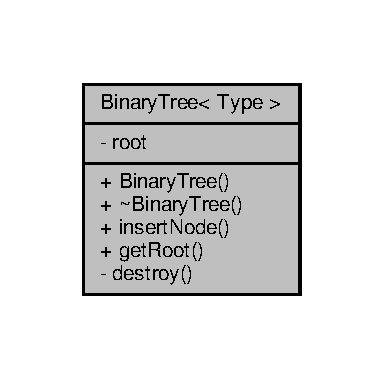
\includegraphics[width=184pt]{class_binary_tree__coll__graph}
\end{center}
\end{figure}
\subsection*{Public Member Functions}
\begin{DoxyCompactItemize}
\item 
\hyperlink{class_binary_tree_a9f5a2d791e391c6195ef290303973e15}{Binary\+Tree} ()
\item 
virtual \hyperlink{class_binary_tree_a2bad873a7fc094d66a3076a86d11c428}{$\sim$\+Binary\+Tree} ()
\item 
void \hyperlink{class_binary_tree_a69ae782d438253d40cbd194737feca17}{insert\+Node} (Type $\ast$data)
\item 
const \hyperlink{class_node}{Node}$<$ Type $>$ $\ast$ \hyperlink{class_binary_tree_a9ee0cf09781cf2ecc471aacc61848dde}{get\+Root} () const
\end{DoxyCompactItemize}
\subsection*{Private Member Functions}
\begin{DoxyCompactItemize}
\item 
void \hyperlink{class_binary_tree_a9b20827d019844170bb09465f885fef4}{destroy} (\hyperlink{class_node}{Node}$<$ Type $>$ $\ast$tmp)
\end{DoxyCompactItemize}
\subsection*{Private Attributes}
\begin{DoxyCompactItemize}
\item 
\hyperlink{class_node}{Node}$<$ Type $>$ $\ast$ \hyperlink{class_binary_tree_a8744322abfc99966f7d23d8560ed5702}{root}
\end{DoxyCompactItemize}


\subsection{Detailed Description}
\subsubsection*{template$<$class Type$>$\newline
class Binary\+Tree$<$ Type $>$}

Generic class \hyperlink{class_binary_tree}{Binary\+Tree} defines the binary tree 
\begin{DoxyTemplParams}{Template Parameters}
{\em Type} & \\
\hline
\end{DoxyTemplParams}


Definition at line 54 of file Binary\+Tree.\+h.



\subsection{Constructor \& Destructor Documentation}
\mbox{\Hypertarget{class_binary_tree_a9f5a2d791e391c6195ef290303973e15}\label{class_binary_tree_a9f5a2d791e391c6195ef290303973e15}} 
\index{Binary\+Tree@{Binary\+Tree}!Binary\+Tree@{Binary\+Tree}}
\index{Binary\+Tree@{Binary\+Tree}!Binary\+Tree@{Binary\+Tree}}
\subsubsection{\texorpdfstring{Binary\+Tree()}{BinaryTree()}}
{\footnotesize\ttfamily template$<$class Type$>$ \\
\hyperlink{class_binary_tree}{Binary\+Tree}$<$ Type $>$\+::\hyperlink{class_binary_tree}{Binary\+Tree} (\begin{DoxyParamCaption}{ }\end{DoxyParamCaption})\hspace{0.3cm}{\ttfamily [inline]}}

constructor function 

Definition at line 59 of file Binary\+Tree.\+h.


\begin{DoxyCode}
59                 \{
60         \hyperlink{class_binary_tree_a8744322abfc99966f7d23d8560ed5702}{root} = 0;
61     \}
\end{DoxyCode}
\mbox{\Hypertarget{class_binary_tree_a2bad873a7fc094d66a3076a86d11c428}\label{class_binary_tree_a2bad873a7fc094d66a3076a86d11c428}} 
\index{Binary\+Tree@{Binary\+Tree}!````~Binary\+Tree@{$\sim$\+Binary\+Tree}}
\index{````~Binary\+Tree@{$\sim$\+Binary\+Tree}!Binary\+Tree@{Binary\+Tree}}
\subsubsection{\texorpdfstring{$\sim$\+Binary\+Tree()}{~BinaryTree()}}
{\footnotesize\ttfamily template$<$class Type$>$ \\
virtual \hyperlink{class_binary_tree}{Binary\+Tree}$<$ Type $>$\+::$\sim$\hyperlink{class_binary_tree}{Binary\+Tree} (\begin{DoxyParamCaption}{ }\end{DoxyParamCaption})\hspace{0.3cm}{\ttfamily [inline]}, {\ttfamily [virtual]}}

destructor function deletes the nodes in the tree and destroys the tree 

Definition at line 66 of file Binary\+Tree.\+h.


\begin{DoxyCode}
66                          \{
67         \hyperlink{class_binary_tree_a9b20827d019844170bb09465f885fef4}{destroy}(\hyperlink{class_binary_tree_a8744322abfc99966f7d23d8560ed5702}{root});
68     \}
\end{DoxyCode}


\subsection{Member Function Documentation}
\mbox{\Hypertarget{class_binary_tree_a9b20827d019844170bb09465f885fef4}\label{class_binary_tree_a9b20827d019844170bb09465f885fef4}} 
\index{Binary\+Tree@{Binary\+Tree}!destroy@{destroy}}
\index{destroy@{destroy}!Binary\+Tree@{Binary\+Tree}}
\subsubsection{\texorpdfstring{destroy()}{destroy()}}
{\footnotesize\ttfamily template$<$class Type$>$ \\
void \hyperlink{class_binary_tree}{Binary\+Tree}$<$ Type $>$\+::destroy (\begin{DoxyParamCaption}\item[{\hyperlink{class_node}{Node}$<$ Type $>$ $\ast$}]{tmp }\end{DoxyParamCaption})\hspace{0.3cm}{\ttfamily [inline]}, {\ttfamily [private]}}

function to destroy the binary tree 
\begin{DoxyParams}{Parameters}
{\em tmp} & \\
\hline
\end{DoxyParams}


Definition at line 123 of file Binary\+Tree.\+h.


\begin{DoxyCode}
123                                   \{
124         \textcolor{keywordflow}{if} (tmp != NULL)    \{
125             \hyperlink{class_binary_tree_a9b20827d019844170bb09465f885fef4}{destroy}(tmp->\hyperlink{class_node_abb08a8b3137dd8fc8874348a439e01b4}{left});
126             tmp->\hyperlink{class_node_abb08a8b3137dd8fc8874348a439e01b4}{left} = NULL;
127             \hyperlink{class_binary_tree_a9b20827d019844170bb09465f885fef4}{destroy}(tmp->\hyperlink{class_node_a34452c0684d3cb1590406ad201b43e65}{right});
128             tmp->\hyperlink{class_node_a34452c0684d3cb1590406ad201b43e65}{right} = NULL;
129             \textcolor{keyword}{delete} tmp;
130         \}
131     \}
\end{DoxyCode}
\mbox{\Hypertarget{class_binary_tree_a9ee0cf09781cf2ecc471aacc61848dde}\label{class_binary_tree_a9ee0cf09781cf2ecc471aacc61848dde}} 
\index{Binary\+Tree@{Binary\+Tree}!get\+Root@{get\+Root}}
\index{get\+Root@{get\+Root}!Binary\+Tree@{Binary\+Tree}}
\subsubsection{\texorpdfstring{get\+Root()}{getRoot()}}
{\footnotesize\ttfamily template$<$class Type$>$ \\
const \hyperlink{class_node}{Node}$<$Type$>$$\ast$ \hyperlink{class_binary_tree}{Binary\+Tree}$<$ Type $>$\+::get\+Root (\begin{DoxyParamCaption}{ }\end{DoxyParamCaption}) const\hspace{0.3cm}{\ttfamily [inline]}}

function to return root of the binary tree \begin{DoxyReturn}{Returns}
root of the binary tree 
\end{DoxyReturn}


Definition at line 114 of file Binary\+Tree.\+h.


\begin{DoxyCode}
114                                       \{
115         \textcolor{keywordflow}{return} \hyperlink{class_binary_tree_a8744322abfc99966f7d23d8560ed5702}{root};
116     \}
\end{DoxyCode}
Here is the caller graph for this function\+:
\nopagebreak
\begin{figure}[H]
\begin{center}
\leavevmode
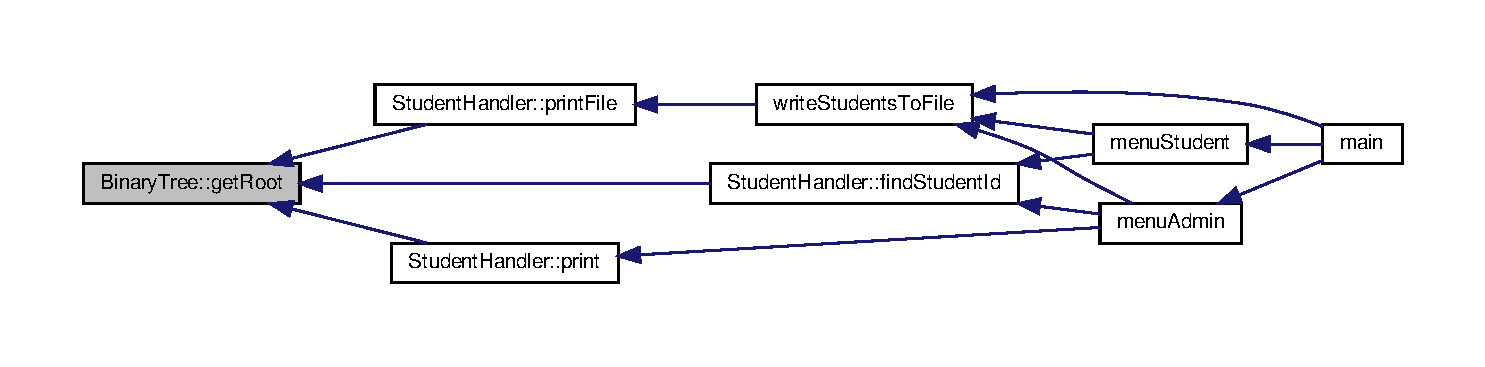
\includegraphics[width=350pt]{class_binary_tree_a9ee0cf09781cf2ecc471aacc61848dde_icgraph}
\end{center}
\end{figure}
\mbox{\Hypertarget{class_binary_tree_a69ae782d438253d40cbd194737feca17}\label{class_binary_tree_a69ae782d438253d40cbd194737feca17}} 
\index{Binary\+Tree@{Binary\+Tree}!insert\+Node@{insert\+Node}}
\index{insert\+Node@{insert\+Node}!Binary\+Tree@{Binary\+Tree}}
\subsubsection{\texorpdfstring{insert\+Node()}{insertNode()}}
{\footnotesize\ttfamily template$<$class Type$>$ \\
void \hyperlink{class_binary_tree}{Binary\+Tree}$<$ Type $>$\+::insert\+Node (\begin{DoxyParamCaption}\item[{Type $\ast$}]{data }\end{DoxyParamCaption})\hspace{0.3cm}{\ttfamily [inline]}}

function to insert a new node to the binary tree 
\begin{DoxyParams}{Parameters}
{\em data} & generic data of new node \\
\hline
\end{DoxyParams}


Definition at line 73 of file Binary\+Tree.\+h.


\begin{DoxyCode}
73                                  \{
74         \hyperlink{class_node}{Node <Type>} * temp = \textcolor{keyword}{new} \hyperlink{class_node}{Node<Type>}(data);
75 
76         \textcolor{keywordflow}{if}(\hyperlink{class_binary_tree_a8744322abfc99966f7d23d8560ed5702}{root} == 0)\{
77             \hyperlink{class_binary_tree_a8744322abfc99966f7d23d8560ed5702}{root} = temp;
78             \textcolor{keywordflow}{return};
79         \}
80         \textcolor{keywordflow}{else} \{
81             \hyperlink{classqueue_l_l}{queueLL<Node <Type>}> * queue = \textcolor{keyword}{new} 
      \hyperlink{classqueue_l_l}{queueLL<Node <Type>}>();
82             \textcolor{comment}{//Add root to the queue}
83             queue->\hyperlink{classqueue_l_l_adcbcc26433da2c9d17b6cf0802d1d7d2}{add}(\hyperlink{class_binary_tree_a8744322abfc99966f7d23d8560ed5702}{root});
84 
85             \textcolor{keywordflow}{while}(\textcolor{keyword}{true}) \{
86                 \hyperlink{class_node}{Node<Type>} * n = queue->\hyperlink{classqueue_l_l_a4204a9db973b69be5824ca2495130b40}{remove}();
87                 \textcolor{keywordflow}{if}(n!=0)\{
88                     \textcolor{keywordflow}{if}(n->\hyperlink{class_node_abb08a8b3137dd8fc8874348a439e01b4}{left} != 0 && n->\hyperlink{class_node_a34452c0684d3cb1590406ad201b43e65}{right} != 0) \{
89                         queue->\hyperlink{classqueue_l_l_adcbcc26433da2c9d17b6cf0802d1d7d2}{add}(n->\hyperlink{class_node_abb08a8b3137dd8fc8874348a439e01b4}{left});
90                         queue->\hyperlink{classqueue_l_l_adcbcc26433da2c9d17b6cf0802d1d7d2}{add}(n->\hyperlink{class_node_a34452c0684d3cb1590406ad201b43e65}{right});
91                     \}
92                     \textcolor{keywordflow}{else} \{
93                         \textcolor{keywordflow}{if}(n->\hyperlink{class_node_abb08a8b3137dd8fc8874348a439e01b4}{left} == 0) \{
94                          n->\hyperlink{class_node_abb08a8b3137dd8fc8874348a439e01b4}{left} = temp;
95                          queue->\hyperlink{classqueue_l_l_adcbcc26433da2c9d17b6cf0802d1d7d2}{add}(n->\hyperlink{class_node_abb08a8b3137dd8fc8874348a439e01b4}{left});
96                         \}
97                         \textcolor{comment}{//If node has left child but no right child, make newNode as right child}
98                         \textcolor{keywordflow}{else} \{
99                          n->\hyperlink{class_node_a34452c0684d3cb1590406ad201b43e65}{right} = temp;
100                          queue->\hyperlink{classqueue_l_l_adcbcc26433da2c9d17b6cf0802d1d7d2}{add}(n->\hyperlink{class_node_a34452c0684d3cb1590406ad201b43e65}{right});
101                         \}
102                         \textcolor{keywordflow}{break};
103                     \}
104                     \textcolor{comment}{//delete(n);}
105                 \}
106             \}
107             \textcolor{keyword}{delete}(queue);
108         \}
109     \}
\end{DoxyCode}
Here is the caller graph for this function\+:
\nopagebreak
\begin{figure}[H]
\begin{center}
\leavevmode
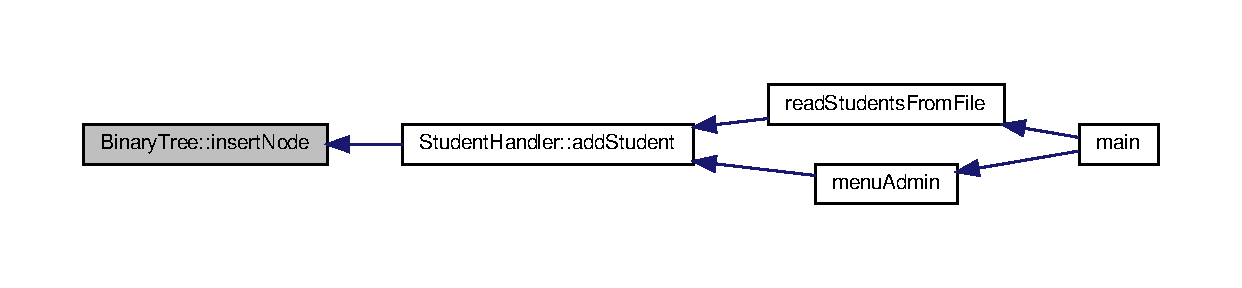
\includegraphics[width=350pt]{class_binary_tree_a69ae782d438253d40cbd194737feca17_icgraph}
\end{center}
\end{figure}


\subsection{Member Data Documentation}
\mbox{\Hypertarget{class_binary_tree_a8744322abfc99966f7d23d8560ed5702}\label{class_binary_tree_a8744322abfc99966f7d23d8560ed5702}} 
\index{Binary\+Tree@{Binary\+Tree}!root@{root}}
\index{root@{root}!Binary\+Tree@{Binary\+Tree}}
\subsubsection{\texorpdfstring{root}{root}}
{\footnotesize\ttfamily template$<$class Type$>$ \\
\hyperlink{class_node}{Node}$<$Type$>$$\ast$ \hyperlink{class_binary_tree}{Binary\+Tree}$<$ Type $>$\+::root\hspace{0.3cm}{\ttfamily [private]}}

root of the the binary tree 

Definition at line 136 of file Binary\+Tree.\+h.



The documentation for this class was generated from the following file\+:\begin{DoxyCompactItemize}
\item 
src/\hyperlink{_binary_tree_8h}{Binary\+Tree.\+h}\end{DoxyCompactItemize}

\hypertarget{classbook}{}\section{book Class Reference}
\label{classbook}\index{book@{book}}


{\ttfamily \#include $<$Book.\+h$>$}



Collaboration diagram for book\+:
\nopagebreak
\begin{figure}[H]
\begin{center}
\leavevmode
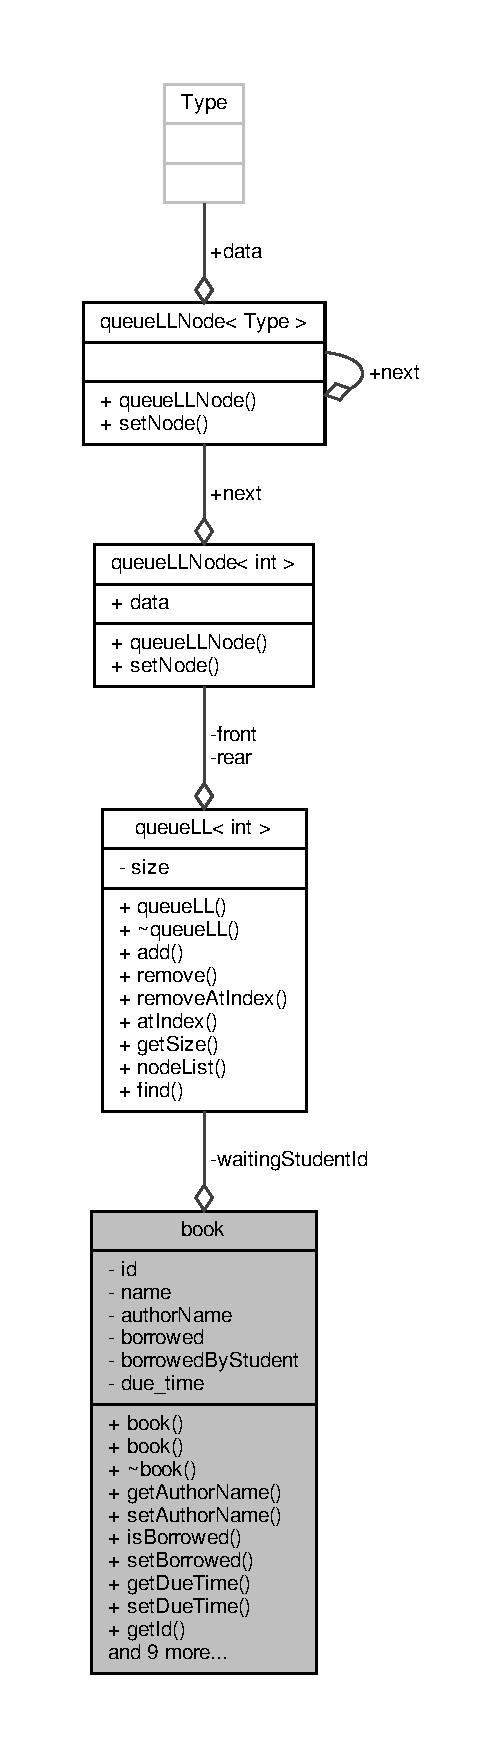
\includegraphics[height=550pt]{classbook__coll__graph}
\end{center}
\end{figure}
\subsection*{Public Member Functions}
\begin{DoxyCompactItemize}
\item 
\hyperlink{classbook_ad081661f16222b7195ff4342ba4fdf04}{book} ()
\item 
\hyperlink{classbook_af51e1b11131e522f13d5c4b52a3eed03}{book} (std\+::string \hyperlink{classbook_a5eabc1c1c5abff26997bec3d41f90d9e}{name}, std\+::string auth\+Name)
\item 
virtual \hyperlink{classbook_a807e512df9551f568ed2b7bae11f3884}{$\sim$book} ()
\item 
const std\+::string \& \hyperlink{classbook_a8cfa3bc064dafb1fde6bd997d0075df9}{get\+Author\+Name} () const
\item 
void \hyperlink{classbook_ab6da44e6c1680a8e802a14c2fcd20e78}{set\+Author\+Name} (const std\+::string \&\hyperlink{classbook_a21b2962c6227818732db27f12121b732}{author\+Name})
\item 
bool \hyperlink{classbook_aa76dd75565c10ec36c0f4649341b4fa1}{is\+Borrowed} () const
\item 
void \hyperlink{classbook_a7deed8c0520ef6f6b1dd5ebf9345cc72}{set\+Borrowed} (bool \hyperlink{classbook_ab745520ed537e69bde6f2e3d7a103276}{borrowed})
\item 
const tm \hyperlink{classbook_aa8eda0350d5882656cf53321d559c277}{get\+Due\+Time} () const
\item 
void \hyperlink{classbook_a61624bab2476a61fb2f27ebf7c8976e3}{set\+Due\+Time} ()
\item 
int \hyperlink{classbook_ab0c28db5fce5e04944c8ead875ce0e6a}{get\+Id} () const
\item 
const std\+::string \& \hyperlink{classbook_ae03ca5596d9b2a5992cc9da95d04e0cb}{get\+Name} () const
\item 
void \hyperlink{classbook_a40395f6b694a4c816bcf7a0ef279cf26}{set\+Name} (const std\+::string \&\hyperlink{classbook_a5eabc1c1c5abff26997bec3d41f90d9e}{name})
\item 
void \hyperlink{classbook_a458d26a8ddd01f69083a68eb68bf2181}{to\+String} (std\+::string \&out)
\item 
bool \hyperlink{classbook_a68bc47d79edd93594d50f720be2653f6}{borrow\+Book} (int $\ast$student\+Id)
\item 
int \hyperlink{classbook_af11d02d9964b788986dc8e26d1cdf373}{return\+Book} ()
\item 
int \hyperlink{classbook_a51aa01018a7c1569388aac015578e057}{get\+Borrowed\+By\+Student} () const
\item 
bool \hyperlink{classbook_acf51be6cb1a1e98d461144e134583c8f}{parse\+Line} (std\+::string \&line)
\item 
void \hyperlink{classbook_aea835c54459ec0a4d29d42f2f6f7858d}{create\+Line} (std\+::string \&line)
\item 
void \hyperlink{classbook_a73dd64c834bd70d659ee456f3ef94c05}{add\+B\+O\+O\+K\+\_\+\+C\+O\+U\+NT} ()
\end{DoxyCompactItemize}
\subsection*{Private Attributes}
\begin{DoxyCompactItemize}
\item 
int \hyperlink{classbook_ad8bf54b50c72af3827823c04d724d824}{id}
\item 
std\+::string \hyperlink{classbook_a5eabc1c1c5abff26997bec3d41f90d9e}{name}
\item 
std\+::string \hyperlink{classbook_a21b2962c6227818732db27f12121b732}{author\+Name}
\item 
bool \hyperlink{classbook_ab745520ed537e69bde6f2e3d7a103276}{borrowed}
\item 
int \hyperlink{classbook_afa5350900be6a34d8301a57d6db54df5}{borrowed\+By\+Student}
\item 
tm \hyperlink{classbook_abf72d9a32cdadee632df5a626dbe33b8}{due\+\_\+time}
\item 
\hyperlink{classqueue_l_l}{queue\+LL}$<$ int $>$ $\ast$ \hyperlink{classbook_a40ce04fcfbf99ffdbe7a4e1463588ee5}{waiting\+Student\+Id}
\end{DoxyCompactItemize}
\subsection*{Friends}
\begin{DoxyCompactItemize}
\item 
std\+::ostream \& \hyperlink{classbook_a9bd0243ea50c5b8c37ed0d5527f24177}{operator$<$$<$} (std\+::ostream \&out, const \hyperlink{classbook}{book} \&b)
\item 
bool \hyperlink{classbook_af7856e28b06865a9691d5c7a330633a4}{operator!=} (const \hyperlink{classbook}{book} \&b1, const \hyperlink{classbook}{book} \&b2)
\item 
bool \hyperlink{classbook_a3d386e1f8255c6b62d9858fb8ff41c86}{operator$<$} (\hyperlink{classbook}{book} \&b1, \hyperlink{classbook}{book} \&b2)
\end{DoxyCompactItemize}


\subsection{Detailed Description}
Class book shows all the functions and members of a book 

Definition at line 25 of file Book.\+h.



\subsection{Constructor \& Destructor Documentation}
\mbox{\Hypertarget{classbook_ad081661f16222b7195ff4342ba4fdf04}\label{classbook_ad081661f16222b7195ff4342ba4fdf04}} 
\index{book@{book}!book@{book}}
\index{book@{book}!book@{book}}
\subsubsection{\texorpdfstring{book()}{book()}\hspace{0.1cm}{\footnotesize\ttfamily [1/2]}}
{\footnotesize\ttfamily book\+::book (\begin{DoxyParamCaption}{ }\end{DoxyParamCaption})}

constructor function 

Definition at line 11 of file Book.\+cpp.


\begin{DoxyCode}
11            \{
12     \textcolor{keywordtype}{id} = -1;
13     \hyperlink{classbook_a5eabc1c1c5abff26997bec3d41f90d9e}{name} = \textcolor{stringliteral}{" "};
14     \hyperlink{classbook_a21b2962c6227818732db27f12121b732}{authorName} = \textcolor{stringliteral}{" "};
15     \hyperlink{classbook_ab745520ed537e69bde6f2e3d7a103276}{borrowed} = \textcolor{keyword}{false};
16     time\_t now = time( NULL);
17     \hyperlink{classbook_abf72d9a32cdadee632df5a626dbe33b8}{due\_time} = *localtime( &now);
18     \hyperlink{classbook_a40ce04fcfbf99ffdbe7a4e1463588ee5}{waitingStudentId} = \textcolor{keyword}{new} \hyperlink{classqueue_l_l}{queueLL<int>}();
19     \hyperlink{classbook_afa5350900be6a34d8301a57d6db54df5}{borrowedByStudent} = -1;
20 \}
\end{DoxyCode}
\mbox{\Hypertarget{classbook_af51e1b11131e522f13d5c4b52a3eed03}\label{classbook_af51e1b11131e522f13d5c4b52a3eed03}} 
\index{book@{book}!book@{book}}
\index{book@{book}!book@{book}}
\subsubsection{\texorpdfstring{book()}{book()}\hspace{0.1cm}{\footnotesize\ttfamily [2/2]}}
{\footnotesize\ttfamily book\+::book (\begin{DoxyParamCaption}\item[{std\+::string}]{name,  }\item[{std\+::string}]{auth\+Name }\end{DoxyParamCaption})}

constructor function 
\begin{DoxyParams}{Parameters}
{\em name} & book name \\
\hline
{\em auth\+Name} & author name \\
\hline
\end{DoxyParams}


Definition at line 22 of file Book.\+cpp.


\begin{DoxyCode}
22                                              \{
23     \textcolor{keywordtype}{id} = ++\hyperlink{_book_8h_a84e48ab264903213f7f7a264da4e867d}{BOOK\_COUNT};
24     this->\hyperlink{classbook_a5eabc1c1c5abff26997bec3d41f90d9e}{name} = \hyperlink{classbook_a5eabc1c1c5abff26997bec3d41f90d9e}{name};
25     this->\hyperlink{classbook_a21b2962c6227818732db27f12121b732}{authorName} = authName;
26     \hyperlink{classbook_ab745520ed537e69bde6f2e3d7a103276}{borrowed} = \textcolor{keyword}{false};
27     time\_t now = time( NULL);
28     \hyperlink{classbook_abf72d9a32cdadee632df5a626dbe33b8}{due\_time} = *localtime( &now);
29     \hyperlink{classbook_a40ce04fcfbf99ffdbe7a4e1463588ee5}{waitingStudentId} = \textcolor{keyword}{new} \hyperlink{classqueue_l_l}{queueLL<int>}();
30     \hyperlink{classbook_afa5350900be6a34d8301a57d6db54df5}{borrowedByStudent} = -1;
31 \}
\end{DoxyCode}
\mbox{\Hypertarget{classbook_a807e512df9551f568ed2b7bae11f3884}\label{classbook_a807e512df9551f568ed2b7bae11f3884}} 
\index{book@{book}!````~book@{$\sim$book}}
\index{````~book@{$\sim$book}!book@{book}}
\subsubsection{\texorpdfstring{$\sim$book()}{~book()}}
{\footnotesize\ttfamily book\+::$\sim$book (\begin{DoxyParamCaption}{ }\end{DoxyParamCaption})\hspace{0.3cm}{\ttfamily [virtual]}}

destructor function 

Definition at line 34 of file Book.\+cpp.


\begin{DoxyCode}
34             \{
35 
36 \}
\end{DoxyCode}


\subsection{Member Function Documentation}
\mbox{\Hypertarget{classbook_a73dd64c834bd70d659ee456f3ef94c05}\label{classbook_a73dd64c834bd70d659ee456f3ef94c05}} 
\index{book@{book}!add\+B\+O\+O\+K\+\_\+\+C\+O\+U\+NT@{add\+B\+O\+O\+K\+\_\+\+C\+O\+U\+NT}}
\index{add\+B\+O\+O\+K\+\_\+\+C\+O\+U\+NT@{add\+B\+O\+O\+K\+\_\+\+C\+O\+U\+NT}!book@{book}}
\subsubsection{\texorpdfstring{add\+B\+O\+O\+K\+\_\+\+C\+O\+U\+N\+T()}{addBOOK\_COUNT()}}
{\footnotesize\ttfamily void book\+::add\+B\+O\+O\+K\+\_\+\+C\+O\+U\+NT (\begin{DoxyParamCaption}{ }\end{DoxyParamCaption})}



Definition at line 333 of file Book.\+cpp.


\begin{DoxyCode}
333                         \{
334     ++\hyperlink{_book_8h_a84e48ab264903213f7f7a264da4e867d}{BOOK\_COUNT};
335 \}
\end{DoxyCode}
Here is the caller graph for this function\+:
\nopagebreak
\begin{figure}[H]
\begin{center}
\leavevmode
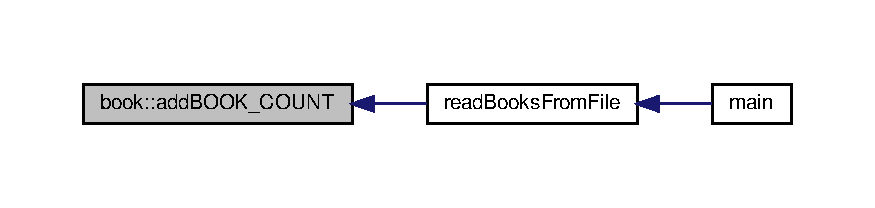
\includegraphics[width=350pt]{classbook_a73dd64c834bd70d659ee456f3ef94c05_icgraph}
\end{center}
\end{figure}
\mbox{\Hypertarget{classbook_a68bc47d79edd93594d50f720be2653f6}\label{classbook_a68bc47d79edd93594d50f720be2653f6}} 
\index{book@{book}!borrow\+Book@{borrow\+Book}}
\index{borrow\+Book@{borrow\+Book}!book@{book}}
\subsubsection{\texorpdfstring{borrow\+Book()}{borrowBook()}}
{\footnotesize\ttfamily bool book\+::borrow\+Book (\begin{DoxyParamCaption}\item[{int $\ast$}]{student\+Id }\end{DoxyParamCaption})}

function to borrow book 
\begin{DoxyParams}{Parameters}
{\em student\+Id} & id of student \\
\hline
\end{DoxyParams}
\begin{DoxyReturn}{Returns}
true, if book is borrowed to student\+Id. false, if book is not borrowed and student\+If is added to waiting\+Student\+Id 
\end{DoxyReturn}


Definition at line 104 of file Book.\+cpp.


\begin{DoxyCode}
104                                      \{
105     \textcolor{keywordtype}{bool} returnValue = \textcolor{keyword}{false};
106     \textcolor{keywordflow}{if}( \hyperlink{classbook_ab745520ed537e69bde6f2e3d7a103276}{borrowed} == \textcolor{keyword}{true} && \hyperlink{classbook_afa5350900be6a34d8301a57d6db54df5}{borrowedByStudent} == *studentId)\{
107         std::cout<<\textcolor{stringliteral}{"STUDENT "}<<*studentId<<\textcolor{stringliteral}{" ALREADY BORROWED THE BOOK\(\backslash\)n"};
108     \}
109     \textcolor{keywordflow}{else} \textcolor{keywordflow}{if}( \hyperlink{classbook_ab745520ed537e69bde6f2e3d7a103276}{borrowed} == \textcolor{keyword}{true} && \hyperlink{classbook_a40ce04fcfbf99ffdbe7a4e1463588ee5}{waitingStudentId}->\hyperlink{classqueue_l_l_af46d9d07b7528da834c2c37d752c29f5}{find}(*studentId) > -1  )\{
110             std::cout<<\textcolor{stringliteral}{"STUDENT "}<<*studentId<<\textcolor{stringliteral}{" ALREADY IS IN WAITING LIST\(\backslash\)n"};
111         \}
112     \textcolor{keywordflow}{else} \textcolor{keywordflow}{if}(\hyperlink{classbook_ab745520ed537e69bde6f2e3d7a103276}{borrowed} == \textcolor{keyword}{true})\{
113         \hyperlink{classbook_a40ce04fcfbf99ffdbe7a4e1463588ee5}{waitingStudentId}->\hyperlink{classqueue_l_l_adcbcc26433da2c9d17b6cf0802d1d7d2}{add}(studentId);
114         std::cout<<\textcolor{stringliteral}{"STUDENT "}<<*studentId<<\textcolor{stringliteral}{" ADDED TO WAITING LIST\(\backslash\)n"};
115     \}
116     \textcolor{keywordflow}{else}\{
117         \hyperlink{classbook_ab745520ed537e69bde6f2e3d7a103276}{borrowed} = \textcolor{keyword}{true};
118         \hyperlink{classbook_afa5350900be6a34d8301a57d6db54df5}{borrowedByStudent} = *studentId;
119         \hyperlink{classbook_a61624bab2476a61fb2f27ebf7c8976e3}{setDueTime}();
120         returnValue = \textcolor{keyword}{true};
121     \}
122     \textcolor{keywordflow}{return}  returnValue;
123 \}
\end{DoxyCode}
Here is the call graph for this function\+:
\nopagebreak
\begin{figure}[H]
\begin{center}
\leavevmode
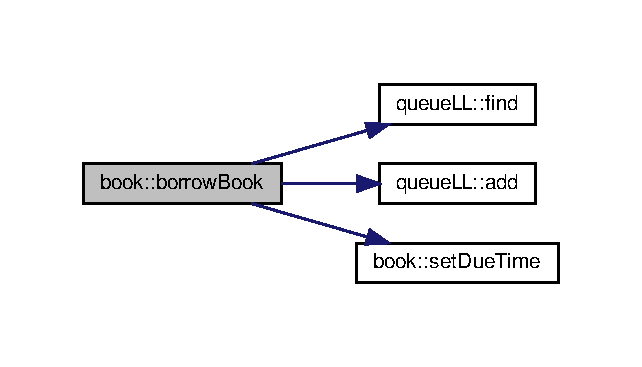
\includegraphics[width=308pt]{classbook_a68bc47d79edd93594d50f720be2653f6_cgraph}
\end{center}
\end{figure}
Here is the caller graph for this function\+:
\nopagebreak
\begin{figure}[H]
\begin{center}
\leavevmode
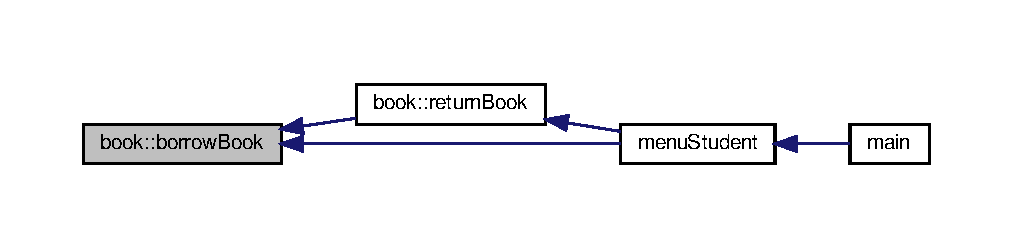
\includegraphics[width=350pt]{classbook_a68bc47d79edd93594d50f720be2653f6_icgraph}
\end{center}
\end{figure}
\mbox{\Hypertarget{classbook_aea835c54459ec0a4d29d42f2f6f7858d}\label{classbook_aea835c54459ec0a4d29d42f2f6f7858d}} 
\index{book@{book}!create\+Line@{create\+Line}}
\index{create\+Line@{create\+Line}!book@{book}}
\subsubsection{\texorpdfstring{create\+Line()}{createLine()}}
{\footnotesize\ttfamily void book\+::create\+Line (\begin{DoxyParamCaption}\item[{std\+::string \&}]{line }\end{DoxyParamCaption})}

function to create line for file 
\begin{DoxyParams}{Parameters}
{\em line} & line that is supposed to write to file \\
\hline
\end{DoxyParams}


Definition at line 312 of file Book.\+cpp.


\begin{DoxyCode}
312                                      \{
313     \textcolor{keywordflow}{if}(\hyperlink{classbook_ab745520ed537e69bde6f2e3d7a103276}{borrowed} == \textcolor{keyword}{true})\{
314         line = std::to\_string(\textcolor{keywordtype}{id}) + \textcolor{stringliteral}{","} + \hyperlink{classbook_a5eabc1c1c5abff26997bec3d41f90d9e}{name} + \textcolor{stringliteral}{","} + \hyperlink{classbook_a21b2962c6227818732db27f12121b732}{authorName} + \textcolor{stringliteral}{","} +
315                 std::to\_string(\hyperlink{classbook_afa5350900be6a34d8301a57d6db54df5}{borrowedByStudent}) + \textcolor{stringliteral}{","} +
316                 std::to\_string(\hyperlink{classbook_abf72d9a32cdadee632df5a626dbe33b8}{due\_time}.tm\_year) + \textcolor{stringliteral}{"/"} + std::to\_string(
      \hyperlink{classbook_abf72d9a32cdadee632df5a626dbe33b8}{due\_time}.tm\_mon) + \textcolor{stringliteral}{"/"} +
317                 std::to\_string(\hyperlink{classbook_abf72d9a32cdadee632df5a626dbe33b8}{due\_time}.tm\_mday) + \textcolor{stringliteral}{"-"} +
318                 std::to\_string(\hyperlink{classbook_abf72d9a32cdadee632df5a626dbe33b8}{due\_time}.tm\_hour) + \textcolor{stringliteral}{":"} + std::to\_string(
      \hyperlink{classbook_abf72d9a32cdadee632df5a626dbe33b8}{due\_time}.tm\_min) + \textcolor{stringliteral}{":"} +
319                 std::to\_string(\hyperlink{classbook_abf72d9a32cdadee632df5a626dbe33b8}{due\_time}.tm\_sec) ;
320         \textcolor{keywordflow}{if}(\hyperlink{classbook_a40ce04fcfbf99ffdbe7a4e1463588ee5}{waitingStudentId}->\hyperlink{classqueue_l_l_a8969feebcb563f0b489bc112422b9563}{getSize}()>0)
321             line.append( \textcolor{stringliteral}{","});
322         \textcolor{keywordflow}{for}( \textcolor{keywordtype}{int} i=0; i < \hyperlink{classbook_a40ce04fcfbf99ffdbe7a4e1463588ee5}{waitingStudentId}->\hyperlink{classqueue_l_l_a8969feebcb563f0b489bc112422b9563}{getSize}(); i++)\{
323             line.append(std::to\_string(*\hyperlink{classbook_a40ce04fcfbf99ffdbe7a4e1463588ee5}{waitingStudentId}->
      \hyperlink{classqueue_l_l_a6c8873be0f08b3b2e83a24469fbfaa5d}{atIndex}(i)->\hyperlink{classqueue_l_l_node_a20b1170d8c5852b7dc01e56fda4e4206}{data}));
324             line.append(\textcolor{stringliteral}{","});
325         \}
326     \}
327     \textcolor{keywordflow}{else}\{
328 \textcolor{comment}{//      line = std::to\_string(id) + "," + name + "," + authorName + "," ;}
329         line = std::to\_string(\textcolor{keywordtype}{id}) + \textcolor{stringliteral}{","} + \hyperlink{classbook_a5eabc1c1c5abff26997bec3d41f90d9e}{name} + \textcolor{stringliteral}{","} + \hyperlink{classbook_a21b2962c6227818732db27f12121b732}{authorName}  ;
330     \}
331 \}
\end{DoxyCode}
Here is the call graph for this function\+:
\nopagebreak
\begin{figure}[H]
\begin{center}
\leavevmode
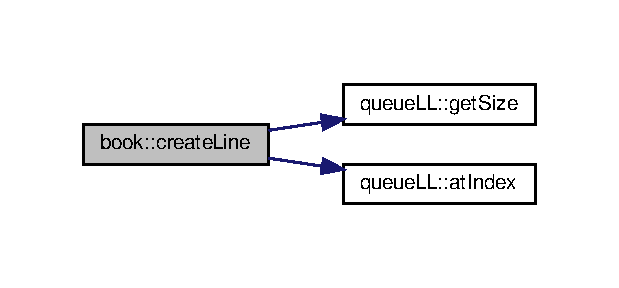
\includegraphics[width=297pt]{classbook_aea835c54459ec0a4d29d42f2f6f7858d_cgraph}
\end{center}
\end{figure}
Here is the caller graph for this function\+:
\nopagebreak
\begin{figure}[H]
\begin{center}
\leavevmode
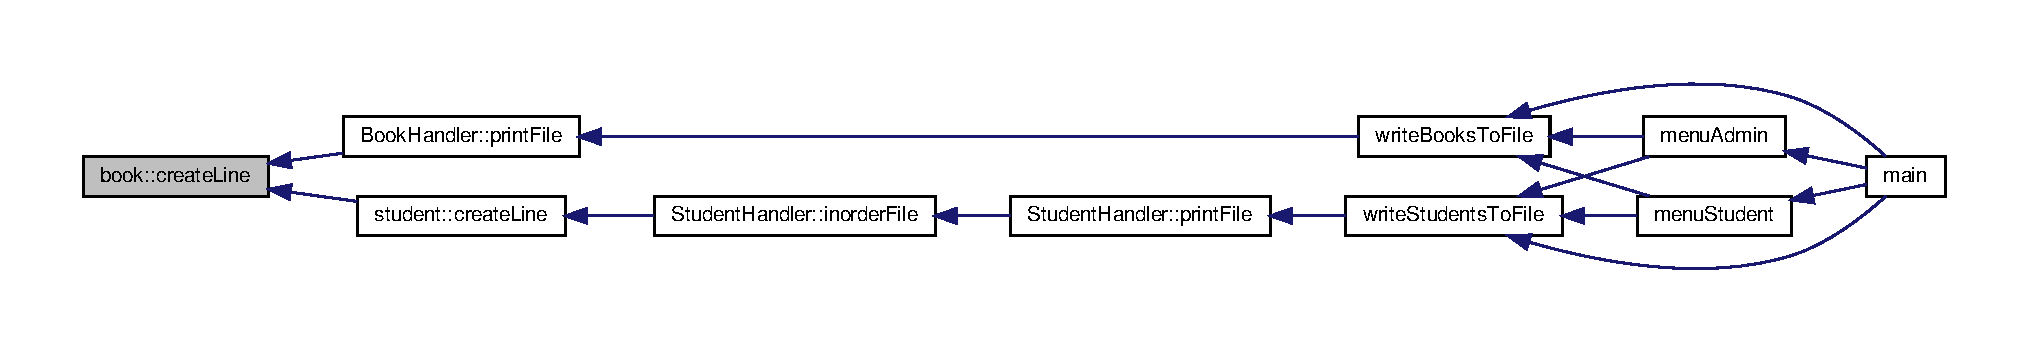
\includegraphics[width=350pt]{classbook_aea835c54459ec0a4d29d42f2f6f7858d_icgraph}
\end{center}
\end{figure}
\mbox{\Hypertarget{classbook_a8cfa3bc064dafb1fde6bd997d0075df9}\label{classbook_a8cfa3bc064dafb1fde6bd997d0075df9}} 
\index{book@{book}!get\+Author\+Name@{get\+Author\+Name}}
\index{get\+Author\+Name@{get\+Author\+Name}!book@{book}}
\subsubsection{\texorpdfstring{get\+Author\+Name()}{getAuthorName()}}
{\footnotesize\ttfamily const std\+::string \& book\+::get\+Author\+Name (\begin{DoxyParamCaption}{ }\end{DoxyParamCaption}) const}

function returns the name of the author \begin{DoxyReturn}{Returns}
the name of the author 
\end{DoxyReturn}


Definition at line 38 of file Book.\+cpp.


\begin{DoxyCode}
38                                            \{
39     \textcolor{keywordflow}{return} \hyperlink{classbook_a21b2962c6227818732db27f12121b732}{authorName};
40 \}
\end{DoxyCode}
\mbox{\Hypertarget{classbook_a51aa01018a7c1569388aac015578e057}\label{classbook_a51aa01018a7c1569388aac015578e057}} 
\index{book@{book}!get\+Borrowed\+By\+Student@{get\+Borrowed\+By\+Student}}
\index{get\+Borrowed\+By\+Student@{get\+Borrowed\+By\+Student}!book@{book}}
\subsubsection{\texorpdfstring{get\+Borrowed\+By\+Student()}{getBorrowedByStudent()}}
{\footnotesize\ttfamily int book\+::get\+Borrowed\+By\+Student (\begin{DoxyParamCaption}{ }\end{DoxyParamCaption}) const}

function returns id of the student that borrowed the book student \begin{DoxyReturn}{Returns}
id of the student 
\end{DoxyReturn}


Definition at line 176 of file Book.\+cpp.


\begin{DoxyCode}
176                                      \{
177     \textcolor{keywordflow}{return} \hyperlink{classbook_afa5350900be6a34d8301a57d6db54df5}{borrowedByStudent};
178 \}
\end{DoxyCode}
\mbox{\Hypertarget{classbook_aa8eda0350d5882656cf53321d559c277}\label{classbook_aa8eda0350d5882656cf53321d559c277}} 
\index{book@{book}!get\+Due\+Time@{get\+Due\+Time}}
\index{get\+Due\+Time@{get\+Due\+Time}!book@{book}}
\subsubsection{\texorpdfstring{get\+Due\+Time()}{getDueTime()}}
{\footnotesize\ttfamily const tm book\+::get\+Due\+Time (\begin{DoxyParamCaption}{ }\end{DoxyParamCaption}) const}

function returns the due time \begin{DoxyReturn}{Returns}
the due time 
\end{DoxyReturn}


Definition at line 55 of file Book.\+cpp.


\begin{DoxyCode}
55                                 \{
56     \textcolor{keywordflow}{return} \hyperlink{classbook_abf72d9a32cdadee632df5a626dbe33b8}{due\_time};
57 \}
\end{DoxyCode}
\mbox{\Hypertarget{classbook_ab0c28db5fce5e04944c8ead875ce0e6a}\label{classbook_ab0c28db5fce5e04944c8ead875ce0e6a}} 
\index{book@{book}!get\+Id@{get\+Id}}
\index{get\+Id@{get\+Id}!book@{book}}
\subsubsection{\texorpdfstring{get\+Id()}{getId()}}
{\footnotesize\ttfamily int book\+::get\+Id (\begin{DoxyParamCaption}{ }\end{DoxyParamCaption}) const}

function returns the book id \begin{DoxyReturn}{Returns}
the book id 
\end{DoxyReturn}


Definition at line 68 of file Book.\+cpp.


\begin{DoxyCode}
68                       \{
69     \textcolor{keywordflow}{return} \hyperlink{classbook_ad8bf54b50c72af3827823c04d724d824}{id};
70 \}
\end{DoxyCode}
\mbox{\Hypertarget{classbook_ae03ca5596d9b2a5992cc9da95d04e0cb}\label{classbook_ae03ca5596d9b2a5992cc9da95d04e0cb}} 
\index{book@{book}!get\+Name@{get\+Name}}
\index{get\+Name@{get\+Name}!book@{book}}
\subsubsection{\texorpdfstring{get\+Name()}{getName()}}
{\footnotesize\ttfamily const std\+::string \& book\+::get\+Name (\begin{DoxyParamCaption}{ }\end{DoxyParamCaption}) const}

function returns the book name \begin{DoxyReturn}{Returns}
the book name 
\end{DoxyReturn}


Definition at line 72 of file Book.\+cpp.


\begin{DoxyCode}
72                                      \{
73     \textcolor{keywordflow}{return} \hyperlink{classbook_a5eabc1c1c5abff26997bec3d41f90d9e}{name};
74 \}
\end{DoxyCode}
\mbox{\Hypertarget{classbook_aa76dd75565c10ec36c0f4649341b4fa1}\label{classbook_aa76dd75565c10ec36c0f4649341b4fa1}} 
\index{book@{book}!is\+Borrowed@{is\+Borrowed}}
\index{is\+Borrowed@{is\+Borrowed}!book@{book}}
\subsubsection{\texorpdfstring{is\+Borrowed()}{isBorrowed()}}
{\footnotesize\ttfamily bool book\+::is\+Borrowed (\begin{DoxyParamCaption}{ }\end{DoxyParamCaption}) const}

function shows if the books is borrowed or not \begin{DoxyReturn}{Returns}
true, if the book is borrowed. false, if the book is not borrowed 
\end{DoxyReturn}


Definition at line 47 of file Book.\+cpp.


\begin{DoxyCode}
47                             \{
48     \textcolor{keywordflow}{return} \hyperlink{classbook_ab745520ed537e69bde6f2e3d7a103276}{borrowed};
49 \}
\end{DoxyCode}
\mbox{\Hypertarget{classbook_acf51be6cb1a1e98d461144e134583c8f}\label{classbook_acf51be6cb1a1e98d461144e134583c8f}} 
\index{book@{book}!parse\+Line@{parse\+Line}}
\index{parse\+Line@{parse\+Line}!book@{book}}
\subsubsection{\texorpdfstring{parse\+Line()}{parseLine()}}
{\footnotesize\ttfamily bool book\+::parse\+Line (\begin{DoxyParamCaption}\item[{std\+::string \&}]{line }\end{DoxyParamCaption})}

function to parse line from file 
\begin{DoxyParams}{Parameters}
{\em line} & line that is read from file \\
\hline
\end{DoxyParams}
\begin{DoxyReturn}{Returns}
true, if parse is successful 
\end{DoxyReturn}


Definition at line 180 of file Book.\+cpp.


\begin{DoxyCode}
180                                     \{
181 
182     \textcolor{keywordtype}{bool} result = \textcolor{keyword}{false};
183 
184     std::stringstream check1(line);
185     std::string intermediate;
186 
187     \textcolor{keywordflow}{if}(std::getline(check1, intermediate, \textcolor{charliteral}{','}))\{\textcolor{comment}{//id}
188         \textcolor{keywordtype}{id} =  std::stoi(intermediate);
189             \textcolor{keywordflow}{if}(std::getline(check1, intermediate, \textcolor{charliteral}{','}))\{\textcolor{comment}{//name}
190                 \hyperlink{classbook_a5eabc1c1c5abff26997bec3d41f90d9e}{name} = intermediate;
191                 \textcolor{keywordflow}{if}(std::getline(check1, intermediate, \textcolor{charliteral}{','}))\{\textcolor{comment}{//author name}
192                     \hyperlink{classbook_a21b2962c6227818732db27f12121b732}{authorName} = intermediate;
193                     result = \textcolor{keyword}{true};
194                     \textcolor{keywordflow}{if}(std::getline(check1, intermediate, \textcolor{charliteral}{','}))\{\textcolor{comment}{//borrowed by student}
195                         \hyperlink{classbook_ab745520ed537e69bde6f2e3d7a103276}{borrowed} = \textcolor{keyword}{true};
196                         \hyperlink{classbook_afa5350900be6a34d8301a57d6db54df5}{borrowedByStudent} =  std::stoi(intermediate);
197                         \textcolor{keywordflow}{if}(std::getline(check1, intermediate, \textcolor{charliteral}{'/'}))\{\textcolor{comment}{//year}
198                             \hyperlink{classbook_abf72d9a32cdadee632df5a626dbe33b8}{due\_time}.tm\_year =  std::stoi(intermediate);
199                             \textcolor{keywordflow}{if}(std::getline(check1, intermediate, \textcolor{charliteral}{'/'}))\{\textcolor{comment}{//month}
200                                 \hyperlink{classbook_abf72d9a32cdadee632df5a626dbe33b8}{due\_time}.tm\_mon =  std::stoi(intermediate);
201                                 \textcolor{keywordflow}{if}(std::getline(check1, intermediate, \textcolor{charliteral}{'-'}))\{\textcolor{comment}{//day}
202                                     \hyperlink{classbook_abf72d9a32cdadee632df5a626dbe33b8}{due\_time}.tm\_mday =  std::stoi(intermediate);
203                                     \textcolor{keywordflow}{if}(std::getline(check1, intermediate, \textcolor{charliteral}{':'}))\{\textcolor{comment}{//hour}
204                                         \hyperlink{classbook_abf72d9a32cdadee632df5a626dbe33b8}{due\_time}.tm\_hour =  std::stoi(intermediate);
205                                         \textcolor{keywordflow}{if}(std::getline(check1, intermediate, \textcolor{charliteral}{':'}))\{\textcolor{comment}{//min}
206                                             \hyperlink{classbook_abf72d9a32cdadee632df5a626dbe33b8}{due\_time}.tm\_mon =  std::stoi(intermediate);
207                                             \textcolor{keywordflow}{if}(std::getline(check1, intermediate, \textcolor{charliteral}{','}))\{\textcolor{comment}{//sec}
208                                                 \hyperlink{classbook_abf72d9a32cdadee632df5a626dbe33b8}{due\_time}.tm\_sec=  std::stoi(intermediate);
209                                                 \textcolor{keywordflow}{if}(std::getline(check1, intermediate, \textcolor{charliteral}{','}))\{\textcolor{comment}{//waiting
       student id}
210                                                     \textcolor{keywordtype}{int} * n = \textcolor{keyword}{new} int( std::stoi(intermediate) );
211                                                     \hyperlink{classbook_a40ce04fcfbf99ffdbe7a4e1463588ee5}{waitingStudentId}->
      \hyperlink{classqueue_l_l_adcbcc26433da2c9d17b6cf0802d1d7d2}{add}(n);
212 
213                                                     std::vector <int> tokens;
214                                                     \textcolor{keywordflow}{while}(getline(check1, intermediate, \textcolor{charliteral}{','}))\{
215                                                         tokens.push\_back(std::stoi(intermediate));
216                                                     \}
217                                                     \textcolor{keywordflow}{for}(\textcolor{keywordtype}{int} i = 0; i < tokens.size(); i++)\{
218                                                         \textcolor{keywordtype}{int} *temp = \textcolor{keyword}{new} int( tokens[i] );
219                                                         \hyperlink{classbook_a40ce04fcfbf99ffdbe7a4e1463588ee5}{waitingStudentId}->
      \hyperlink{classqueue_l_l_adcbcc26433da2c9d17b6cf0802d1d7d2}{add}(temp);
220                                                     \}
221                                                 \}
222                                             \}
223                                         \}
224                                     \}
225                                 \}
226                             \}
227                         \}
228                     \}
229                 \}
230 
231             \}
232     \}
233 \textcolor{comment}{/*  char  cLine[line.size()+1];}
234 \textcolor{comment}{    bool result = false;}
235 \textcolor{comment}{    strcpy(cLine, line.c\_str());}
236 \textcolor{comment}{    char * tokenPtr = NULL;}
237 \textcolor{comment}{    //get id}
238 \textcolor{comment}{    tokenPtr = strtok (cLine,",");}
239 \textcolor{comment}{    if (tokenPtr != NULL)\{}
240 \textcolor{comment}{        id = atoi(tokenPtr);}
241 \textcolor{comment}{        //get name}
242 \textcolor{comment}{        tokenPtr = strtok (NULL, ",");}
243 \textcolor{comment}{        if (tokenPtr != NULL)\{}
244 \textcolor{comment}{            name = tokenPtr;}
245 \textcolor{comment}{            //get author}
246 \textcolor{comment}{            tokenPtr = strtok (NULL, ",");}
247 \textcolor{comment}{            if (tokenPtr != NULL)\{}
248 \textcolor{comment}{                authorName = tokenPtr;}
249 \textcolor{comment}{                result = true;}
250 \textcolor{comment}{                //borrowedByStudent}
251 \textcolor{comment}{                tokenPtr = strtok (NULL, ",");}
252 \textcolor{comment}{                    if (tokenPtr != NULL)\{}
253 \textcolor{comment}{                        borrowed = true;}
254 \textcolor{comment}{                        borrowedByStudent = atoi(tokenPtr);}
255 \textcolor{comment}{                        //year}
256 \textcolor{comment}{                        tokenPtr = strtok (NULL, ",");}
257 \textcolor{comment}{                        if (tokenPtr != NULL)\{}
258 \textcolor{comment}{                            due\_time.tm\_year = atoi(tokenPtr);}
259 \textcolor{comment}{                            //month}
260 \textcolor{comment}{                            tokenPtr = strtok (NULL, "/");}
261 \textcolor{comment}{                            if (tokenPtr != NULL)\{}
262 \textcolor{comment}{                                due\_time.tm\_mon = atoi(tokenPtr);}
263 \textcolor{comment}{                                //day}
264 \textcolor{comment}{                                tokenPtr = strtok (NULL, "/");}
265 \textcolor{comment}{                                if (tokenPtr != NULL)\{}
266 \textcolor{comment}{                                    due\_time.tm\_mday = atoi(tokenPtr);}
267 \textcolor{comment}{                                    //hour}
268 \textcolor{comment}{                                    tokenPtr = strtok (NULL, "-");}
269 \textcolor{comment}{                                    if (tokenPtr != NULL)\{}
270 \textcolor{comment}{                                        due\_time.tm\_hour = atoi(tokenPtr);}
271 \textcolor{comment}{                                        //min}
272 \textcolor{comment}{                                        tokenPtr = strtok (NULL, ":");}
273 \textcolor{comment}{                                        if (tokenPtr != NULL)\{}
274 \textcolor{comment}{                                            due\_time.tm\_min = atoi(tokenPtr);}
275 \textcolor{comment}{                                            //sec}
276 \textcolor{comment}{                                            tokenPtr = strtok (NULL, ":");}
277 \textcolor{comment}{                                            if (tokenPtr != NULL)\{}
278 \textcolor{comment}{                                                due\_time.tm\_sec = atoi(tokenPtr);}
279 \textcolor{comment}{                                                //waiting student id}
280 \textcolor{comment}{                                                tokenPtr = strtok (NULL, ",");}
281 \textcolor{comment}{                                                if (tokenPtr != NULL)\{}
282 \textcolor{comment}{                                                    int i = atoi(tokenPtr);}
283 \textcolor{comment}{                                                    waitingStudentId->add(&i);}
284 \textcolor{comment}{                                                    tokenPtr = strtok (NULL, " ");}
285 \textcolor{comment}{                                                    while (tokenPtr != NULL)\{}
286 \textcolor{comment}{                                                        int i = atoi(tokenPtr);}
287 \textcolor{comment}{                                                        waitingStudentId->add(&i);}
288 \textcolor{comment}{                                                        tokenPtr = strtok (NULL, " ");}
289 \textcolor{comment}{                                                    \}}
290 \textcolor{comment}{}
291 \textcolor{comment}{                                                \}//waiting student id}
292 \textcolor{comment}{                                            \}//sec}
293 \textcolor{comment}{                                        \}//min}
294 \textcolor{comment}{                                    \}//hour}
295 \textcolor{comment}{                                \}//day}
296 \textcolor{comment}{                            \}//month}
297 \textcolor{comment}{                        \}//year}
298 \textcolor{comment}{                    \}//borrowedByStudent}
299 \textcolor{comment}{                    else\{}
300 \textcolor{comment}{                        borrowed = false;}
301 \textcolor{comment}{                        time\_t now = time( NULL);}
302 \textcolor{comment}{                        due\_time = *localtime( &now);}
303 \textcolor{comment}{                        borrowedByStudent = -1;}
304 \textcolor{comment}{                    \}}
305 \textcolor{comment}{            \}//author}
306 \textcolor{comment}{        \}//name}
307 \textcolor{comment}{    \}//id}
308 \textcolor{comment}{    */}
309     \textcolor{keywordflow}{return} result;
310 \}
\end{DoxyCode}
Here is the call graph for this function\+:
\nopagebreak
\begin{figure}[H]
\begin{center}
\leavevmode
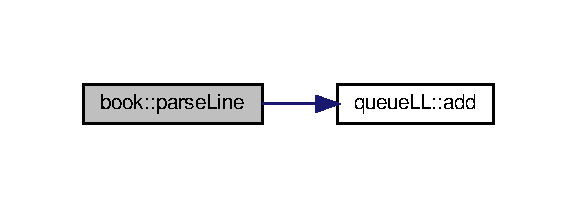
\includegraphics[width=277pt]{classbook_acf51be6cb1a1e98d461144e134583c8f_cgraph}
\end{center}
\end{figure}
Here is the caller graph for this function\+:
\nopagebreak
\begin{figure}[H]
\begin{center}
\leavevmode
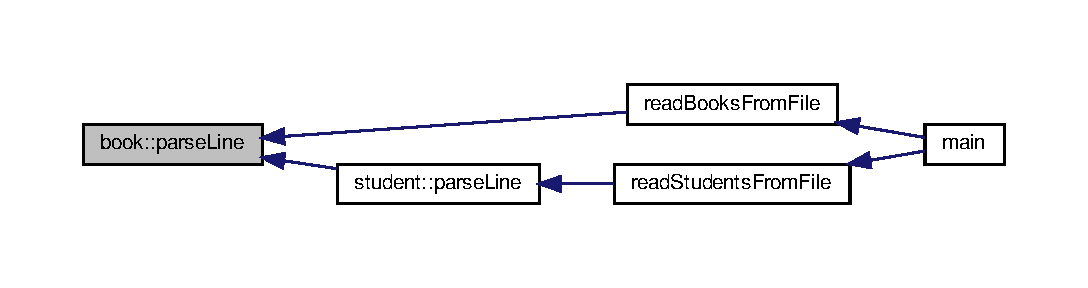
\includegraphics[width=350pt]{classbook_acf51be6cb1a1e98d461144e134583c8f_icgraph}
\end{center}
\end{figure}
\mbox{\Hypertarget{classbook_af11d02d9964b788986dc8e26d1cdf373}\label{classbook_af11d02d9964b788986dc8e26d1cdf373}} 
\index{book@{book}!return\+Book@{return\+Book}}
\index{return\+Book@{return\+Book}!book@{book}}
\subsubsection{\texorpdfstring{return\+Book()}{returnBook()}}
{\footnotesize\ttfamily int book\+::return\+Book (\begin{DoxyParamCaption}{ }\end{DoxyParamCaption})}

function to return book \begin{DoxyReturn}{Returns}
0 if book is returned. -\/1 if book can not be returned studentid if book is returned and borrowed by first student in waiting list 
\end{DoxyReturn}


Definition at line 80 of file Book.\+cpp.


\begin{DoxyCode}
80                      \{
81     \textcolor{keywordtype}{int} returnValue = -1;
82 
83     \textcolor{keywordflow}{if}(\hyperlink{classbook_ab745520ed537e69bde6f2e3d7a103276}{borrowed} == \textcolor{keyword}{true})\{
84         \hyperlink{classbook_afa5350900be6a34d8301a57d6db54df5}{borrowedByStudent} = -1;
85         \hyperlink{classbook_ab745520ed537e69bde6f2e3d7a103276}{borrowed} = \textcolor{keyword}{false};
86         \textcolor{keywordflow}{if}((\hyperlink{classbook_a40ce04fcfbf99ffdbe7a4e1463588ee5}{waitingStudentId}->\hyperlink{classqueue_l_l_a8969feebcb563f0b489bc112422b9563}{getSize}()) >0)\{
87             \textcolor{keywordtype}{int} * studentId = \hyperlink{classbook_a40ce04fcfbf99ffdbe7a4e1463588ee5}{waitingStudentId}->\hyperlink{classqueue_l_l_a4204a9db973b69be5824ca2495130b40}{remove}();
88             std::cout<<\textcolor{stringliteral}{"BOOK IS RETUNED AND IS BORROWED BY FIRST STUDENT "}
89                     <<*studentId<<\textcolor{stringliteral}{" IN WAITING LIST\(\backslash\)n"};
90             \hyperlink{classbook_a68bc47d79edd93594d50f720be2653f6}{borrowBook}(studentId);
91             returnValue = *studentId;
92         \}
93         \textcolor{keywordflow}{else}\{
94             std::cout<<\textcolor{stringliteral}{"BOOK IS RETUNED\(\backslash\)n"};
95             returnValue = 0;
96         \}
97     \}
98     \textcolor{keywordflow}{else}\{
99         std::cout<<\textcolor{stringliteral}{"BOOK IS NOT BORROWED AND CAN NOT BE RETURNED\(\backslash\)n"};
100         returnValue = -1;
101     \}
102     \textcolor{keywordflow}{return}  returnValue;
103 \}
\end{DoxyCode}
Here is the call graph for this function\+:
\nopagebreak
\begin{figure}[H]
\begin{center}
\leavevmode
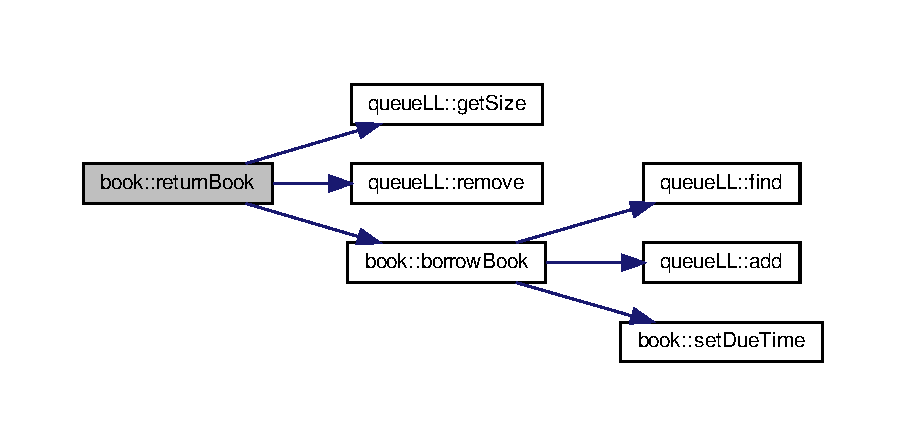
\includegraphics[width=350pt]{classbook_af11d02d9964b788986dc8e26d1cdf373_cgraph}
\end{center}
\end{figure}
Here is the caller graph for this function\+:
\nopagebreak
\begin{figure}[H]
\begin{center}
\leavevmode
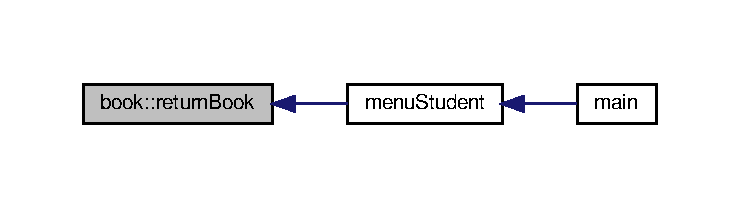
\includegraphics[width=350pt]{classbook_af11d02d9964b788986dc8e26d1cdf373_icgraph}
\end{center}
\end{figure}
\mbox{\Hypertarget{classbook_ab6da44e6c1680a8e802a14c2fcd20e78}\label{classbook_ab6da44e6c1680a8e802a14c2fcd20e78}} 
\index{book@{book}!set\+Author\+Name@{set\+Author\+Name}}
\index{set\+Author\+Name@{set\+Author\+Name}!book@{book}}
\subsubsection{\texorpdfstring{set\+Author\+Name()}{setAuthorName()}}
{\footnotesize\ttfamily void book\+::set\+Author\+Name (\begin{DoxyParamCaption}\item[{const std\+::string \&}]{author\+Name }\end{DoxyParamCaption})}

function sets the name of the author 
\begin{DoxyParams}{Parameters}
{\em author\+Name} & the name of the author \\
\hline
\end{DoxyParams}


Definition at line 42 of file Book.\+cpp.


\begin{DoxyCode}
42                                                     \{
43     this->\hyperlink{classbook_a21b2962c6227818732db27f12121b732}{authorName} = \hyperlink{classbook_a21b2962c6227818732db27f12121b732}{authorName};
44 \}
\end{DoxyCode}
\mbox{\Hypertarget{classbook_a7deed8c0520ef6f6b1dd5ebf9345cc72}\label{classbook_a7deed8c0520ef6f6b1dd5ebf9345cc72}} 
\index{book@{book}!set\+Borrowed@{set\+Borrowed}}
\index{set\+Borrowed@{set\+Borrowed}!book@{book}}
\subsubsection{\texorpdfstring{set\+Borrowed()}{setBorrowed()}}
{\footnotesize\ttfamily void book\+::set\+Borrowed (\begin{DoxyParamCaption}\item[{bool}]{borrowed }\end{DoxyParamCaption})}

function sets borrowed 
\begin{DoxyParams}{Parameters}
{\em borrowed} & shows if book is borrowed or not \\
\hline
\end{DoxyParams}


Definition at line 51 of file Book.\+cpp.


\begin{DoxyCode}
51                                     \{
52     this->\hyperlink{classbook_ab745520ed537e69bde6f2e3d7a103276}{borrowed} = \hyperlink{classbook_ab745520ed537e69bde6f2e3d7a103276}{borrowed};
53 \}
\end{DoxyCode}
\mbox{\Hypertarget{classbook_a61624bab2476a61fb2f27ebf7c8976e3}\label{classbook_a61624bab2476a61fb2f27ebf7c8976e3}} 
\index{book@{book}!set\+Due\+Time@{set\+Due\+Time}}
\index{set\+Due\+Time@{set\+Due\+Time}!book@{book}}
\subsubsection{\texorpdfstring{set\+Due\+Time()}{setDueTime()}}
{\footnotesize\ttfamily void book\+::set\+Due\+Time (\begin{DoxyParamCaption}{ }\end{DoxyParamCaption})}

function sets the due time 

Definition at line 59 of file Book.\+cpp.


\begin{DoxyCode}
59                       \{
60 
61      time\_t now = time( NULL);
62 
63      \hyperlink{classbook_abf72d9a32cdadee632df5a626dbe33b8}{due\_time} = *localtime( &now);
64 
65      \hyperlink{classbook_abf72d9a32cdadee632df5a626dbe33b8}{due\_time}.tm\_hour += \hyperlink{_book_8h_aded88185ac6dc121bc515c79c54a917a}{BORROW\_TIME};
66 \}
\end{DoxyCode}
Here is the caller graph for this function\+:
\nopagebreak
\begin{figure}[H]
\begin{center}
\leavevmode
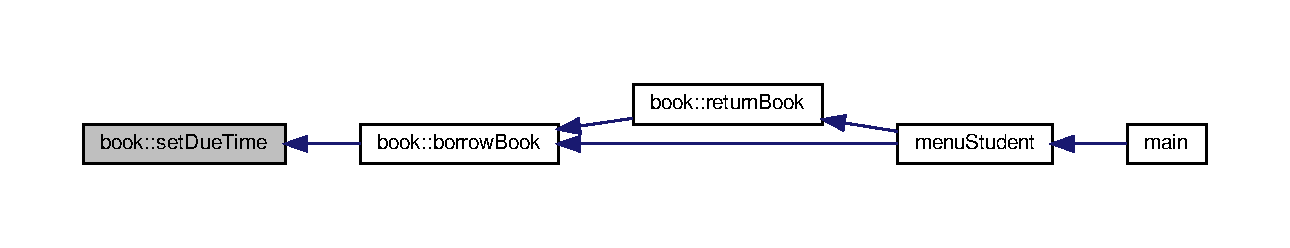
\includegraphics[width=350pt]{classbook_a61624bab2476a61fb2f27ebf7c8976e3_icgraph}
\end{center}
\end{figure}
\mbox{\Hypertarget{classbook_a40395f6b694a4c816bcf7a0ef279cf26}\label{classbook_a40395f6b694a4c816bcf7a0ef279cf26}} 
\index{book@{book}!set\+Name@{set\+Name}}
\index{set\+Name@{set\+Name}!book@{book}}
\subsubsection{\texorpdfstring{set\+Name()}{setName()}}
{\footnotesize\ttfamily void book\+::set\+Name (\begin{DoxyParamCaption}\item[{const std\+::string \&}]{name }\end{DoxyParamCaption})}

function sets the book name 
\begin{DoxyParams}{Parameters}
{\em name\+:the} & book name \\
\hline
\end{DoxyParams}


Definition at line 76 of file Book.\+cpp.


\begin{DoxyCode}
76                                         \{
77     this->\hyperlink{classbook_a5eabc1c1c5abff26997bec3d41f90d9e}{name} = \hyperlink{classbook_a5eabc1c1c5abff26997bec3d41f90d9e}{name};
78 \}
\end{DoxyCode}
\mbox{\Hypertarget{classbook_a458d26a8ddd01f69083a68eb68bf2181}\label{classbook_a458d26a8ddd01f69083a68eb68bf2181}} 
\index{book@{book}!to\+String@{to\+String}}
\index{to\+String@{to\+String}!book@{book}}
\subsubsection{\texorpdfstring{to\+String()}{toString()}}
{\footnotesize\ttfamily void book\+::to\+String (\begin{DoxyParamCaption}\item[{std\+::string \&}]{out }\end{DoxyParamCaption})}

function converts the book object to string 
\begin{DoxyParams}{Parameters}
{\em out} & the output string \\
\hline
\end{DoxyParams}


Definition at line 124 of file Book.\+cpp.


\begin{DoxyCode}
124                                    \{
125      std::string tmp= \hyperlink{classbook_ab745520ed537e69bde6f2e3d7a103276}{borrowed}?\textcolor{stringliteral}{"borrowed "}:\textcolor{stringliteral}{"not borrowed "};
126      time\_t t = mktime(&\hyperlink{classbook_abf72d9a32cdadee632df5a626dbe33b8}{due\_time});
127 \textcolor{comment}{//   std::string tmp2 = ctime(&t);}
128      std::string tmp2 = std::to\_string(t);
129      out = tmp2 +\textcolor{stringliteral}{" id="}+std::to\_string(\textcolor{keywordtype}{id}) + \textcolor{stringliteral}{" name="}+
130             \hyperlink{classbook_a5eabc1c1c5abff26997bec3d41f90d9e}{name}+ \textcolor{stringliteral}{" author\_name="}+\hyperlink{classbook_a21b2962c6227818732db27f12121b732}{authorName}+ \textcolor{stringliteral}{" "}+ tmp+\textcolor{stringliteral}{"\(\backslash\)n"};
131 \}
\end{DoxyCode}
Here is the caller graph for this function\+:
\nopagebreak
\begin{figure}[H]
\begin{center}
\leavevmode
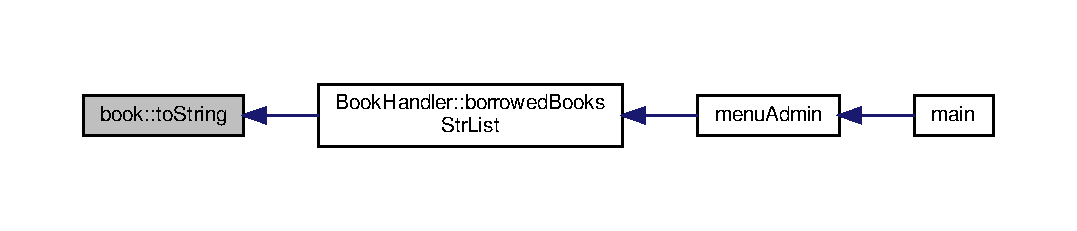
\includegraphics[width=350pt]{classbook_a458d26a8ddd01f69083a68eb68bf2181_icgraph}
\end{center}
\end{figure}


\subsection{Friends And Related Function Documentation}
\mbox{\Hypertarget{classbook_af7856e28b06865a9691d5c7a330633a4}\label{classbook_af7856e28b06865a9691d5c7a330633a4}} 
\index{book@{book}!operator"!=@{operator"!=}}
\index{operator"!=@{operator"!=}!book@{book}}
\subsubsection{\texorpdfstring{operator"!=}{operator!=}}
{\footnotesize\ttfamily bool operator!= (\begin{DoxyParamCaption}\item[{const \hyperlink{classbook}{book} \&}]{b1,  }\item[{const \hyperlink{classbook}{book} \&}]{b2 }\end{DoxyParamCaption})\hspace{0.3cm}{\ttfamily [friend]}}

function overloads operator != (not equal) 
\begin{DoxyParams}{Parameters}
{\em b1} & first book object \\
\hline
{\em b2} & second book object \\
\hline
\end{DoxyParams}
\begin{DoxyReturn}{Returns}

\end{DoxyReturn}


Definition at line 156 of file Book.\+cpp.


\begin{DoxyCode}
156                                                  \{
157     \textcolor{keywordflow}{if}(b1.\hyperlink{classbook_ad8bf54b50c72af3827823c04d724d824}{id}!=b2.\hyperlink{classbook_ad8bf54b50c72af3827823c04d724d824}{id} || b1.\hyperlink{classbook_a5eabc1c1c5abff26997bec3d41f90d9e}{name}!=b2.\hyperlink{classbook_a5eabc1c1c5abff26997bec3d41f90d9e}{name} || b1.\hyperlink{classbook_a21b2962c6227818732db27f12121b732}{authorName}!=b2.
      \hyperlink{classbook_a21b2962c6227818732db27f12121b732}{authorName})
158         \textcolor{keywordflow}{return} \textcolor{keyword}{true};
159     \textcolor{keywordflow}{else}
160         \textcolor{keywordflow}{return} \textcolor{keyword}{false};
161 \}
\end{DoxyCode}
\mbox{\Hypertarget{classbook_a3d386e1f8255c6b62d9858fb8ff41c86}\label{classbook_a3d386e1f8255c6b62d9858fb8ff41c86}} 
\index{book@{book}!operator$<$@{operator$<$}}
\index{operator$<$@{operator$<$}!book@{book}}
\subsubsection{\texorpdfstring{operator$<$}{operator<}}
{\footnotesize\ttfamily bool operator$<$ (\begin{DoxyParamCaption}\item[{\hyperlink{classbook}{book} \&}]{b1,  }\item[{\hyperlink{classbook}{book} \&}]{b2 }\end{DoxyParamCaption})\hspace{0.3cm}{\ttfamily [friend]}}

overload operator $<$ 
\begin{DoxyParams}{Parameters}
{\em b1} & first book object \\
\hline
{\em b2} & first book object \\
\hline
\end{DoxyParams}
\begin{DoxyReturn}{Returns}
true, if due time b1 is smaller than due time b2 
\end{DoxyReturn}


Definition at line 163 of file Book.\+cpp.


\begin{DoxyCode}
163                                       \{
164     time\_t t1 = mktime(&(b1.\hyperlink{classbook_abf72d9a32cdadee632df5a626dbe33b8}{due\_time}));
165     time\_t t2 = mktime(&(b2.\hyperlink{classbook_abf72d9a32cdadee632df5a626dbe33b8}{due\_time}));
166     \textcolor{keywordtype}{double} diffSecs = difftime(t1, t2);
167     \textcolor{keywordflow}{if}(diffSecs<0 )
168         \textcolor{keywordflow}{return} \textcolor{keyword}{true};
169     \textcolor{keywordflow}{else}
170         \textcolor{keywordflow}{return} \textcolor{keyword}{false};
171 \}
\end{DoxyCode}
\mbox{\Hypertarget{classbook_a9bd0243ea50c5b8c37ed0d5527f24177}\label{classbook_a9bd0243ea50c5b8c37ed0d5527f24177}} 
\index{book@{book}!operator$<$$<$@{operator$<$$<$}}
\index{operator$<$$<$@{operator$<$$<$}!book@{book}}
\subsubsection{\texorpdfstring{operator$<$$<$}{operator<<}}
{\footnotesize\ttfamily std\+::ostream\& operator$<$$<$ (\begin{DoxyParamCaption}\item[{std\+::ostream \&}]{out,  }\item[{const \hyperlink{classbook}{book} \&}]{b }\end{DoxyParamCaption})\hspace{0.3cm}{\ttfamily [friend]}}

function overloads operator $<$$<$ 
\begin{DoxyParams}{Parameters}
{\em out} & output stream \\
\hline
{\em b} & book object \\
\hline
\end{DoxyParams}
\begin{DoxyReturn}{Returns}

\end{DoxyReturn}


Definition at line 133 of file Book.\+cpp.


\begin{DoxyCode}
133                                                         \{
134      std::string tmp= b.\hyperlink{classbook_ab745520ed537e69bde6f2e3d7a103276}{borrowed}?\textcolor{stringliteral}{"borrowed "}:\textcolor{stringliteral}{"not borrowed "};
135      \textcolor{keywordflow}{if}(b.\hyperlink{classbook_a40ce04fcfbf99ffdbe7a4e1463588ee5}{waitingStudentId}->\hyperlink{classqueue_l_l_a8969feebcb563f0b489bc112422b9563}{getSize}()>0)
136          \textcolor{keywordflow}{return} out <<\textcolor{stringliteral}{"BOOK id="}<< b.\hyperlink{classbook_ad8bf54b50c72af3827823c04d724d824}{id} << \textcolor{stringliteral}{" name="} << b.\hyperlink{classbook_a5eabc1c1c5abff26997bec3d41f90d9e}{name} << \textcolor{stringliteral}{" author="}
137                  << b.\hyperlink{classbook_a21b2962c6227818732db27f12121b732}{authorName} << \textcolor{stringliteral}{" "}<<tmp << \textcolor{stringliteral}{" due date="}
138                  << b.\hyperlink{classbook_abf72d9a32cdadee632df5a626dbe33b8}{due\_time}.tm\_year<<\textcolor{stringliteral}{"-"}<< b.\hyperlink{classbook_abf72d9a32cdadee632df5a626dbe33b8}{due\_time}.tm\_mon<<\textcolor{stringliteral}{"-"}
139                  << b.\hyperlink{classbook_abf72d9a32cdadee632df5a626dbe33b8}{due\_time}.tm\_mday<<\textcolor{stringliteral}{" "}<< b.\hyperlink{classbook_abf72d9a32cdadee632df5a626dbe33b8}{due\_time}.tm\_hour<<\textcolor{stringliteral}{":"}
140                  << b.\hyperlink{classbook_abf72d9a32cdadee632df5a626dbe33b8}{due\_time}.tm\_min<< \textcolor{stringliteral}{":"}<< b.\hyperlink{classbook_abf72d9a32cdadee632df5a626dbe33b8}{due\_time}.tm\_sec
141                  <<\textcolor{stringliteral}{" waiting students' id="}<< *(b.\hyperlink{classbook_a40ce04fcfbf99ffdbe7a4e1463588ee5}{waitingStudentId})<<\textcolor{stringliteral}{"\(\backslash\)n"};
142      \textcolor{keywordflow}{else}\{
143          \textcolor{keywordflow}{if}( b.\hyperlink{classbook_ab745520ed537e69bde6f2e3d7a103276}{borrowed})
144              \textcolor{keywordflow}{return} out <<\textcolor{stringliteral}{"BOOK id="}<< b.\hyperlink{classbook_ad8bf54b50c72af3827823c04d724d824}{id} << \textcolor{stringliteral}{" name="} << b.\hyperlink{classbook_a5eabc1c1c5abff26997bec3d41f90d9e}{name} << \textcolor{stringliteral}{" author="}
145                      << b.\hyperlink{classbook_a21b2962c6227818732db27f12121b732}{authorName} << \textcolor{stringliteral}{" "}<< tmp << \textcolor{stringliteral}{" due date="}
146                      << b.\hyperlink{classbook_abf72d9a32cdadee632df5a626dbe33b8}{due\_time}.tm\_year<<\textcolor{stringliteral}{"-"}<< b.\hyperlink{classbook_abf72d9a32cdadee632df5a626dbe33b8}{due\_time}.tm\_mon<<\textcolor{stringliteral}{"-"}
147                      << b.\hyperlink{classbook_abf72d9a32cdadee632df5a626dbe33b8}{due\_time}.tm\_mday<<\textcolor{stringliteral}{" "}<< b.\hyperlink{classbook_abf72d9a32cdadee632df5a626dbe33b8}{due\_time}.tm\_hour<<\textcolor{stringliteral}{":"}
148                      << b.\hyperlink{classbook_abf72d9a32cdadee632df5a626dbe33b8}{due\_time}.tm\_min<< \textcolor{stringliteral}{":"}<< b.\hyperlink{classbook_abf72d9a32cdadee632df5a626dbe33b8}{due\_time}.tm\_sec <<\textcolor{stringliteral}{"\(\backslash\)n"};
149          \textcolor{keywordflow}{else}
150              \textcolor{keywordflow}{return} out <<\textcolor{stringliteral}{"BOOK id="}<< b.\hyperlink{classbook_ad8bf54b50c72af3827823c04d724d824}{id} << \textcolor{stringliteral}{" name="} << b.\hyperlink{classbook_a5eabc1c1c5abff26997bec3d41f90d9e}{name} << \textcolor{stringliteral}{" author="}
151                                  << b.\hyperlink{classbook_a21b2962c6227818732db27f12121b732}{authorName} << \textcolor{stringliteral}{" "}<< tmp<<\textcolor{stringliteral}{"\(\backslash\)n"};
152      \}
153 \}
\end{DoxyCode}


\subsection{Member Data Documentation}
\mbox{\Hypertarget{classbook_a21b2962c6227818732db27f12121b732}\label{classbook_a21b2962c6227818732db27f12121b732}} 
\index{book@{book}!author\+Name@{author\+Name}}
\index{author\+Name@{author\+Name}!book@{book}}
\subsubsection{\texorpdfstring{author\+Name}{authorName}}
{\footnotesize\ttfamily std\+::string book\+::author\+Name\hspace{0.3cm}{\ttfamily [private]}}

author name of the book 

Definition at line 156 of file Book.\+h.

\mbox{\Hypertarget{classbook_ab745520ed537e69bde6f2e3d7a103276}\label{classbook_ab745520ed537e69bde6f2e3d7a103276}} 
\index{book@{book}!borrowed@{borrowed}}
\index{borrowed@{borrowed}!book@{book}}
\subsubsection{\texorpdfstring{borrowed}{borrowed}}
{\footnotesize\ttfamily bool book\+::borrowed\hspace{0.3cm}{\ttfamily [private]}}

if book is borrowed or not 

Definition at line 160 of file Book.\+h.

\mbox{\Hypertarget{classbook_afa5350900be6a34d8301a57d6db54df5}\label{classbook_afa5350900be6a34d8301a57d6db54df5}} 
\index{book@{book}!borrowed\+By\+Student@{borrowed\+By\+Student}}
\index{borrowed\+By\+Student@{borrowed\+By\+Student}!book@{book}}
\subsubsection{\texorpdfstring{borrowed\+By\+Student}{borrowedByStudent}}
{\footnotesize\ttfamily int book\+::borrowed\+By\+Student\hspace{0.3cm}{\ttfamily [private]}}

student id that borrowed the book 

Definition at line 164 of file Book.\+h.

\mbox{\Hypertarget{classbook_abf72d9a32cdadee632df5a626dbe33b8}\label{classbook_abf72d9a32cdadee632df5a626dbe33b8}} 
\index{book@{book}!due\+\_\+time@{due\+\_\+time}}
\index{due\+\_\+time@{due\+\_\+time}!book@{book}}
\subsubsection{\texorpdfstring{due\+\_\+time}{due\_time}}
{\footnotesize\ttfamily tm book\+::due\+\_\+time\hspace{0.3cm}{\ttfamily [private]}}

due time of returning the book 

Definition at line 168 of file Book.\+h.

\mbox{\Hypertarget{classbook_ad8bf54b50c72af3827823c04d724d824}\label{classbook_ad8bf54b50c72af3827823c04d724d824}} 
\index{book@{book}!id@{id}}
\index{id@{id}!book@{book}}
\subsubsection{\texorpdfstring{id}{id}}
{\footnotesize\ttfamily int book\+::id\hspace{0.3cm}{\ttfamily [private]}}

id of the book 

Definition at line 148 of file Book.\+h.

\mbox{\Hypertarget{classbook_a5eabc1c1c5abff26997bec3d41f90d9e}\label{classbook_a5eabc1c1c5abff26997bec3d41f90d9e}} 
\index{book@{book}!name@{name}}
\index{name@{name}!book@{book}}
\subsubsection{\texorpdfstring{name}{name}}
{\footnotesize\ttfamily std\+::string book\+::name\hspace{0.3cm}{\ttfamily [private]}}

name of the book 

Definition at line 152 of file Book.\+h.

\mbox{\Hypertarget{classbook_a40ce04fcfbf99ffdbe7a4e1463588ee5}\label{classbook_a40ce04fcfbf99ffdbe7a4e1463588ee5}} 
\index{book@{book}!waiting\+Student\+Id@{waiting\+Student\+Id}}
\index{waiting\+Student\+Id@{waiting\+Student\+Id}!book@{book}}
\subsubsection{\texorpdfstring{waiting\+Student\+Id}{waitingStudentId}}
{\footnotesize\ttfamily \hyperlink{classqueue_l_l}{queue\+LL}$<$int$>$$\ast$ book\+::waiting\+Student\+Id\hspace{0.3cm}{\ttfamily [private]}}

waiting list of students\textquotesingle{} id who want to borrow the book 

Definition at line 172 of file Book.\+h.



The documentation for this class was generated from the following files\+:\begin{DoxyCompactItemize}
\item 
src/\hyperlink{_book_8h}{Book.\+h}\item 
src/\hyperlink{_book_8cpp}{Book.\+cpp}\end{DoxyCompactItemize}

\hypertarget{class_book_handler}{}\section{Book\+Handler Class Reference}
\label{class_book_handler}\index{Book\+Handler@{Book\+Handler}}


{\ttfamily \#include $<$Book\+Handler.\+h$>$}



Collaboration diagram for Book\+Handler\+:
\nopagebreak
\begin{figure}[H]
\begin{center}
\leavevmode
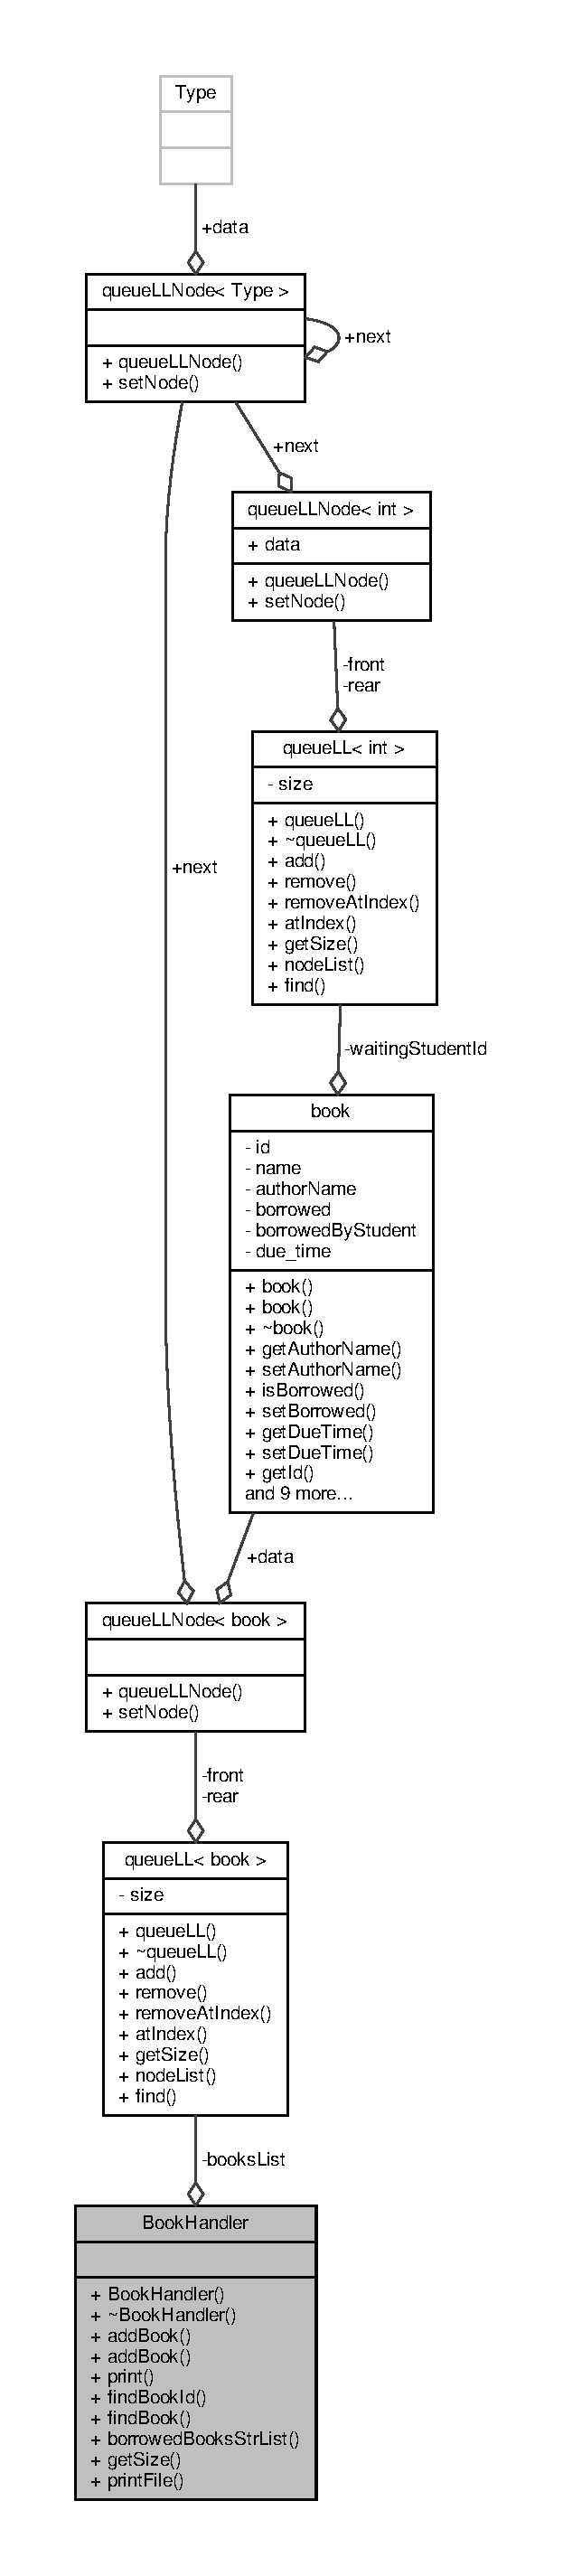
\includegraphics[height=550pt]{class_book_handler__coll__graph}
\end{center}
\end{figure}
\subsection*{Public Member Functions}
\begin{DoxyCompactItemize}
\item 
\hyperlink{class_book_handler_a73362998148ff419f5dccd629f858832}{Book\+Handler} ()
\item 
virtual \hyperlink{class_book_handler_afd60e561a18f17d087da3c8b04d0c842}{$\sim$\+Book\+Handler} ()
\item 
void \hyperlink{class_book_handler_a29517e8c55796a94f29c48d6971e9f1d}{add\+Book} (std\+::string name, std\+::string auth\+Name)
\item 
void \hyperlink{class_book_handler_aac102920daa87a20f3e169f9c3cbc33b}{add\+Book} (\hyperlink{classbook}{book} $\ast$temp)
\item 
void \hyperlink{class_book_handler_ac6e2d4211b55e636348daaa9253a2d12}{print} ()
\item 
\hyperlink{classbook}{book} $\ast$ \hyperlink{class_book_handler_ae82abc7349e19e59cd6f3cb23c7928fa}{find\+Book\+Id} (int index)
\item 
\hyperlink{classbook}{book} $\ast$ \hyperlink{class_book_handler_aab461b060b38d51586ed043143b4bc68}{find\+Book} (\hyperlink{classbook}{book} \&temp)
\item 
void \hyperlink{class_book_handler_ac0274027fa9375870ffb08fbb6377a7d}{borrowed\+Books\+Str\+List} (std\+::string $\ast$result, int \&borrowed\+Books\+Size)
\item 
int \hyperlink{class_book_handler_a2939194b5d19618d5a69743b4c0dc240}{get\+Size} ()
\item 
void \hyperlink{class_book_handler_a6794f0f693ff3048df64a5b254c183af}{print\+File} (std\+::ofstream \&ou\+File)
\end{DoxyCompactItemize}
\subsection*{Private Attributes}
\begin{DoxyCompactItemize}
\item 
\hyperlink{classqueue_l_l}{queue\+LL}$<$ \hyperlink{classbook}{book} $>$ $\ast$ \hyperlink{class_book_handler_a13a6c78422b3ad7acd5ebdb9555a0286}{books\+List}
\end{DoxyCompactItemize}


\subsection{Detailed Description}
Class handles the list of the books 

Definition at line 18 of file Book\+Handler.\+h.



\subsection{Constructor \& Destructor Documentation}
\mbox{\Hypertarget{class_book_handler_a73362998148ff419f5dccd629f858832}\label{class_book_handler_a73362998148ff419f5dccd629f858832}} 
\index{Book\+Handler@{Book\+Handler}!Book\+Handler@{Book\+Handler}}
\index{Book\+Handler@{Book\+Handler}!Book\+Handler@{Book\+Handler}}
\subsubsection{\texorpdfstring{Book\+Handler()}{BookHandler()}}
{\footnotesize\ttfamily Book\+Handler\+::\+Book\+Handler (\begin{DoxyParamCaption}{ }\end{DoxyParamCaption})}

constructor function 

Definition at line 10 of file Book\+Handler.\+cpp.


\begin{DoxyCode}
10                          \{
11     \hyperlink{class_book_handler_a13a6c78422b3ad7acd5ebdb9555a0286}{booksList} = \textcolor{keyword}{new} \hyperlink{classqueue_l_l}{queueLL<book>}();
12 \}
\end{DoxyCode}
\mbox{\Hypertarget{class_book_handler_afd60e561a18f17d087da3c8b04d0c842}\label{class_book_handler_afd60e561a18f17d087da3c8b04d0c842}} 
\index{Book\+Handler@{Book\+Handler}!````~Book\+Handler@{$\sim$\+Book\+Handler}}
\index{````~Book\+Handler@{$\sim$\+Book\+Handler}!Book\+Handler@{Book\+Handler}}
\subsubsection{\texorpdfstring{$\sim$\+Book\+Handler()}{~BookHandler()}}
{\footnotesize\ttfamily Book\+Handler\+::$\sim$\+Book\+Handler (\begin{DoxyParamCaption}{ }\end{DoxyParamCaption})\hspace{0.3cm}{\ttfamily [virtual]}}

destructor function 

Definition at line 14 of file Book\+Handler.\+cpp.


\begin{DoxyCode}
14                           \{
15     \textcolor{keyword}{delete}(\hyperlink{class_book_handler_a13a6c78422b3ad7acd5ebdb9555a0286}{booksList});
16 \}
\end{DoxyCode}


\subsection{Member Function Documentation}
\mbox{\Hypertarget{class_book_handler_a29517e8c55796a94f29c48d6971e9f1d}\label{class_book_handler_a29517e8c55796a94f29c48d6971e9f1d}} 
\index{Book\+Handler@{Book\+Handler}!add\+Book@{add\+Book}}
\index{add\+Book@{add\+Book}!Book\+Handler@{Book\+Handler}}
\subsubsection{\texorpdfstring{add\+Book()}{addBook()}\hspace{0.1cm}{\footnotesize\ttfamily [1/2]}}
{\footnotesize\ttfamily void Book\+Handler\+::add\+Book (\begin{DoxyParamCaption}\item[{std\+::string}]{name,  }\item[{std\+::string}]{auth\+Name }\end{DoxyParamCaption})}

function to add a book to the list of the books 
\begin{DoxyParams}{Parameters}
{\em name} & book name \\
\hline
{\em auth\+Name} & author name of the book \\
\hline
\end{DoxyParams}


Definition at line 18 of file Book\+Handler.\+cpp.


\begin{DoxyCode}
18                                                             \{
19     \hyperlink{classbook}{book} * temp = \textcolor{keyword}{new} \hyperlink{classbook}{book}(name, authName);
20     \hyperlink{class_book_handler_a13a6c78422b3ad7acd5ebdb9555a0286}{booksList}->\hyperlink{classqueue_l_l_adcbcc26433da2c9d17b6cf0802d1d7d2}{add}(temp);
21 \}
\end{DoxyCode}
Here is the call graph for this function\+:
\nopagebreak
\begin{figure}[H]
\begin{center}
\leavevmode
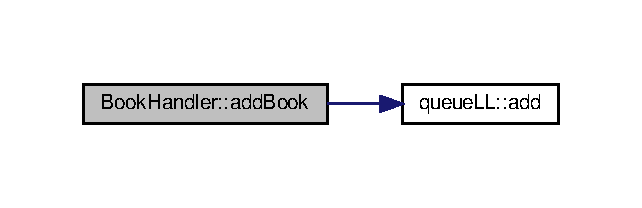
\includegraphics[width=308pt]{class_book_handler_a29517e8c55796a94f29c48d6971e9f1d_cgraph}
\end{center}
\end{figure}
Here is the caller graph for this function\+:
\nopagebreak
\begin{figure}[H]
\begin{center}
\leavevmode
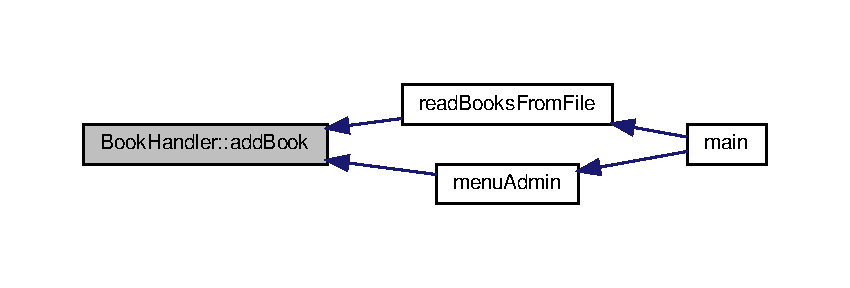
\includegraphics[width=350pt]{class_book_handler_a29517e8c55796a94f29c48d6971e9f1d_icgraph}
\end{center}
\end{figure}
\mbox{\Hypertarget{class_book_handler_aac102920daa87a20f3e169f9c3cbc33b}\label{class_book_handler_aac102920daa87a20f3e169f9c3cbc33b}} 
\index{Book\+Handler@{Book\+Handler}!add\+Book@{add\+Book}}
\index{add\+Book@{add\+Book}!Book\+Handler@{Book\+Handler}}
\subsubsection{\texorpdfstring{add\+Book()}{addBook()}\hspace{0.1cm}{\footnotesize\ttfamily [2/2]}}
{\footnotesize\ttfamily void Book\+Handler\+::add\+Book (\begin{DoxyParamCaption}\item[{\hyperlink{classbook}{book} $\ast$}]{temp }\end{DoxyParamCaption})}

function to add a book to the list of the books 
\begin{DoxyParams}{Parameters}
{\em temp} & book object \\
\hline
\end{DoxyParams}


Definition at line 22 of file Book\+Handler.\+cpp.


\begin{DoxyCode}
22                                      \{
23     \hyperlink{class_book_handler_a13a6c78422b3ad7acd5ebdb9555a0286}{booksList}->\hyperlink{classqueue_l_l_adcbcc26433da2c9d17b6cf0802d1d7d2}{add}(temp);
24 \}
\end{DoxyCode}
Here is the call graph for this function\+:
\nopagebreak
\begin{figure}[H]
\begin{center}
\leavevmode
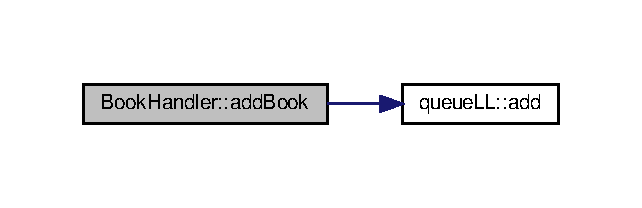
\includegraphics[width=308pt]{class_book_handler_aac102920daa87a20f3e169f9c3cbc33b_cgraph}
\end{center}
\end{figure}
\mbox{\Hypertarget{class_book_handler_ac0274027fa9375870ffb08fbb6377a7d}\label{class_book_handler_ac0274027fa9375870ffb08fbb6377a7d}} 
\index{Book\+Handler@{Book\+Handler}!borrowed\+Books\+Str\+List@{borrowed\+Books\+Str\+List}}
\index{borrowed\+Books\+Str\+List@{borrowed\+Books\+Str\+List}!Book\+Handler@{Book\+Handler}}
\subsubsection{\texorpdfstring{borrowed\+Books\+Str\+List()}{borrowedBooksStrList()}}
{\footnotesize\ttfamily void Book\+Handler\+::borrowed\+Books\+Str\+List (\begin{DoxyParamCaption}\item[{std\+::string $\ast$}]{result,  }\item[{int \&}]{borrowed\+Books\+Size }\end{DoxyParamCaption})}

function to make a list of the borrowed books between all the books in the list 
\begin{DoxyParams}{Parameters}
{\em result} & string list of the borrowed books \\
\hline
{\em borrowed\+Books\+Size} & size of the string list of the borrowed books \\
\hline
\end{DoxyParams}


Definition at line 70 of file Book\+Handler.\+cpp.


\begin{DoxyCode}
70                                                                                   \{
71     \hyperlink{classbook}{book} ** list = \hyperlink{class_book_handler_a13a6c78422b3ad7acd5ebdb9555a0286}{booksList}->\hyperlink{classqueue_l_l_ae9a479b9463f51c5148dd80b68335d32}{nodeList}();
72     \textcolor{keywordtype}{int} c=0;
73     \textcolor{keywordflow}{for}(\textcolor{keywordtype}{int} i=0; i<\hyperlink{class_book_handler_a13a6c78422b3ad7acd5ebdb9555a0286}{booksList}->\hyperlink{classqueue_l_l_a8969feebcb563f0b489bc112422b9563}{getSize}(); i++)\{
74         \textcolor{keywordflow}{if}(list[i]->isBorrowed())\{
75             std::string temp ;
76             list[i]->\hyperlink{classbook_a458d26a8ddd01f69083a68eb68bf2181}{toString}(temp);
77             result[c++]=temp;
78         \}
79     \}
80     borrowedBooksSize = c;
81 \}
\end{DoxyCode}
Here is the call graph for this function\+:
\nopagebreak
\begin{figure}[H]
\begin{center}
\leavevmode
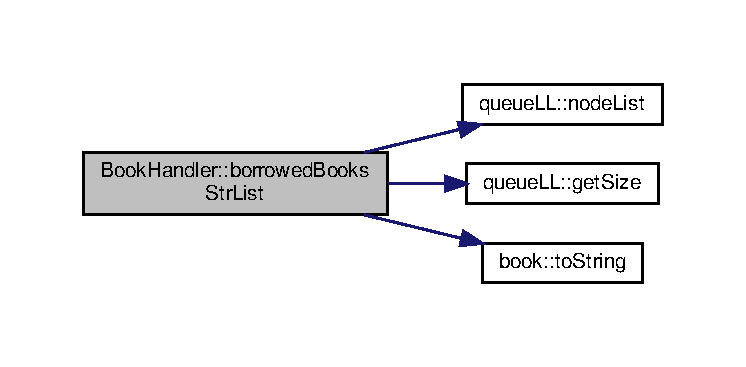
\includegraphics[width=350pt]{class_book_handler_ac0274027fa9375870ffb08fbb6377a7d_cgraph}
\end{center}
\end{figure}
Here is the caller graph for this function\+:
\nopagebreak
\begin{figure}[H]
\begin{center}
\leavevmode
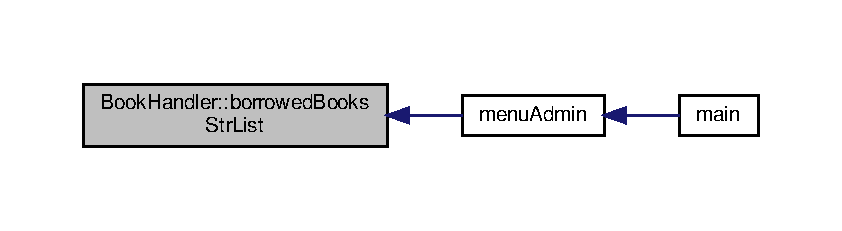
\includegraphics[width=350pt]{class_book_handler_ac0274027fa9375870ffb08fbb6377a7d_icgraph}
\end{center}
\end{figure}
\mbox{\Hypertarget{class_book_handler_aab461b060b38d51586ed043143b4bc68}\label{class_book_handler_aab461b060b38d51586ed043143b4bc68}} 
\index{Book\+Handler@{Book\+Handler}!find\+Book@{find\+Book}}
\index{find\+Book@{find\+Book}!Book\+Handler@{Book\+Handler}}
\subsubsection{\texorpdfstring{find\+Book()}{findBook()}}
{\footnotesize\ttfamily \hyperlink{classbook}{book} $\ast$ Book\+Handler\+::find\+Book (\begin{DoxyParamCaption}\item[{\hyperlink{classbook}{book} \&}]{temp }\end{DoxyParamCaption})}

function to find book object among the books list 
\begin{DoxyParams}{Parameters}
{\em temp} & book object \\
\hline
\end{DoxyParams}
\begin{DoxyReturn}{Returns}
\+: pointer to the found book 
\end{DoxyReturn}


Definition at line 51 of file Book\+Handler.\+cpp.


\begin{DoxyCode}
51                                         \{
52     \hyperlink{classbook}{book} ** list = \hyperlink{class_book_handler_a13a6c78422b3ad7acd5ebdb9555a0286}{booksList}->\hyperlink{classqueue_l_l_ae9a479b9463f51c5148dd80b68335d32}{nodeList}();
53     \textcolor{keywordflow}{for}(\textcolor{keywordtype}{int} i=0; i<\hyperlink{class_book_handler_a13a6c78422b3ad7acd5ebdb9555a0286}{booksList}->\hyperlink{classqueue_l_l_a8969feebcb563f0b489bc112422b9563}{getSize}(); i++)\{
54         \textcolor{keywordflow}{if}(!(*list[i]!=temp))\{
55             \textcolor{keywordflow}{return} list[i];
56         \}
57     \}
58     \textcolor{keywordflow}{return} NULL;
59 \}
\end{DoxyCode}
Here is the call graph for this function\+:
\nopagebreak
\begin{figure}[H]
\begin{center}
\leavevmode
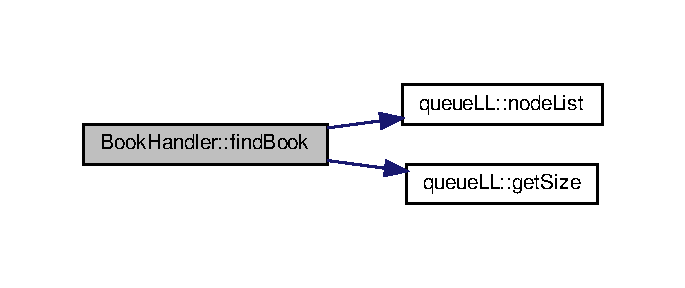
\includegraphics[width=329pt]{class_book_handler_aab461b060b38d51586ed043143b4bc68_cgraph}
\end{center}
\end{figure}
Here is the caller graph for this function\+:
\nopagebreak
\begin{figure}[H]
\begin{center}
\leavevmode
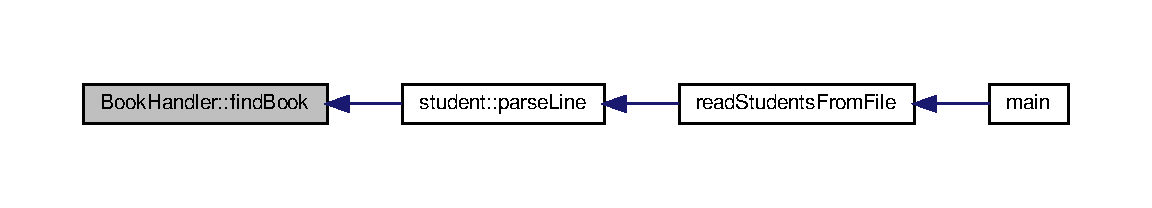
\includegraphics[width=350pt]{class_book_handler_aab461b060b38d51586ed043143b4bc68_icgraph}
\end{center}
\end{figure}
\mbox{\Hypertarget{class_book_handler_ae82abc7349e19e59cd6f3cb23c7928fa}\label{class_book_handler_ae82abc7349e19e59cd6f3cb23c7928fa}} 
\index{Book\+Handler@{Book\+Handler}!find\+Book\+Id@{find\+Book\+Id}}
\index{find\+Book\+Id@{find\+Book\+Id}!Book\+Handler@{Book\+Handler}}
\subsubsection{\texorpdfstring{find\+Book\+Id()}{findBookId()}}
{\footnotesize\ttfamily \hyperlink{classbook}{book} $\ast$ Book\+Handler\+::find\+Book\+Id (\begin{DoxyParamCaption}\item[{int}]{index }\end{DoxyParamCaption})}

function to find id of the book at location index of the books list 
\begin{DoxyParams}{Parameters}
{\em index} & \\
\hline
\end{DoxyParams}
\begin{DoxyReturn}{Returns}
\+: pointer to the found book 
\end{DoxyReturn}


Definition at line 42 of file Book\+Handler.\+cpp.


\begin{DoxyCode}
42                                         \{
43     \hyperlink{classbook}{book} ** list = \hyperlink{class_book_handler_a13a6c78422b3ad7acd5ebdb9555a0286}{booksList}->\hyperlink{classqueue_l_l_ae9a479b9463f51c5148dd80b68335d32}{nodeList}();
44     \textcolor{keywordflow}{for}(\textcolor{keywordtype}{int} i=0; i<\hyperlink{class_book_handler_a13a6c78422b3ad7acd5ebdb9555a0286}{booksList}->\hyperlink{classqueue_l_l_a8969feebcb563f0b489bc112422b9563}{getSize}(); i++)\{
45         \textcolor{keywordflow}{if}(list[i]->getId()==index)\{
46             \textcolor{keywordflow}{return} list[i];
47         \}
48     \}
49     \textcolor{keywordflow}{return} NULL;
50 \}
\end{DoxyCode}
Here is the call graph for this function\+:
\nopagebreak
\begin{figure}[H]
\begin{center}
\leavevmode
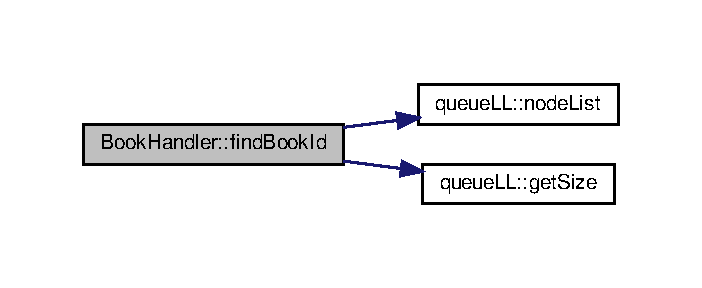
\includegraphics[width=337pt]{class_book_handler_ae82abc7349e19e59cd6f3cb23c7928fa_cgraph}
\end{center}
\end{figure}
Here is the caller graph for this function\+:
\nopagebreak
\begin{figure}[H]
\begin{center}
\leavevmode
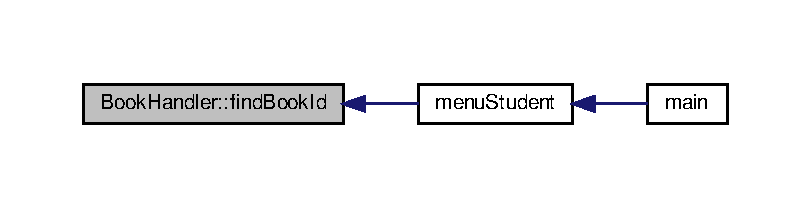
\includegraphics[width=350pt]{class_book_handler_ae82abc7349e19e59cd6f3cb23c7928fa_icgraph}
\end{center}
\end{figure}
\mbox{\Hypertarget{class_book_handler_a2939194b5d19618d5a69743b4c0dc240}\label{class_book_handler_a2939194b5d19618d5a69743b4c0dc240}} 
\index{Book\+Handler@{Book\+Handler}!get\+Size@{get\+Size}}
\index{get\+Size@{get\+Size}!Book\+Handler@{Book\+Handler}}
\subsubsection{\texorpdfstring{get\+Size()}{getSize()}}
{\footnotesize\ttfamily int Book\+Handler\+::get\+Size (\begin{DoxyParamCaption}{ }\end{DoxyParamCaption})}

function to return size of the books list \begin{DoxyReturn}{Returns}

\end{DoxyReturn}


Definition at line 83 of file Book\+Handler.\+cpp.


\begin{DoxyCode}
83                          \{
84     \textcolor{keywordflow}{return} \hyperlink{class_book_handler_a13a6c78422b3ad7acd5ebdb9555a0286}{booksList}->\hyperlink{classqueue_l_l_a8969feebcb563f0b489bc112422b9563}{getSize}();
85 \}
\end{DoxyCode}
Here is the call graph for this function\+:
\nopagebreak
\begin{figure}[H]
\begin{center}
\leavevmode
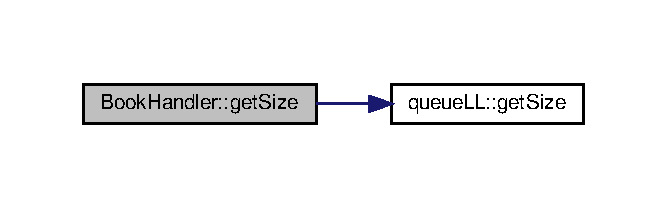
\includegraphics[width=320pt]{class_book_handler_a2939194b5d19618d5a69743b4c0dc240_cgraph}
\end{center}
\end{figure}
Here is the caller graph for this function\+:
\nopagebreak
\begin{figure}[H]
\begin{center}
\leavevmode
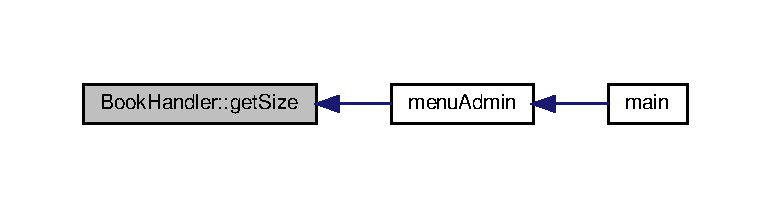
\includegraphics[width=350pt]{class_book_handler_a2939194b5d19618d5a69743b4c0dc240_icgraph}
\end{center}
\end{figure}
\mbox{\Hypertarget{class_book_handler_ac6e2d4211b55e636348daaa9253a2d12}\label{class_book_handler_ac6e2d4211b55e636348daaa9253a2d12}} 
\index{Book\+Handler@{Book\+Handler}!print@{print}}
\index{print@{print}!Book\+Handler@{Book\+Handler}}
\subsubsection{\texorpdfstring{print()}{print()}}
{\footnotesize\ttfamily void Book\+Handler\+::print (\begin{DoxyParamCaption}{ }\end{DoxyParamCaption})}

function to print the list of the books 

Definition at line 26 of file Book\+Handler.\+cpp.


\begin{DoxyCode}
26                         \{
27     \textcolor{keywordflow}{if}(\hyperlink{class_book_handler_a13a6c78422b3ad7acd5ebdb9555a0286}{booksList}->\hyperlink{classqueue_l_l_a8969feebcb563f0b489bc112422b9563}{getSize}() == 0)\{
28         std::cout<<\textcolor{stringliteral}{"No student is added to the tree"};
29     \}
30     \textcolor{keywordflow}{else} \{
31         std::cout<<*\hyperlink{class_book_handler_a13a6c78422b3ad7acd5ebdb9555a0286}{booksList};
32     \}
33 \}
\end{DoxyCode}
Here is the call graph for this function\+:
\nopagebreak
\begin{figure}[H]
\begin{center}
\leavevmode
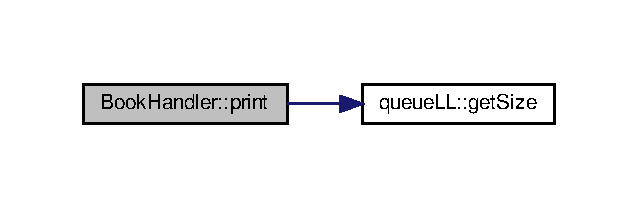
\includegraphics[width=306pt]{class_book_handler_ac6e2d4211b55e636348daaa9253a2d12_cgraph}
\end{center}
\end{figure}
Here is the caller graph for this function\+:
\nopagebreak
\begin{figure}[H]
\begin{center}
\leavevmode
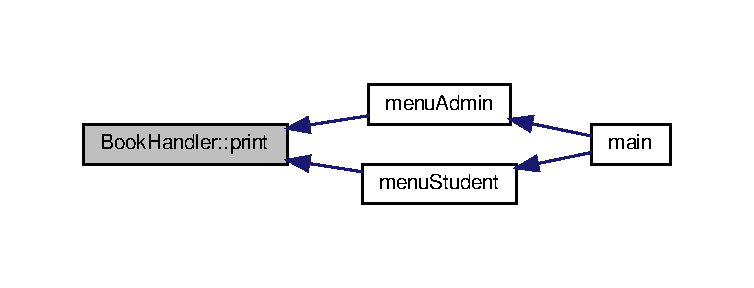
\includegraphics[width=350pt]{class_book_handler_ac6e2d4211b55e636348daaa9253a2d12_icgraph}
\end{center}
\end{figure}
\mbox{\Hypertarget{class_book_handler_a6794f0f693ff3048df64a5b254c183af}\label{class_book_handler_a6794f0f693ff3048df64a5b254c183af}} 
\index{Book\+Handler@{Book\+Handler}!print\+File@{print\+File}}
\index{print\+File@{print\+File}!Book\+Handler@{Book\+Handler}}
\subsubsection{\texorpdfstring{print\+File()}{printFile()}}
{\footnotesize\ttfamily void Book\+Handler\+::print\+File (\begin{DoxyParamCaption}\item[{std\+::ofstream \&}]{ou\+File }\end{DoxyParamCaption})}

function to print the list of the books to the file 

Definition at line 34 of file Book\+Handler.\+cpp.


\begin{DoxyCode}
34                                                \{
35     \hyperlink{classbook}{book} ** list = \hyperlink{class_book_handler_a13a6c78422b3ad7acd5ebdb9555a0286}{booksList}->\hyperlink{classqueue_l_l_ae9a479b9463f51c5148dd80b68335d32}{nodeList}();
36     \textcolor{keywordflow}{for}(\textcolor{keywordtype}{int} i=0; i<\hyperlink{class_book_handler_a13a6c78422b3ad7acd5ebdb9555a0286}{booksList}->\hyperlink{classqueue_l_l_a8969feebcb563f0b489bc112422b9563}{getSize}(); i++)\{
37         std::string str;
38         list[i]->\hyperlink{classbook_aea835c54459ec0a4d29d42f2f6f7858d}{createLine}(str);
39         ouFile<<str<<\textcolor{stringliteral}{"\(\backslash\)n"};
40     \}
41 \}
\end{DoxyCode}
Here is the call graph for this function\+:
\nopagebreak
\begin{figure}[H]
\begin{center}
\leavevmode
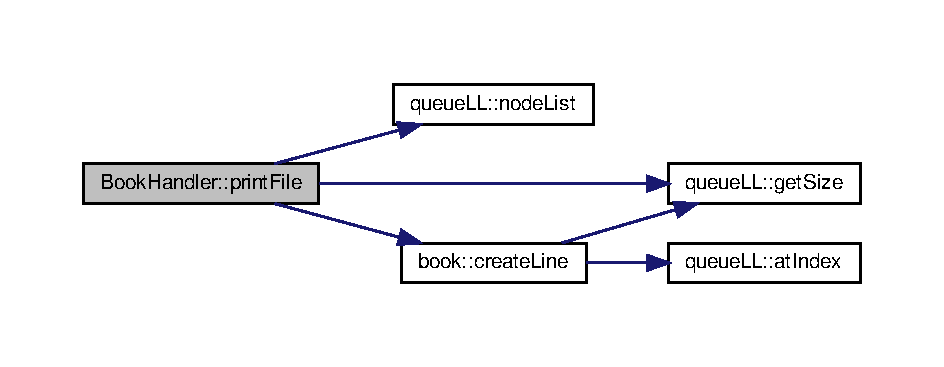
\includegraphics[width=350pt]{class_book_handler_a6794f0f693ff3048df64a5b254c183af_cgraph}
\end{center}
\end{figure}
Here is the caller graph for this function\+:
\nopagebreak
\begin{figure}[H]
\begin{center}
\leavevmode
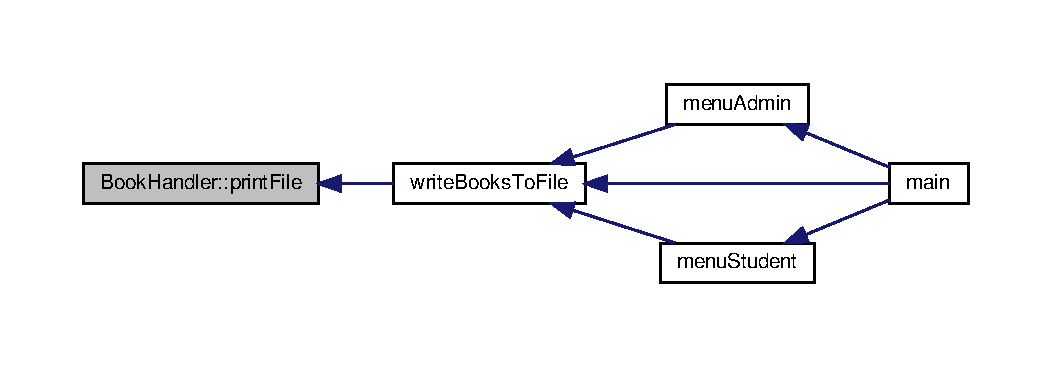
\includegraphics[width=350pt]{class_book_handler_a6794f0f693ff3048df64a5b254c183af_icgraph}
\end{center}
\end{figure}


\subsection{Member Data Documentation}
\mbox{\Hypertarget{class_book_handler_a13a6c78422b3ad7acd5ebdb9555a0286}\label{class_book_handler_a13a6c78422b3ad7acd5ebdb9555a0286}} 
\index{Book\+Handler@{Book\+Handler}!books\+List@{books\+List}}
\index{books\+List@{books\+List}!Book\+Handler@{Book\+Handler}}
\subsubsection{\texorpdfstring{books\+List}{booksList}}
{\footnotesize\ttfamily \hyperlink{classqueue_l_l}{queue\+LL}$<$\hyperlink{classbook}{book}$>$$\ast$ Book\+Handler\+::books\+List\hspace{0.3cm}{\ttfamily [private]}}

list of the books is kept in a queue 

Definition at line 76 of file Book\+Handler.\+h.



The documentation for this class was generated from the following files\+:\begin{DoxyCompactItemize}
\item 
src/\hyperlink{_book_handler_8h}{Book\+Handler.\+h}\item 
src/\hyperlink{_book_handler_8cpp}{Book\+Handler.\+cpp}\end{DoxyCompactItemize}

\hypertarget{class_node}{}\section{Node$<$ Type $>$ Class Template Reference}
\label{class_node}\index{Node$<$ Type $>$@{Node$<$ Type $>$}}


{\ttfamily \#include $<$Binary\+Tree.\+h$>$}



Collaboration diagram for Node$<$ Type $>$\+:
\nopagebreak
\begin{figure}[H]
\begin{center}
\leavevmode
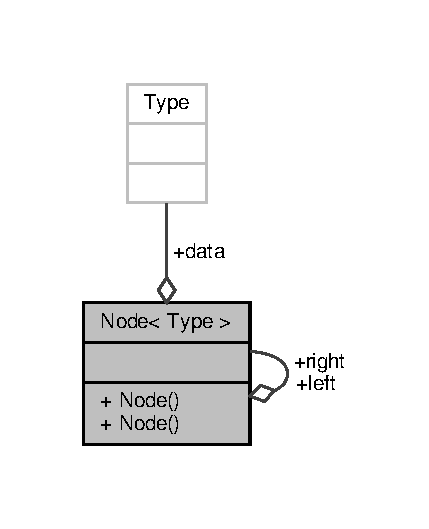
\includegraphics[width=206pt]{class_node__coll__graph}
\end{center}
\end{figure}
\subsection*{Public Member Functions}
\begin{DoxyCompactItemize}
\item 
\hyperlink{class_node_a238d6ebbae88f5a39daf8f31ff409164}{Node} (Type $\ast$\hyperlink{class_node_a8b322cc3cc17b752eb77533493713ddd}{data})
\item 
\hyperlink{class_node_ab27bbe294970f98f26b5d548dfbb50ca}{Node} ()
\end{DoxyCompactItemize}
\subsection*{Public Attributes}
\begin{DoxyCompactItemize}
\item 
Type $\ast$ \hyperlink{class_node_a8b322cc3cc17b752eb77533493713ddd}{data}
\item 
\hyperlink{class_node}{Node} $\ast$ \hyperlink{class_node_abb08a8b3137dd8fc8874348a439e01b4}{left}
\item 
\hyperlink{class_node}{Node} $\ast$ \hyperlink{class_node_a34452c0684d3cb1590406ad201b43e65}{right}
\end{DoxyCompactItemize}


\subsection{Detailed Description}
\subsubsection*{template$<$class Type$>$\newline
class Node$<$ Type $>$}

Generic class \hyperlink{class_node}{Node} is the node of the binary tree 
\begin{DoxyTemplParams}{Template Parameters}
{\em Type} & \\
\hline
\end{DoxyTemplParams}


Definition at line 18 of file Binary\+Tree.\+h.



\subsection{Constructor \& Destructor Documentation}
\mbox{\Hypertarget{class_node_a238d6ebbae88f5a39daf8f31ff409164}\label{class_node_a238d6ebbae88f5a39daf8f31ff409164}} 
\index{Node@{Node}!Node@{Node}}
\index{Node@{Node}!Node@{Node}}
\subsubsection{\texorpdfstring{Node()}{Node()}\hspace{0.1cm}{\footnotesize\ttfamily [1/2]}}
{\footnotesize\ttfamily template$<$class Type$>$ \\
\hyperlink{class_node}{Node}$<$ Type $>$\+::\hyperlink{class_node}{Node} (\begin{DoxyParamCaption}\item[{Type $\ast$}]{data }\end{DoxyParamCaption})\hspace{0.3cm}{\ttfamily [inline]}}

constructor function 
\begin{DoxyParams}{Parameters}
{\em data} & \\
\hline
\end{DoxyParams}


Definition at line 24 of file Binary\+Tree.\+h.


\begin{DoxyCode}
24                      \{
25         this->\hyperlink{class_node_a8b322cc3cc17b752eb77533493713ddd}{data} = \hyperlink{class_node_a8b322cc3cc17b752eb77533493713ddd}{data};
26         \hyperlink{class_node_abb08a8b3137dd8fc8874348a439e01b4}{left} = \hyperlink{class_node_a34452c0684d3cb1590406ad201b43e65}{right} = 0;
27     \}
\end{DoxyCode}
\mbox{\Hypertarget{class_node_ab27bbe294970f98f26b5d548dfbb50ca}\label{class_node_ab27bbe294970f98f26b5d548dfbb50ca}} 
\index{Node@{Node}!Node@{Node}}
\index{Node@{Node}!Node@{Node}}
\subsubsection{\texorpdfstring{Node()}{Node()}\hspace{0.1cm}{\footnotesize\ttfamily [2/2]}}
{\footnotesize\ttfamily template$<$class Type$>$ \\
\hyperlink{class_node}{Node}$<$ Type $>$\+::\hyperlink{class_node}{Node} (\begin{DoxyParamCaption}{ }\end{DoxyParamCaption})\hspace{0.3cm}{\ttfamily [inline]}}

constructor function 

Definition at line 31 of file Binary\+Tree.\+h.


\begin{DoxyCode}
31           \{
32         this->\hyperlink{class_node_a8b322cc3cc17b752eb77533493713ddd}{data} = 0;
33         \hyperlink{class_node_abb08a8b3137dd8fc8874348a439e01b4}{left} = \hyperlink{class_node_a34452c0684d3cb1590406ad201b43e65}{right} = 0;
34     \}
\end{DoxyCode}


\subsection{Member Data Documentation}
\mbox{\Hypertarget{class_node_a8b322cc3cc17b752eb77533493713ddd}\label{class_node_a8b322cc3cc17b752eb77533493713ddd}} 
\index{Node@{Node}!data@{data}}
\index{data@{data}!Node@{Node}}
\subsubsection{\texorpdfstring{data}{data}}
{\footnotesize\ttfamily template$<$class Type$>$ \\
Type$\ast$ \hyperlink{class_node}{Node}$<$ Type $>$\+::data}

data of \hyperlink{class_node}{Node} 

Definition at line 38 of file Binary\+Tree.\+h.

\mbox{\Hypertarget{class_node_abb08a8b3137dd8fc8874348a439e01b4}\label{class_node_abb08a8b3137dd8fc8874348a439e01b4}} 
\index{Node@{Node}!left@{left}}
\index{left@{left}!Node@{Node}}
\subsubsection{\texorpdfstring{left}{left}}
{\footnotesize\ttfamily template$<$class Type$>$ \\
\hyperlink{class_node}{Node}$\ast$ \hyperlink{class_node}{Node}$<$ Type $>$\+::left}

left pointer of \hyperlink{class_node}{Node} 

Definition at line 42 of file Binary\+Tree.\+h.

\mbox{\Hypertarget{class_node_a34452c0684d3cb1590406ad201b43e65}\label{class_node_a34452c0684d3cb1590406ad201b43e65}} 
\index{Node@{Node}!right@{right}}
\index{right@{right}!Node@{Node}}
\subsubsection{\texorpdfstring{right}{right}}
{\footnotesize\ttfamily template$<$class Type$>$ \\
\hyperlink{class_node}{Node}$\ast$ \hyperlink{class_node}{Node}$<$ Type $>$\+::right}

right pointer of \hyperlink{class_node}{Node} 

Definition at line 46 of file Binary\+Tree.\+h.



The documentation for this class was generated from the following file\+:\begin{DoxyCompactItemize}
\item 
src/\hyperlink{_binary_tree_8h}{Binary\+Tree.\+h}\end{DoxyCompactItemize}

\hypertarget{classqueue_l_l}{}\section{queue\+LL$<$ Type $>$ Class Template Reference}
\label{classqueue_l_l}\index{queue\+L\+L$<$ Type $>$@{queue\+L\+L$<$ Type $>$}}


{\ttfamily \#include $<$Queue\+L\+L.\+h$>$}



Collaboration diagram for queue\+LL$<$ Type $>$\+:
\nopagebreak
\begin{figure}[H]
\begin{center}
\leavevmode
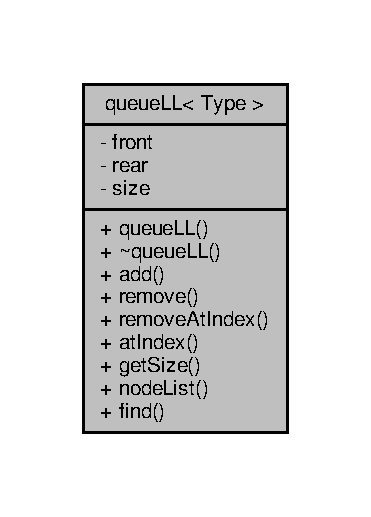
\includegraphics[width=178pt]{classqueue_l_l__coll__graph}
\end{center}
\end{figure}
\subsection*{Public Member Functions}
\begin{DoxyCompactItemize}
\item 
\hyperlink{classqueue_l_l_a8d7c7b45de1dcf799d5c7bad996094eb}{queue\+LL} ()
\item 
virtual \hyperlink{classqueue_l_l_af1560879b08f475cccfca106e0320cf6}{$\sim$queue\+LL} ()
\item 
void \hyperlink{classqueue_l_l_adcbcc26433da2c9d17b6cf0802d1d7d2}{add} (Type $\ast$value)
\item 
Type $\ast$ \hyperlink{classqueue_l_l_a4204a9db973b69be5824ca2495130b40}{remove} ()
\item 
Type $\ast$ \hyperlink{classqueue_l_l_abe3f175ee8c25c55d18650c5b13297b1}{remove\+At\+Index} (int index)
\item 
\hyperlink{classqueue_l_l_node}{queue\+L\+L\+Node}$<$ Type $>$ $\ast$ \hyperlink{classqueue_l_l_a6c8873be0f08b3b2e83a24469fbfaa5d}{at\+Index} (int index)
\item 
size\+\_\+t \hyperlink{classqueue_l_l_a8969feebcb563f0b489bc112422b9563}{get\+Size} () const
\item 
Type $\ast$$\ast$ \hyperlink{classqueue_l_l_ae9a479b9463f51c5148dd80b68335d32}{node\+List} ()
\item 
int \hyperlink{classqueue_l_l_af46d9d07b7528da834c2c37d752c29f5}{find} (Type data)
\end{DoxyCompactItemize}
\subsection*{Private Attributes}
\begin{DoxyCompactItemize}
\item 
\hyperlink{classqueue_l_l_node}{queue\+L\+L\+Node}$<$ Type $>$ $\ast$ \hyperlink{classqueue_l_l_a622ea439d113fe8e4616320ec2346d8b}{front}
\item 
\hyperlink{classqueue_l_l_node}{queue\+L\+L\+Node}$<$ Type $>$ $\ast$ \hyperlink{classqueue_l_l_aab0540567095f05fb1c981a2e7e4e93e}{rear}
\item 
size\+\_\+t \hyperlink{classqueue_l_l_af2ae538d6971624f1c8404d3a8502aa0}{size}
\end{DoxyCompactItemize}
\subsection*{Friends}
\begin{DoxyCompactItemize}
\item 
std\+::ostream \& \hyperlink{classqueue_l_l_a24d410ee760513f96b06f242b1025e8e}{operator$<$$<$} (std\+::ostream \&out, const \hyperlink{classqueue_l_l}{queue\+LL} \&b)
\end{DoxyCompactItemize}


\subsection{Detailed Description}
\subsubsection*{template$<$class Type$>$\newline
class queue\+L\+L$<$ Type $>$}

Generic class \hyperlink{classqueue_l_l}{queue\+LL} is the queue data structure which is implemented based on the linked list datastructure 
\begin{DoxyTemplParams}{Template Parameters}
{\em Type} & \\
\hline
\end{DoxyTemplParams}


Definition at line 52 of file Queue\+L\+L.\+h.



\subsection{Constructor \& Destructor Documentation}
\mbox{\Hypertarget{classqueue_l_l_a8d7c7b45de1dcf799d5c7bad996094eb}\label{classqueue_l_l_a8d7c7b45de1dcf799d5c7bad996094eb}} 
\index{queue\+LL@{queue\+LL}!queue\+LL@{queue\+LL}}
\index{queue\+LL@{queue\+LL}!queue\+LL@{queue\+LL}}
\subsubsection{\texorpdfstring{queue\+L\+L()}{queueLL()}}
{\footnotesize\ttfamily template$<$class Type$>$ \\
\hyperlink{classqueue_l_l}{queue\+LL}$<$ Type $>$\+::\hyperlink{classqueue_l_l}{queue\+LL} (\begin{DoxyParamCaption}{ }\end{DoxyParamCaption})\hspace{0.3cm}{\ttfamily [inline]}}

constructor function 

Definition at line 71 of file Queue\+L\+L.\+h.


\begin{DoxyCode}
71              \{
72         \hyperlink{classqueue_l_l_a622ea439d113fe8e4616320ec2346d8b}{front} = \hyperlink{classqueue_l_l_aab0540567095f05fb1c981a2e7e4e93e}{rear} = 0;
73         \hyperlink{classqueue_l_l_af2ae538d6971624f1c8404d3a8502aa0}{size} = 0;
74     \}
\end{DoxyCode}
\mbox{\Hypertarget{classqueue_l_l_af1560879b08f475cccfca106e0320cf6}\label{classqueue_l_l_af1560879b08f475cccfca106e0320cf6}} 
\index{queue\+LL@{queue\+LL}!````~queue\+LL@{$\sim$queue\+LL}}
\index{````~queue\+LL@{$\sim$queue\+LL}!queue\+LL@{queue\+LL}}
\subsubsection{\texorpdfstring{$\sim$queue\+L\+L()}{~queueLL()}}
{\footnotesize\ttfamily template$<$class Type$>$ \\
virtual \hyperlink{classqueue_l_l}{queue\+LL}$<$ Type $>$\+::$\sim$\hyperlink{classqueue_l_l}{queue\+LL} (\begin{DoxyParamCaption}{ }\end{DoxyParamCaption})\hspace{0.3cm}{\ttfamily [inline]}, {\ttfamily [virtual]}}

destructore function deletes the nodes in the queue and destroy the queuee 

Definition at line 79 of file Queue\+L\+L.\+h.


\begin{DoxyCode}
79                       \{
80         \hyperlink{classqueue_l_l_node}{queueLLNode<Type>} *temp;
81 
82         \textcolor{keywordflow}{while}(\hyperlink{classqueue_l_l_a622ea439d113fe8e4616320ec2346d8b}{front}!=0)
83         \{
84             temp=\hyperlink{classqueue_l_l_a622ea439d113fe8e4616320ec2346d8b}{front};
85             \hyperlink{classqueue_l_l_a622ea439d113fe8e4616320ec2346d8b}{front}=\hyperlink{classqueue_l_l_a622ea439d113fe8e4616320ec2346d8b}{front}->next;
86             \textcolor{keyword}{delete} temp;
87             \hyperlink{classqueue_l_l_af2ae538d6971624f1c8404d3a8502aa0}{size}--;
88         \}
89         \hyperlink{classqueue_l_l_aab0540567095f05fb1c981a2e7e4e93e}{rear}=0;
90         \hyperlink{classqueue_l_l_af2ae538d6971624f1c8404d3a8502aa0}{size}=0;
91     \}
\end{DoxyCode}


\subsection{Member Function Documentation}
\mbox{\Hypertarget{classqueue_l_l_adcbcc26433da2c9d17b6cf0802d1d7d2}\label{classqueue_l_l_adcbcc26433da2c9d17b6cf0802d1d7d2}} 
\index{queue\+LL@{queue\+LL}!add@{add}}
\index{add@{add}!queue\+LL@{queue\+LL}}
\subsubsection{\texorpdfstring{add()}{add()}}
{\footnotesize\ttfamily template$<$class Type$>$ \\
void \hyperlink{classqueue_l_l}{queue\+LL}$<$ Type $>$\+::add (\begin{DoxyParamCaption}\item[{Type $\ast$}]{value }\end{DoxyParamCaption})\hspace{0.3cm}{\ttfamily [inline]}}

function adds a new node to rear of the queue 
\begin{DoxyParams}{Parameters}
{\em value} & data of the node \\
\hline
\end{DoxyParams}


Definition at line 96 of file Queue\+L\+L.\+h.


\begin{DoxyCode}
96                            \{
97 
98         \textcolor{comment}{// Create a new LL node}
99         \hyperlink{classqueue_l_l_node}{queueLLNode<Type>}* temp = \textcolor{keyword}{new} \hyperlink{classqueue_l_l_node}{queueLLNode<Type>}(value);
100 
101         \textcolor{keywordflow}{if} (\hyperlink{classqueue_l_l_aab0540567095f05fb1c981a2e7e4e93e}{rear} == 0) \{    \textcolor{comment}{// If queue is empty,}
102             \hyperlink{classqueue_l_l_a622ea439d113fe8e4616320ec2346d8b}{front} = \hyperlink{classqueue_l_l_aab0540567095f05fb1c981a2e7e4e93e}{rear} = temp;
103             \hyperlink{classqueue_l_l_af2ae538d6971624f1c8404d3a8502aa0}{size}++;
104         \}
105         \textcolor{keywordflow}{else}\{   \textcolor{comment}{// Add the new node at the end of queue}
106             \hyperlink{classqueue_l_l_aab0540567095f05fb1c981a2e7e4e93e}{rear}->next = temp;
107             \hyperlink{classqueue_l_l_aab0540567095f05fb1c981a2e7e4e93e}{rear} = temp;
108             \hyperlink{classqueue_l_l_af2ae538d6971624f1c8404d3a8502aa0}{size}++;
109         \}
110     \}
\end{DoxyCode}
Here is the caller graph for this function\+:
\nopagebreak
\begin{figure}[H]
\begin{center}
\leavevmode
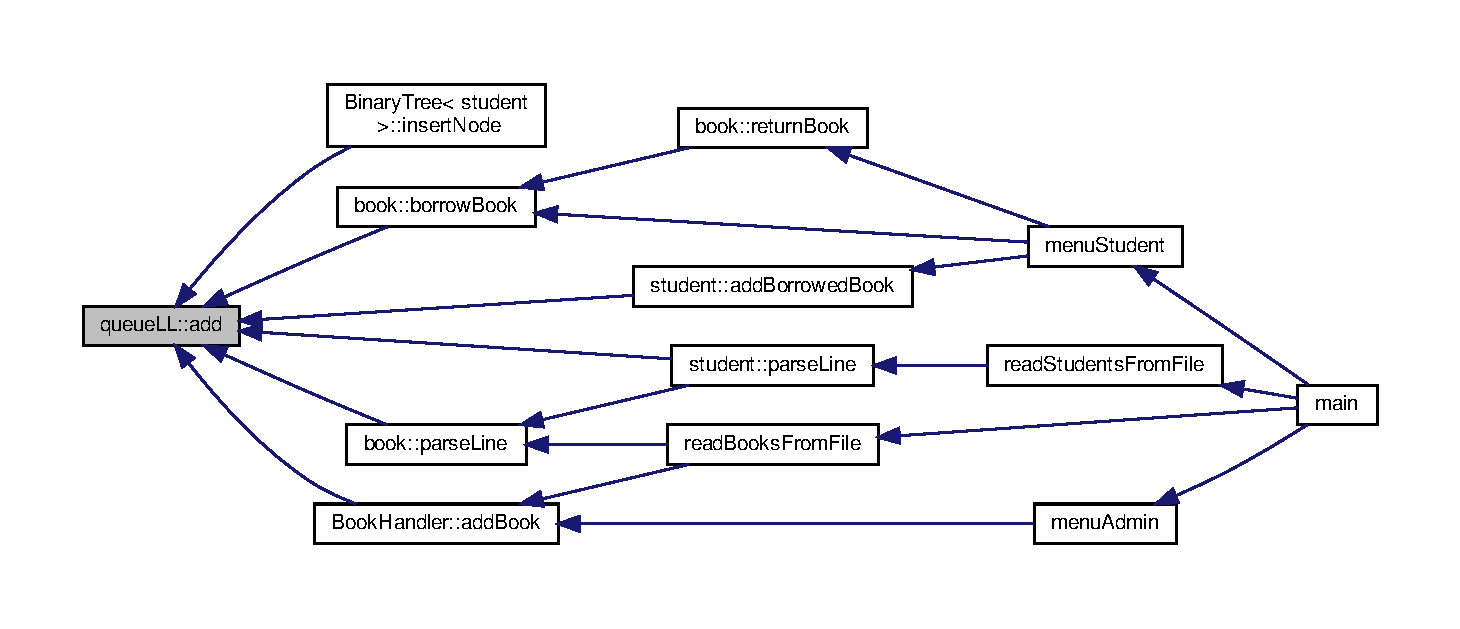
\includegraphics[width=350pt]{classqueue_l_l_adcbcc26433da2c9d17b6cf0802d1d7d2_icgraph}
\end{center}
\end{figure}
\mbox{\Hypertarget{classqueue_l_l_a6c8873be0f08b3b2e83a24469fbfaa5d}\label{classqueue_l_l_a6c8873be0f08b3b2e83a24469fbfaa5d}} 
\index{queue\+LL@{queue\+LL}!at\+Index@{at\+Index}}
\index{at\+Index@{at\+Index}!queue\+LL@{queue\+LL}}
\subsubsection{\texorpdfstring{at\+Index()}{atIndex()}}
{\footnotesize\ttfamily template$<$class Type$>$ \\
\hyperlink{classqueue_l_l_node}{queue\+L\+L\+Node}$<$Type$>$$\ast$ \hyperlink{classqueue_l_l}{queue\+LL}$<$ Type $>$\+::at\+Index (\begin{DoxyParamCaption}\item[{int}]{index }\end{DoxyParamCaption})\hspace{0.3cm}{\ttfamily [inline]}}

function returns the node at location index of the queue \begin{DoxyReturn}{Returns}
pointer to the node which is located at location index of the queue 
\end{DoxyReturn}


Definition at line 172 of file Queue\+L\+L.\+h.


\begin{DoxyCode}
173     \{
174 
175         \hyperlink{classqueue_l_l_node}{queueLLNode<Type>}* temp = \hyperlink{classqueue_l_l_a622ea439d113fe8e4616320ec2346d8b}{front};
176 
177 
178         \textcolor{keywordtype}{int} count = 0;
179         \textcolor{keywordflow}{while} (temp != 0)
180         \{
181             \textcolor{keywordflow}{if} (count == index)
182                 \textcolor{keywordflow}{return}(temp);
183             count++;
184             temp = temp->\hyperlink{classqueue_l_l_node_ab8367d61c51828d9f21d72537b62735f}{next};
185         \}
186         std::cout<<\textcolor{stringliteral}{"Node at index:"}<<index<<\textcolor{stringliteral}{" does not exist\(\backslash\)n"};
187 
188         \textcolor{keywordflow}{return} 0;
189     \}
\end{DoxyCode}
Here is the caller graph for this function\+:
\nopagebreak
\begin{figure}[H]
\begin{center}
\leavevmode
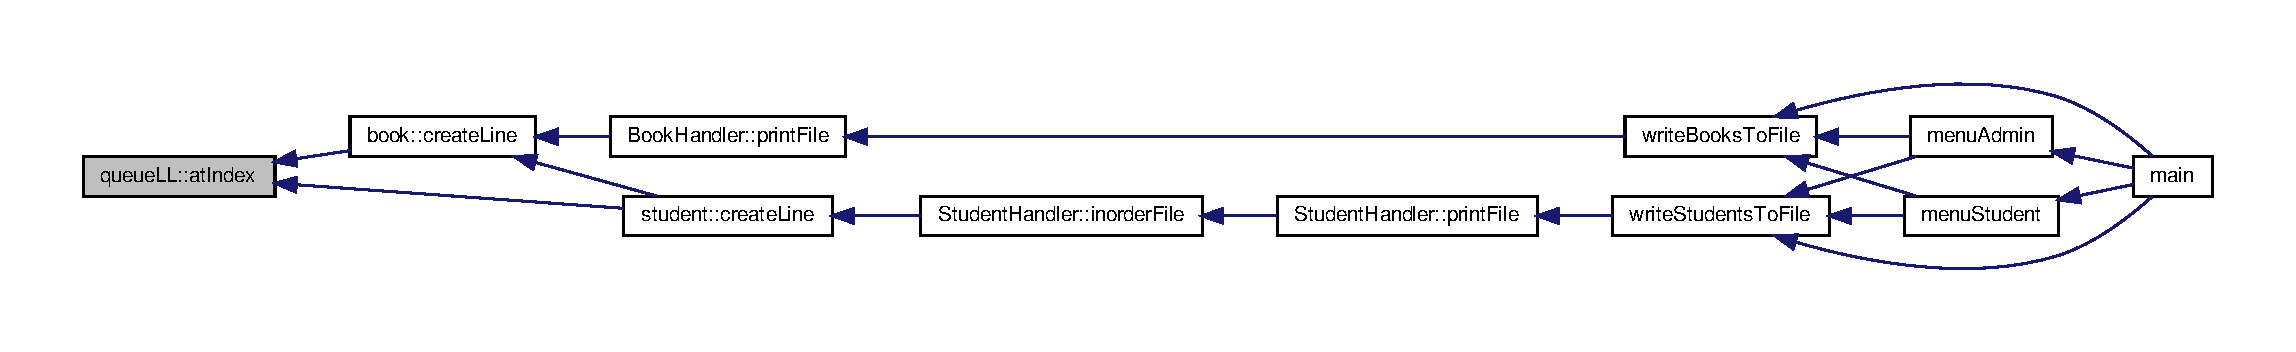
\includegraphics[width=350pt]{classqueue_l_l_a6c8873be0f08b3b2e83a24469fbfaa5d_icgraph}
\end{center}
\end{figure}
\mbox{\Hypertarget{classqueue_l_l_af46d9d07b7528da834c2c37d752c29f5}\label{classqueue_l_l_af46d9d07b7528da834c2c37d752c29f5}} 
\index{queue\+LL@{queue\+LL}!find@{find}}
\index{find@{find}!queue\+LL@{queue\+LL}}
\subsubsection{\texorpdfstring{find()}{find()}}
{\footnotesize\ttfamily template$<$class Type$>$ \\
int \hyperlink{classqueue_l_l}{queue\+LL}$<$ Type $>$\+::find (\begin{DoxyParamCaption}\item[{Type}]{data }\end{DoxyParamCaption})\hspace{0.3cm}{\ttfamily [inline]}}

functions finds the index of the node with specififc data 
\begin{DoxyParams}{Parameters}
{\em data} & data of the node \\
\hline
\end{DoxyParams}
\begin{DoxyReturn}{Returns}
\+: index of the node 
\end{DoxyReturn}


Definition at line 240 of file Queue\+L\+L.\+h.


\begin{DoxyCode}
240                        \{
241         \textcolor{keywordtype}{int} i=-1;
242         \textcolor{keywordflow}{if}(\hyperlink{classqueue_l_l_a622ea439d113fe8e4616320ec2346d8b}{front})\{
243             i=0;
244             \hyperlink{classqueue_l_l_node}{queueLLNode<Type>} *temp=\hyperlink{classqueue_l_l_a622ea439d113fe8e4616320ec2346d8b}{front};
245             \textcolor{keywordflow}{while}(temp && *(temp->\hyperlink{classqueue_l_l_node_a20b1170d8c5852b7dc01e56fda4e4206}{data})!=data)\{
246                 temp = temp->\hyperlink{classqueue_l_l_node_ab8367d61c51828d9f21d72537b62735f}{next};
247                 i++;
248             \}
249             \textcolor{keywordflow}{if}(temp==NULL)\{
250                 i = -1;
251             \}
252             \textcolor{keywordflow}{else} \textcolor{keywordflow}{if}(*temp->\hyperlink{classqueue_l_l_node_a20b1170d8c5852b7dc01e56fda4e4206}{data}!=data)\{
253                 i = -1;
254             \}
255         \}
256         \textcolor{keywordflow}{return} i;
257     \}
\end{DoxyCode}
Here is the caller graph for this function\+:
\nopagebreak
\begin{figure}[H]
\begin{center}
\leavevmode
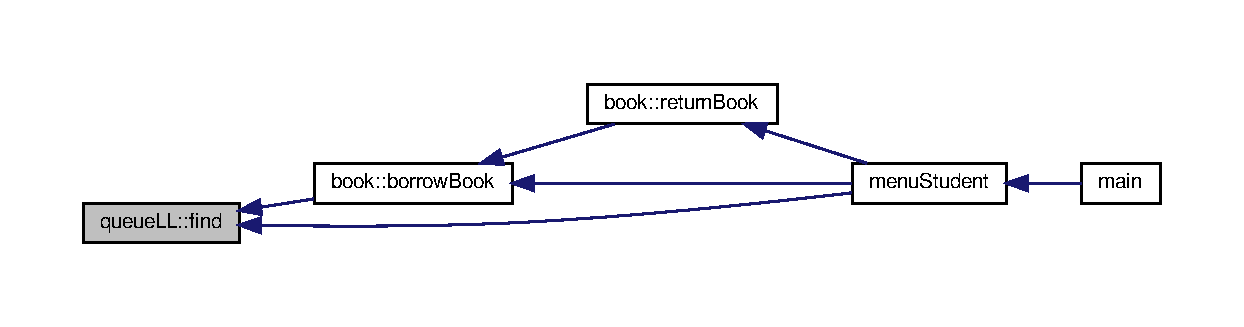
\includegraphics[width=350pt]{classqueue_l_l_af46d9d07b7528da834c2c37d752c29f5_icgraph}
\end{center}
\end{figure}
\mbox{\Hypertarget{classqueue_l_l_a8969feebcb563f0b489bc112422b9563}\label{classqueue_l_l_a8969feebcb563f0b489bc112422b9563}} 
\index{queue\+LL@{queue\+LL}!get\+Size@{get\+Size}}
\index{get\+Size@{get\+Size}!queue\+LL@{queue\+LL}}
\subsubsection{\texorpdfstring{get\+Size()}{getSize()}}
{\footnotesize\ttfamily template$<$class Type$>$ \\
size\+\_\+t \hyperlink{classqueue_l_l}{queue\+LL}$<$ Type $>$\+::get\+Size (\begin{DoxyParamCaption}{ }\end{DoxyParamCaption}) const\hspace{0.3cm}{\ttfamily [inline]}}

function return size of the queue \begin{DoxyReturn}{Returns}
size of the queue 
\end{DoxyReturn}


Definition at line 218 of file Queue\+L\+L.\+h.


\begin{DoxyCode}
218                            \{
219         \textcolor{keywordflow}{return} \hyperlink{classqueue_l_l_af2ae538d6971624f1c8404d3a8502aa0}{size};
220     \}
\end{DoxyCode}
Here is the caller graph for this function\+:
\nopagebreak
\begin{figure}[H]
\begin{center}
\leavevmode
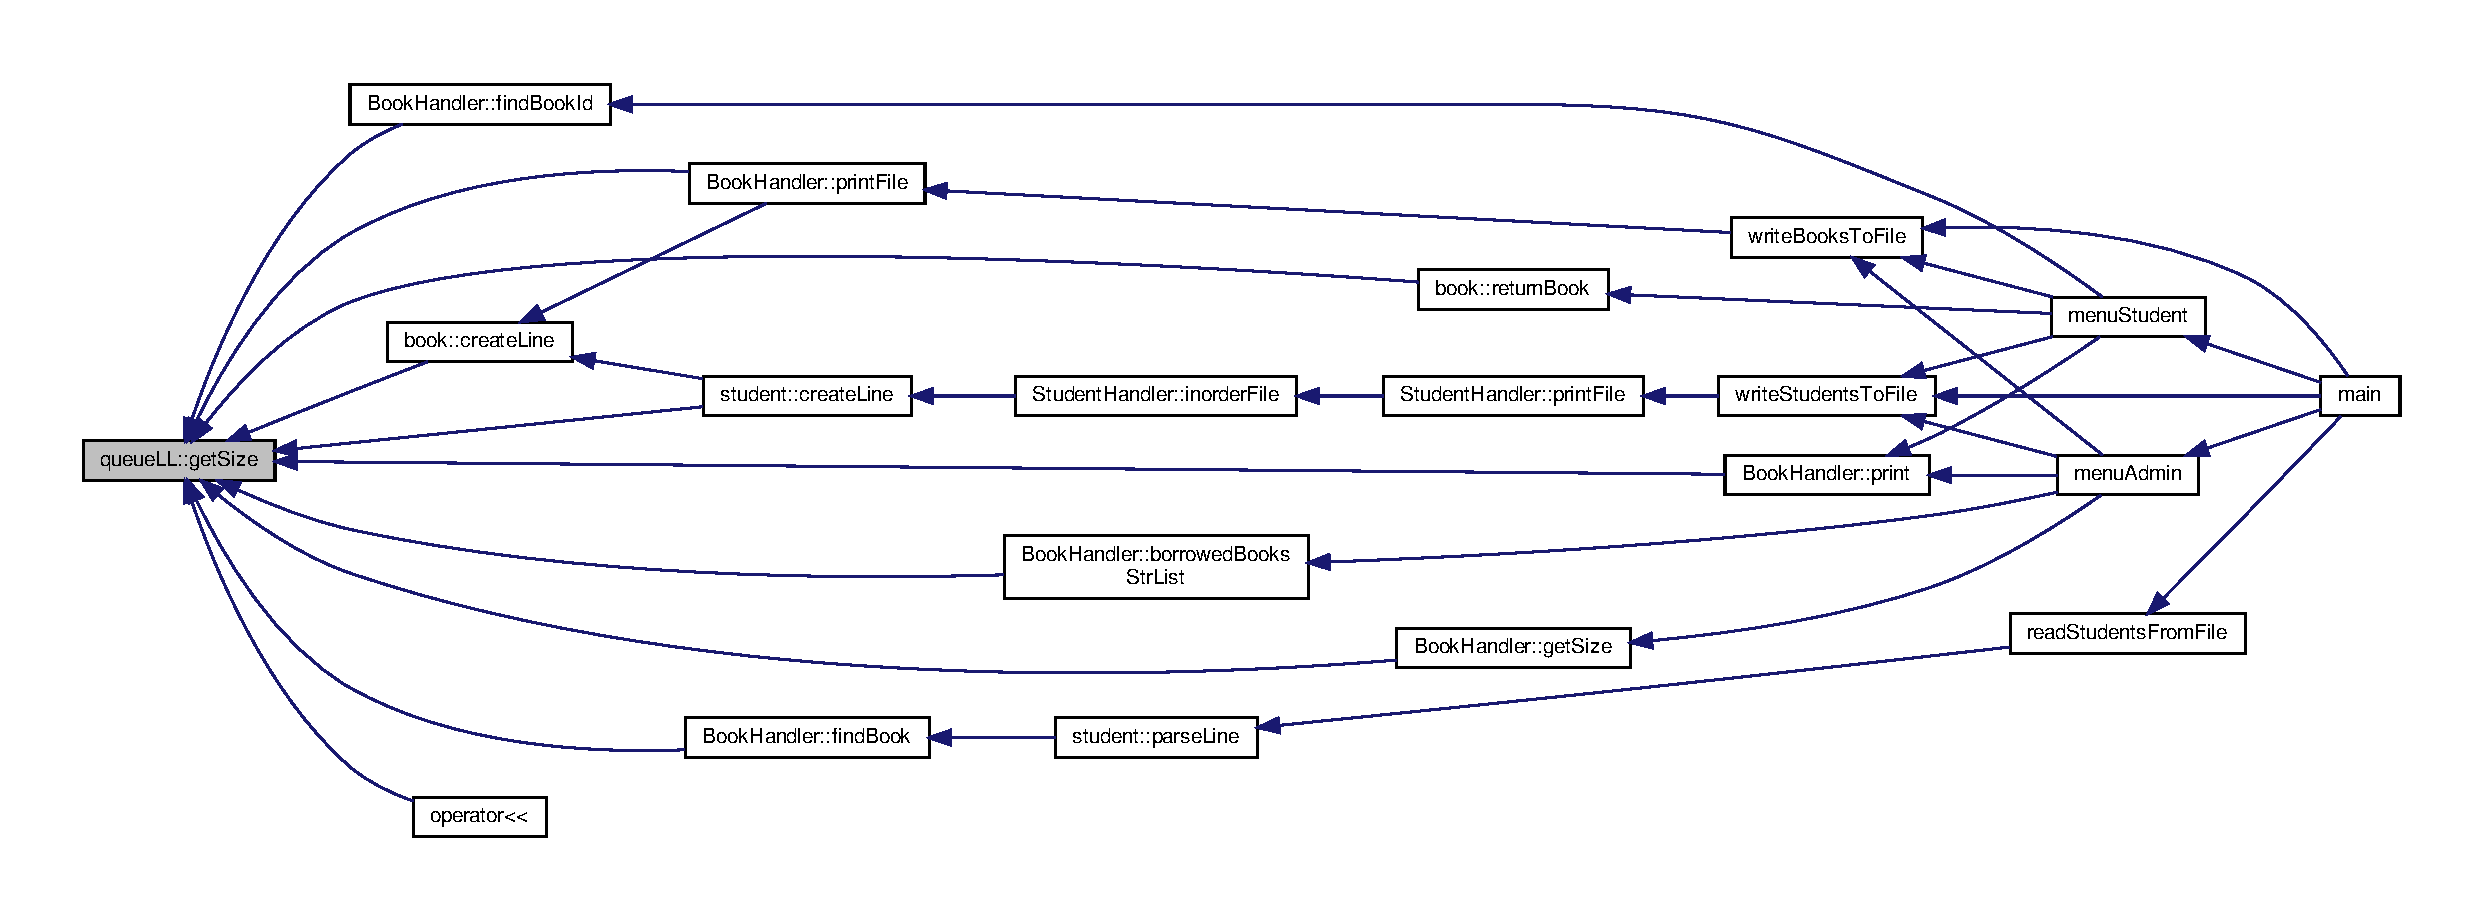
\includegraphics[width=350pt]{classqueue_l_l_a8969feebcb563f0b489bc112422b9563_icgraph}
\end{center}
\end{figure}
\mbox{\Hypertarget{classqueue_l_l_ae9a479b9463f51c5148dd80b68335d32}\label{classqueue_l_l_ae9a479b9463f51c5148dd80b68335d32}} 
\index{queue\+LL@{queue\+LL}!node\+List@{node\+List}}
\index{node\+List@{node\+List}!queue\+LL@{queue\+LL}}
\subsubsection{\texorpdfstring{node\+List()}{nodeList()}}
{\footnotesize\ttfamily template$<$class Type$>$ \\
Type$\ast$$\ast$ \hyperlink{classqueue_l_l}{queue\+LL}$<$ Type $>$\+::node\+List (\begin{DoxyParamCaption}{ }\end{DoxyParamCaption})\hspace{0.3cm}{\ttfamily [inline]}}

function returns list of the nodes \begin{DoxyReturn}{Returns}
list of the nodes 
\end{DoxyReturn}


Definition at line 225 of file Queue\+L\+L.\+h.


\begin{DoxyCode}
225                      \{
226         Type ** list = \textcolor{keyword}{new}  Type*[\hyperlink{classqueue_l_l_af2ae538d6971624f1c8404d3a8502aa0}{size}];
227         \textcolor{keywordtype}{int} i=0;
228         \hyperlink{classqueue_l_l_node}{queueLLNode<Type>} *temp=\hyperlink{classqueue_l_l_a622ea439d113fe8e4616320ec2346d8b}{front};
229         \textcolor{keywordflow}{while}(temp)\{
230             list[i++] = temp->\hyperlink{classqueue_l_l_node_a20b1170d8c5852b7dc01e56fda4e4206}{data} ;
231             temp = temp->\hyperlink{classqueue_l_l_node_ab8367d61c51828d9f21d72537b62735f}{next};
232         \}
233         \textcolor{keywordflow}{return} list;
234     \}
\end{DoxyCode}
Here is the caller graph for this function\+:
\nopagebreak
\begin{figure}[H]
\begin{center}
\leavevmode
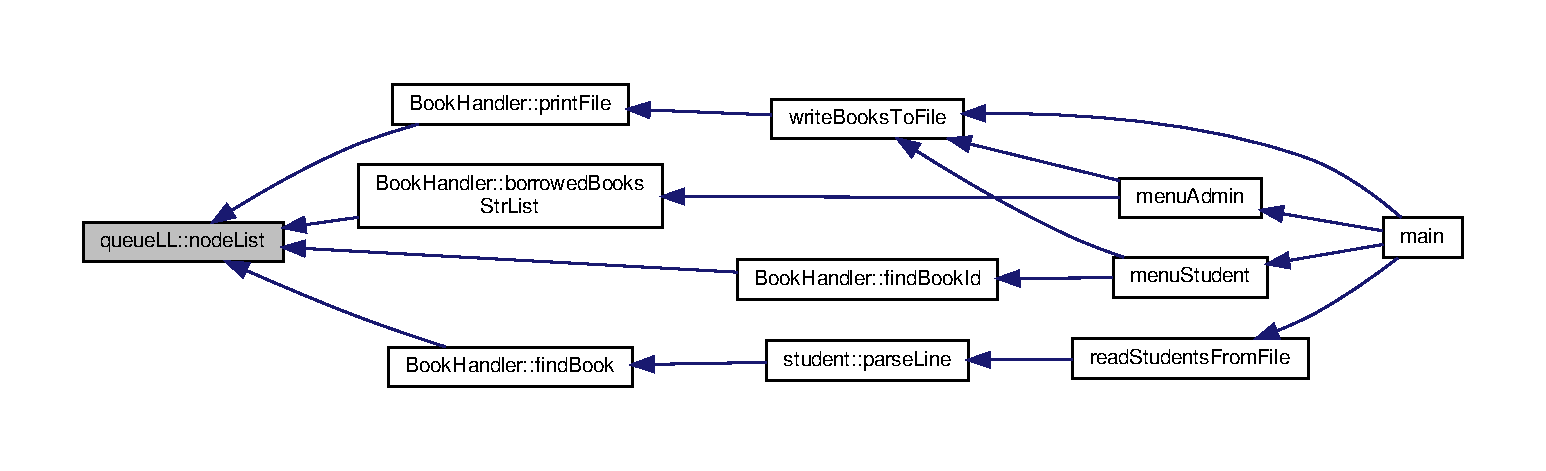
\includegraphics[width=350pt]{classqueue_l_l_ae9a479b9463f51c5148dd80b68335d32_icgraph}
\end{center}
\end{figure}
\mbox{\Hypertarget{classqueue_l_l_a4204a9db973b69be5824ca2495130b40}\label{classqueue_l_l_a4204a9db973b69be5824ca2495130b40}} 
\index{queue\+LL@{queue\+LL}!remove@{remove}}
\index{remove@{remove}!queue\+LL@{queue\+LL}}
\subsubsection{\texorpdfstring{remove()}{remove()}}
{\footnotesize\ttfamily template$<$class Type$>$ \\
Type$\ast$ \hyperlink{classqueue_l_l}{queue\+LL}$<$ Type $>$\+::remove (\begin{DoxyParamCaption}{ }\end{DoxyParamCaption})\hspace{0.3cm}{\ttfamily [inline]}}

function removes and returns the data of the first node of the queue \begin{DoxyReturn}{Returns}
pointer to the data of the first node of the queue 
\end{DoxyReturn}


Definition at line 115 of file Queue\+L\+L.\+h.


\begin{DoxyCode}
115                     \{
116         Type * returnNode = 0;
117         \textcolor{comment}{// If queue is empty, return false.}
118         \textcolor{keywordflow}{if} (\hyperlink{classqueue_l_l_a622ea439d113fe8e4616320ec2346d8b}{front} == 0) \{
119             std::cout<<\textcolor{stringliteral}{"Queue is empty."};
120         \}
121         \textcolor{keywordflow}{else}\{
122             \hyperlink{classqueue_l_l_node}{queueLLNode<Type>}* temp = \hyperlink{classqueue_l_l_a622ea439d113fe8e4616320ec2346d8b}{front};
123             \hyperlink{classqueue_l_l_a622ea439d113fe8e4616320ec2346d8b}{front} = \hyperlink{classqueue_l_l_a622ea439d113fe8e4616320ec2346d8b}{front}->next;
124             \textcolor{comment}{//queue gets empty}
125             \textcolor{keywordflow}{if} (\hyperlink{classqueue_l_l_a622ea439d113fe8e4616320ec2346d8b}{front} == 0)
126                 \hyperlink{classqueue_l_l_aab0540567095f05fb1c981a2e7e4e93e}{rear} = 0;
127             returnNode = temp->\hyperlink{classqueue_l_l_node_a20b1170d8c5852b7dc01e56fda4e4206}{data};
128             \hyperlink{classqueue_l_l_af2ae538d6971624f1c8404d3a8502aa0}{size}--;
129             \textcolor{keyword}{delete} (temp);
130             temp = 0;
131         \}
132         \textcolor{keywordflow}{return} returnNode;
133     \}
\end{DoxyCode}
Here is the caller graph for this function\+:
\nopagebreak
\begin{figure}[H]
\begin{center}
\leavevmode
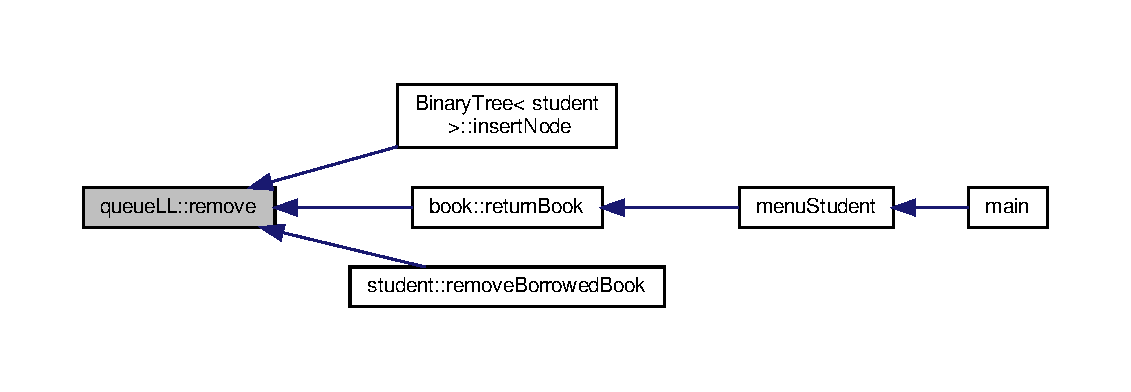
\includegraphics[width=350pt]{classqueue_l_l_a4204a9db973b69be5824ca2495130b40_icgraph}
\end{center}
\end{figure}
\mbox{\Hypertarget{classqueue_l_l_abe3f175ee8c25c55d18650c5b13297b1}\label{classqueue_l_l_abe3f175ee8c25c55d18650c5b13297b1}} 
\index{queue\+LL@{queue\+LL}!remove\+At\+Index@{remove\+At\+Index}}
\index{remove\+At\+Index@{remove\+At\+Index}!queue\+LL@{queue\+LL}}
\subsubsection{\texorpdfstring{remove\+At\+Index()}{removeAtIndex()}}
{\footnotesize\ttfamily template$<$class Type$>$ \\
Type$\ast$ \hyperlink{classqueue_l_l}{queue\+LL}$<$ Type $>$\+::remove\+At\+Index (\begin{DoxyParamCaption}\item[{int}]{index }\end{DoxyParamCaption})\hspace{0.3cm}{\ttfamily [inline]}}

function removes and returns the data of the node at location index of the queue \begin{DoxyReturn}{Returns}
pointer to the data of the node which is located at location index of the queue 
\end{DoxyReturn}


Definition at line 138 of file Queue\+L\+L.\+h.


\begin{DoxyCode}
139     \{
140         Type * returnNode = 0;
141         \hyperlink{classqueue_l_l_node}{queueLLNode<Type>}* temp = \hyperlink{classqueue_l_l_a622ea439d113fe8e4616320ec2346d8b}{front};
142         \hyperlink{classqueue_l_l_node}{queueLLNode<Type>}* prev = \hyperlink{classqueue_l_l_a622ea439d113fe8e4616320ec2346d8b}{front};
143 
144 
145         \textcolor{keywordtype}{int} count = 0;
146         \textcolor{keywordflow}{while} (temp != 0)
147         \{
148             \textcolor{keywordflow}{if} (count == index)\{
149                 \textcolor{keywordflow}{if}(temp!=\hyperlink{classqueue_l_l_a622ea439d113fe8e4616320ec2346d8b}{front})
150                     prev->\hyperlink{classqueue_l_l_node_ab8367d61c51828d9f21d72537b62735f}{next} = temp->\hyperlink{classqueue_l_l_node_ab8367d61c51828d9f21d72537b62735f}{next};
151                 \textcolor{keywordflow}{else}\{
152                     \hyperlink{classqueue_l_l_a622ea439d113fe8e4616320ec2346d8b}{front}=\hyperlink{classqueue_l_l_aab0540567095f05fb1c981a2e7e4e93e}{rear} = 0;
153                 \}
154                 returnNode = temp->\hyperlink{classqueue_l_l_node_a20b1170d8c5852b7dc01e56fda4e4206}{data};
155                 \hyperlink{classqueue_l_l_af2ae538d6971624f1c8404d3a8502aa0}{size}--;
156                 \textcolor{keyword}{delete} (temp);
157                 temp = 0;
158                 \textcolor{keywordflow}{return} returnNode;
159             \}
160             count++;
161             prev=temp;
162             temp = temp->\hyperlink{classqueue_l_l_node_ab8367d61c51828d9f21d72537b62735f}{next};
163         \}
164         std::cout<<\textcolor{stringliteral}{"Node at index:"}<<index<<\textcolor{stringliteral}{" does not exist\(\backslash\)n"};
165 
166         \textcolor{keywordflow}{return} 0;
167     \}
\end{DoxyCode}
Here is the caller graph for this function\+:
\nopagebreak
\begin{figure}[H]
\begin{center}
\leavevmode
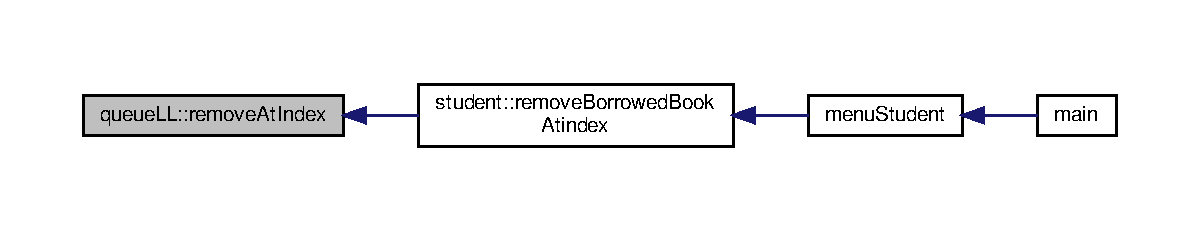
\includegraphics[width=350pt]{classqueue_l_l_abe3f175ee8c25c55d18650c5b13297b1_icgraph}
\end{center}
\end{figure}


\subsection{Friends And Related Function Documentation}
\mbox{\Hypertarget{classqueue_l_l_a24d410ee760513f96b06f242b1025e8e}\label{classqueue_l_l_a24d410ee760513f96b06f242b1025e8e}} 
\index{queue\+LL@{queue\+LL}!operator$<$$<$@{operator$<$$<$}}
\index{operator$<$$<$@{operator$<$$<$}!queue\+LL@{queue\+LL}}
\subsubsection{\texorpdfstring{operator$<$$<$}{operator<<}}
{\footnotesize\ttfamily template$<$class Type$>$ \\
std\+::ostream\& operator$<$$<$ (\begin{DoxyParamCaption}\item[{std\+::ostream \&}]{out,  }\item[{const \hyperlink{classqueue_l_l}{queue\+LL}$<$ Type $>$ \&}]{b }\end{DoxyParamCaption})\hspace{0.3cm}{\ttfamily [friend]}}

function overloads operator $<$$<$ 
\begin{DoxyParams}{Parameters}
{\em out} & output stream \\
\hline
{\em b} & queue object \\
\hline
\end{DoxyParams}
\begin{DoxyReturn}{Returns}

\end{DoxyReturn}


Definition at line 196 of file Queue\+L\+L.\+h.


\begin{DoxyCode}
196                                                                       \{
197 
198         \textcolor{keywordflow}{if}(b.\hyperlink{classqueue_l_l_a622ea439d113fe8e4616320ec2346d8b}{front}==0)\{
199             out<<\textcolor{stringliteral}{"Queue is empty."};
200         \}
201         \textcolor{keywordflow}{else}\{
202             \hyperlink{classqueue_l_l_node}{queueLLNode<Type>} *temp=b.\hyperlink{classqueue_l_l_a622ea439d113fe8e4616320ec2346d8b}{front};
203             \textcolor{keywordflow}{while}(temp)\{
204                 out<< *temp->\hyperlink{classqueue_l_l_node_a20b1170d8c5852b7dc01e56fda4e4206}{data} <<\textcolor{stringliteral}{" \(\backslash\)n"};
205                 temp = temp->\hyperlink{classqueue_l_l_node_ab8367d61c51828d9f21d72537b62735f}{next};
206             \}
207         \}
208 \textcolor{comment}{//      os<<std::endl;}
209         \textcolor{keywordflow}{return} out;
210     \}
\end{DoxyCode}


\subsection{Member Data Documentation}
\mbox{\Hypertarget{classqueue_l_l_a622ea439d113fe8e4616320ec2346d8b}\label{classqueue_l_l_a622ea439d113fe8e4616320ec2346d8b}} 
\index{queue\+LL@{queue\+LL}!front@{front}}
\index{front@{front}!queue\+LL@{queue\+LL}}
\subsubsection{\texorpdfstring{front}{front}}
{\footnotesize\ttfamily template$<$class Type$>$ \\
\hyperlink{classqueue_l_l_node}{queue\+L\+L\+Node}$<$Type$>$$\ast$ \hyperlink{classqueue_l_l}{queue\+LL}$<$ Type $>$\+::front\hspace{0.3cm}{\ttfamily [private]}}

pointer to the first node of the queue 

Definition at line 57 of file Queue\+L\+L.\+h.

\mbox{\Hypertarget{classqueue_l_l_aab0540567095f05fb1c981a2e7e4e93e}\label{classqueue_l_l_aab0540567095f05fb1c981a2e7e4e93e}} 
\index{queue\+LL@{queue\+LL}!rear@{rear}}
\index{rear@{rear}!queue\+LL@{queue\+LL}}
\subsubsection{\texorpdfstring{rear}{rear}}
{\footnotesize\ttfamily template$<$class Type$>$ \\
\hyperlink{classqueue_l_l_node}{queue\+L\+L\+Node}$<$Type$>$$\ast$ \hyperlink{classqueue_l_l}{queue\+LL}$<$ Type $>$\+::rear\hspace{0.3cm}{\ttfamily [private]}}

pointer to the last node of the queue 

Definition at line 61 of file Queue\+L\+L.\+h.

\mbox{\Hypertarget{classqueue_l_l_af2ae538d6971624f1c8404d3a8502aa0}\label{classqueue_l_l_af2ae538d6971624f1c8404d3a8502aa0}} 
\index{queue\+LL@{queue\+LL}!size@{size}}
\index{size@{size}!queue\+LL@{queue\+LL}}
\subsubsection{\texorpdfstring{size}{size}}
{\footnotesize\ttfamily template$<$class Type$>$ \\
size\+\_\+t \hyperlink{classqueue_l_l}{queue\+LL}$<$ Type $>$\+::size\hspace{0.3cm}{\ttfamily [private]}}

size of the queue 

Definition at line 65 of file Queue\+L\+L.\+h.



The documentation for this class was generated from the following file\+:\begin{DoxyCompactItemize}
\item 
src/\hyperlink{_queue_l_l_8h}{Queue\+L\+L.\+h}\end{DoxyCompactItemize}

\hypertarget{classqueue_l_l_node}{}\section{queue\+L\+L\+Node$<$ Type $>$ Class Template Reference}
\label{classqueue_l_l_node}\index{queue\+L\+L\+Node$<$ Type $>$@{queue\+L\+L\+Node$<$ Type $>$}}


{\ttfamily \#include $<$Queue\+L\+L.\+h$>$}



Collaboration diagram for queue\+L\+L\+Node$<$ Type $>$\+:
\nopagebreak
\begin{figure}[H]
\begin{center}
\leavevmode
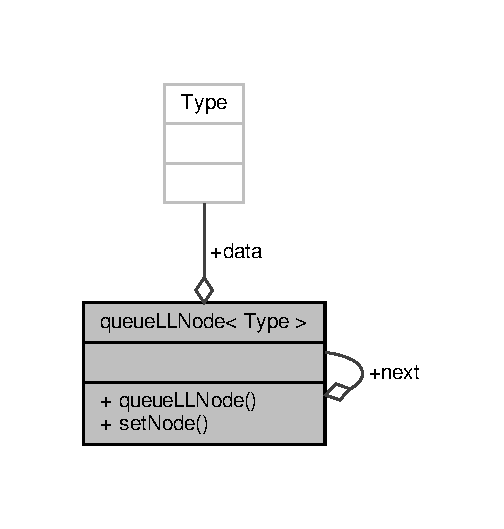
\includegraphics[width=242pt]{classqueue_l_l_node__coll__graph}
\end{center}
\end{figure}
\subsection*{Public Member Functions}
\begin{DoxyCompactItemize}
\item 
\hyperlink{classqueue_l_l_node_a52a32e9e79f0b6cedeec1b9e68589354}{queue\+L\+L\+Node} (Type $\ast$\hyperlink{classqueue_l_l_node_a20b1170d8c5852b7dc01e56fda4e4206}{data})
\item 
void \hyperlink{classqueue_l_l_node_ac264831406ec126a6ece6b5522d89dcd}{set\+Node} (Type $\ast$\hyperlink{classqueue_l_l_node_a20b1170d8c5852b7dc01e56fda4e4206}{data}, \hyperlink{classqueue_l_l_node}{queue\+L\+L\+Node} $\ast$\hyperlink{classqueue_l_l_node_ab8367d61c51828d9f21d72537b62735f}{next})
\end{DoxyCompactItemize}
\subsection*{Public Attributes}
\begin{DoxyCompactItemize}
\item 
Type $\ast$ \hyperlink{classqueue_l_l_node_a20b1170d8c5852b7dc01e56fda4e4206}{data}
\item 
\hyperlink{classqueue_l_l_node}{queue\+L\+L\+Node} $\ast$ \hyperlink{classqueue_l_l_node_ab8367d61c51828d9f21d72537b62735f}{next}
\end{DoxyCompactItemize}


\subsection{Detailed Description}
\subsubsection*{template$<$class Type$>$\newline
class queue\+L\+L\+Node$<$ Type $>$}

Generic class \hyperlink{classqueue_l_l_node}{queue\+L\+L\+Node} is the node of the queue class 
\begin{DoxyTemplParams}{Template Parameters}
{\em Type} & \\
\hline
\end{DoxyTemplParams}


Definition at line 18 of file Queue\+L\+L.\+h.



\subsection{Constructor \& Destructor Documentation}
\mbox{\Hypertarget{classqueue_l_l_node_a52a32e9e79f0b6cedeec1b9e68589354}\label{classqueue_l_l_node_a52a32e9e79f0b6cedeec1b9e68589354}} 
\index{queue\+L\+L\+Node@{queue\+L\+L\+Node}!queue\+L\+L\+Node@{queue\+L\+L\+Node}}
\index{queue\+L\+L\+Node@{queue\+L\+L\+Node}!queue\+L\+L\+Node@{queue\+L\+L\+Node}}
\subsubsection{\texorpdfstring{queue\+L\+L\+Node()}{queueLLNode()}}
{\footnotesize\ttfamily template$<$class Type$>$ \\
\hyperlink{classqueue_l_l_node}{queue\+L\+L\+Node}$<$ Type $>$\+::\hyperlink{classqueue_l_l_node}{queue\+L\+L\+Node} (\begin{DoxyParamCaption}\item[{Type $\ast$}]{data }\end{DoxyParamCaption})\hspace{0.3cm}{\ttfamily [inline]}}

constructor function 
\begin{DoxyParams}{Parameters}
{\em data} & \\
\hline
\end{DoxyParams}


Definition at line 24 of file Queue\+L\+L.\+h.


\begin{DoxyCode}
24                              \{
25         this->\hyperlink{classqueue_l_l_node_a20b1170d8c5852b7dc01e56fda4e4206}{data} = \hyperlink{classqueue_l_l_node_a20b1170d8c5852b7dc01e56fda4e4206}{data};
26         this->\hyperlink{classqueue_l_l_node_ab8367d61c51828d9f21d72537b62735f}{next} = 0;
27     \}
\end{DoxyCode}


\subsection{Member Function Documentation}
\mbox{\Hypertarget{classqueue_l_l_node_ac264831406ec126a6ece6b5522d89dcd}\label{classqueue_l_l_node_ac264831406ec126a6ece6b5522d89dcd}} 
\index{queue\+L\+L\+Node@{queue\+L\+L\+Node}!set\+Node@{set\+Node}}
\index{set\+Node@{set\+Node}!queue\+L\+L\+Node@{queue\+L\+L\+Node}}
\subsubsection{\texorpdfstring{set\+Node()}{setNode()}}
{\footnotesize\ttfamily template$<$class Type$>$ \\
void \hyperlink{classqueue_l_l_node}{queue\+L\+L\+Node}$<$ Type $>$\+::set\+Node (\begin{DoxyParamCaption}\item[{Type $\ast$}]{data,  }\item[{\hyperlink{classqueue_l_l_node}{queue\+L\+L\+Node}$<$ Type $>$ $\ast$}]{next }\end{DoxyParamCaption})\hspace{0.3cm}{\ttfamily [inline]}}

function to set data and next pointer of the node 
\begin{DoxyParams}{Parameters}
{\em data} & data of the node with generic type \\
\hline
{\em next} & pointer to the next node \\
\hline
\end{DoxyParams}


Definition at line 33 of file Queue\+L\+L.\+h.


\begin{DoxyCode}
33                                                   \{
34         this->\hyperlink{classqueue_l_l_node_a20b1170d8c5852b7dc01e56fda4e4206}{data} = \hyperlink{classqueue_l_l_node_a20b1170d8c5852b7dc01e56fda4e4206}{data};
35         this->next = \hyperlink{classqueue_l_l_node_ab8367d61c51828d9f21d72537b62735f}{next};
36     \}
\end{DoxyCode}


\subsection{Member Data Documentation}
\mbox{\Hypertarget{classqueue_l_l_node_a20b1170d8c5852b7dc01e56fda4e4206}\label{classqueue_l_l_node_a20b1170d8c5852b7dc01e56fda4e4206}} 
\index{queue\+L\+L\+Node@{queue\+L\+L\+Node}!data@{data}}
\index{data@{data}!queue\+L\+L\+Node@{queue\+L\+L\+Node}}
\subsubsection{\texorpdfstring{data}{data}}
{\footnotesize\ttfamily template$<$class Type$>$ \\
Type$\ast$ \hyperlink{classqueue_l_l_node}{queue\+L\+L\+Node}$<$ Type $>$\+::data}

data of the node 

Definition at line 40 of file Queue\+L\+L.\+h.

\mbox{\Hypertarget{classqueue_l_l_node_ab8367d61c51828d9f21d72537b62735f}\label{classqueue_l_l_node_ab8367d61c51828d9f21d72537b62735f}} 
\index{queue\+L\+L\+Node@{queue\+L\+L\+Node}!next@{next}}
\index{next@{next}!queue\+L\+L\+Node@{queue\+L\+L\+Node}}
\subsubsection{\texorpdfstring{next}{next}}
{\footnotesize\ttfamily template$<$class Type$>$ \\
\hyperlink{classqueue_l_l_node}{queue\+L\+L\+Node}$\ast$ \hyperlink{classqueue_l_l_node}{queue\+L\+L\+Node}$<$ Type $>$\+::next}

pointer to the next node 

Definition at line 44 of file Queue\+L\+L.\+h.



The documentation for this class was generated from the following file\+:\begin{DoxyCompactItemize}
\item 
src/\hyperlink{_queue_l_l_8h}{Queue\+L\+L.\+h}\end{DoxyCompactItemize}

\hypertarget{classstudent}{}\section{student Class Reference}
\label{classstudent}\index{student@{student}}


{\ttfamily \#include $<$Student.\+h$>$}



Collaboration diagram for student\+:
\nopagebreak
\begin{figure}[H]
\begin{center}
\leavevmode
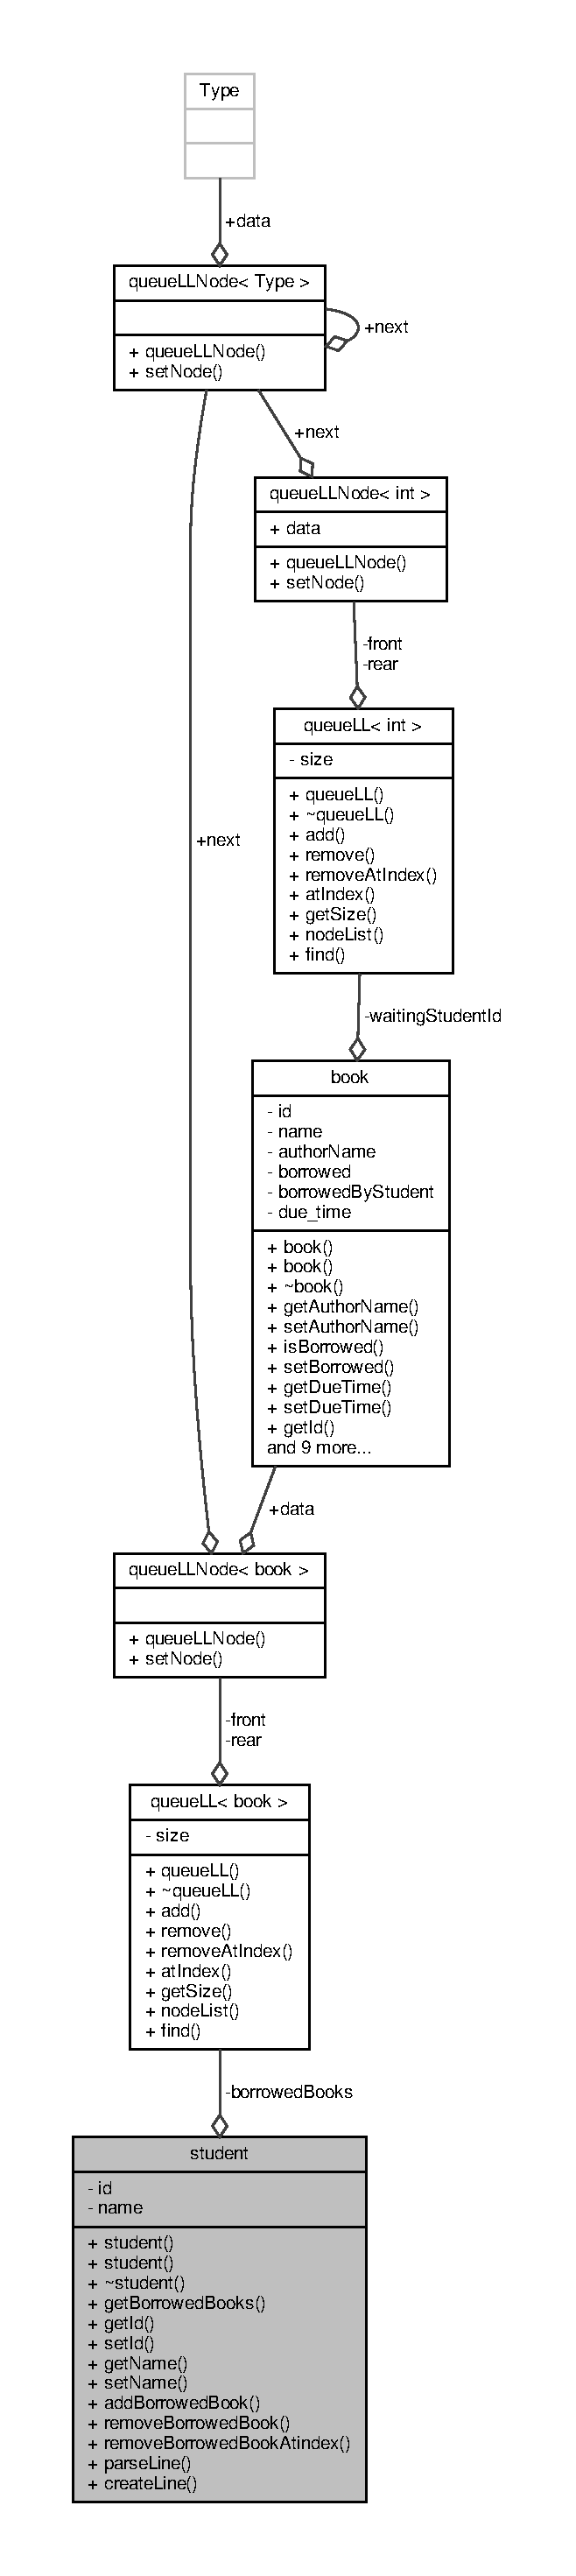
\includegraphics[height=550pt]{classstudent__coll__graph}
\end{center}
\end{figure}
\subsection*{Public Member Functions}
\begin{DoxyCompactItemize}
\item 
\hyperlink{classstudent_a12856a6274dafe06723815e464b6a336}{student} (int i, std\+::string n)
\item 
\hyperlink{classstudent_a9614bbb1bed8ee2aea8aab60fe58494b}{student} ()
\item 
virtual \hyperlink{classstudent_a102d321793438dd827305764bf59f86c}{$\sim$student} ()
\item 
\hyperlink{classqueue_l_l}{queue\+LL}$<$ \hyperlink{classbook}{book} $>$ $\ast$ \hyperlink{classstudent_a27120d590ee93cc80c5b9d72d91a2eb3}{get\+Borrowed\+Books} () const
\item 
int \hyperlink{classstudent_a718b1fdd02dd1ed06110f9e0e7ec7720}{get\+Id} () const
\item 
void \hyperlink{classstudent_abda32701d8741f07e9aa45d339a122ff}{set\+Id} (int \hyperlink{classstudent_a8215d11b0d1adc77e0808a0ff4d0f6a2}{id})
\item 
const std\+::string \& \hyperlink{classstudent_aeeeae15e9a049b1e0973f91bd55fd78b}{get\+Name} () const
\item 
void \hyperlink{classstudent_a9e5279d275d68557215edd499c15b0a2}{set\+Name} (const std\+::string \&\hyperlink{classstudent_a8bba46a454eaecf8619a68c4c38c7b8d}{name})
\item 
void \hyperlink{classstudent_af02c927727b890c189a4641f01185bcc}{add\+Borrowed\+Book} (\hyperlink{classbook}{book} $\ast$item)
\item 
void \hyperlink{classstudent_ab98c4cb9d85152c3abd2b5d4255b8271}{remove\+Borrowed\+Book} ()
\item 
void \hyperlink{classstudent_a5387f0131233065383ca141ddec50de6}{remove\+Borrowed\+Book\+Atindex} (int index)
\item 
bool \hyperlink{classstudent_a73c407020ea392b45dc9ff9babc0850b}{parse\+Line} (std\+::string \&line, \hyperlink{class_book_handler}{Book\+Handler} \&\hyperlink{_library_mananagement_system_8cpp_a2945b7618a199e1ba93546310a14a75a}{books})
\item 
void \hyperlink{classstudent_a4bc363a59fc8b14d81e8e5e0d2326444}{create\+Line} (std\+::string \&line)
\end{DoxyCompactItemize}
\subsection*{Private Attributes}
\begin{DoxyCompactItemize}
\item 
int \hyperlink{classstudent_a8215d11b0d1adc77e0808a0ff4d0f6a2}{id}
\item 
std\+::string \hyperlink{classstudent_a8bba46a454eaecf8619a68c4c38c7b8d}{name}
\item 
\hyperlink{classqueue_l_l}{queue\+LL}$<$ \hyperlink{classbook}{book} $>$ $\ast$ \hyperlink{classstudent_ab477f6c1525709586ea41364dc8c568b}{borrowed\+Books}
\end{DoxyCompactItemize}
\subsection*{Friends}
\begin{DoxyCompactItemize}
\item 
std\+::ostream \& \hyperlink{classstudent_a73f5ef786ecabf4118c6606f42829606}{operator$<$$<$} (std\+::ostream \&out, const \hyperlink{classstudent}{student} \&st)
\item 
bool \hyperlink{classstudent_aaaddafca542c39f7442b1807ba5600c3}{operator!=} (const \hyperlink{classstudent}{student} \&s1, const \hyperlink{classstudent}{student} \&s2)
\end{DoxyCompactItemize}


\subsection{Detailed Description}
Class book shows all the functions and members of a student 

Definition at line 21 of file Student.\+h.



\subsection{Constructor \& Destructor Documentation}
\mbox{\Hypertarget{classstudent_a12856a6274dafe06723815e464b6a336}\label{classstudent_a12856a6274dafe06723815e464b6a336}} 
\index{student@{student}!student@{student}}
\index{student@{student}!student@{student}}
\subsubsection{\texorpdfstring{student()}{student()}\hspace{0.1cm}{\footnotesize\ttfamily [1/2]}}
{\footnotesize\ttfamily student\+::student (\begin{DoxyParamCaption}\item[{int}]{i,  }\item[{std\+::string}]{n }\end{DoxyParamCaption})}

constructor function 

Definition at line 11 of file Student.\+cpp.


\begin{DoxyCode}
11                                      \{
12     \textcolor{keywordtype}{id} = i;
13     \hyperlink{classstudent_a8bba46a454eaecf8619a68c4c38c7b8d}{name} =  n;
14     \hyperlink{classstudent_ab477f6c1525709586ea41364dc8c568b}{borrowedBooks} = \textcolor{keyword}{new} \hyperlink{classqueue_l_l}{queueLL<book>}();
15 \}
\end{DoxyCode}
\mbox{\Hypertarget{classstudent_a9614bbb1bed8ee2aea8aab60fe58494b}\label{classstudent_a9614bbb1bed8ee2aea8aab60fe58494b}} 
\index{student@{student}!student@{student}}
\index{student@{student}!student@{student}}
\subsubsection{\texorpdfstring{student()}{student()}\hspace{0.1cm}{\footnotesize\ttfamily [2/2]}}
{\footnotesize\ttfamily student\+::student (\begin{DoxyParamCaption}{ }\end{DoxyParamCaption})}

constructor function 

Definition at line 17 of file Student.\+cpp.


\begin{DoxyCode}
17                   \{
18     \textcolor{keywordtype}{id} = 0;
19     \hyperlink{classstudent_a8bba46a454eaecf8619a68c4c38c7b8d}{name} =  \textcolor{stringliteral}{" "};
20     \hyperlink{classstudent_ab477f6c1525709586ea41364dc8c568b}{borrowedBooks} = \textcolor{keyword}{new} \hyperlink{classqueue_l_l}{queueLL<book>}();
21 \}
\end{DoxyCode}
\mbox{\Hypertarget{classstudent_a102d321793438dd827305764bf59f86c}\label{classstudent_a102d321793438dd827305764bf59f86c}} 
\index{student@{student}!````~student@{$\sim$student}}
\index{````~student@{$\sim$student}!student@{student}}
\subsubsection{\texorpdfstring{$\sim$student()}{~student()}}
{\footnotesize\ttfamily student\+::$\sim$student (\begin{DoxyParamCaption}{ }\end{DoxyParamCaption})\hspace{0.3cm}{\ttfamily [virtual]}}

destructor function 

Definition at line 23 of file Student.\+cpp.


\begin{DoxyCode}
23                   \{
24     \textcolor{keyword}{delete}(\hyperlink{classstudent_ab477f6c1525709586ea41364dc8c568b}{borrowedBooks});
25 \}
\end{DoxyCode}


\subsection{Member Function Documentation}
\mbox{\Hypertarget{classstudent_af02c927727b890c189a4641f01185bcc}\label{classstudent_af02c927727b890c189a4641f01185bcc}} 
\index{student@{student}!add\+Borrowed\+Book@{add\+Borrowed\+Book}}
\index{add\+Borrowed\+Book@{add\+Borrowed\+Book}!student@{student}}
\subsubsection{\texorpdfstring{add\+Borrowed\+Book()}{addBorrowedBook()}}
{\footnotesize\ttfamily void student\+::add\+Borrowed\+Book (\begin{DoxyParamCaption}\item[{\hyperlink{classbook}{book} $\ast$}]{item }\end{DoxyParamCaption})}

function adds a book to the queue of the borrowed books 
\begin{DoxyParams}{Parameters}
{\em item} & pointer to the book \\
\hline
\end{DoxyParams}


Definition at line 31 of file Student.\+cpp.


\begin{DoxyCode}
31                                         \{
32     \hyperlink{classstudent_ab477f6c1525709586ea41364dc8c568b}{borrowedBooks}->\hyperlink{classqueue_l_l_adcbcc26433da2c9d17b6cf0802d1d7d2}{add}(item);
33 \}
\end{DoxyCode}
Here is the call graph for this function\+:
\nopagebreak
\begin{figure}[H]
\begin{center}
\leavevmode
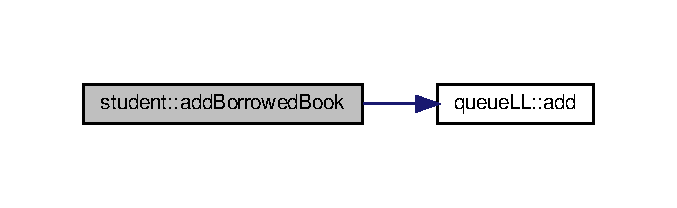
\includegraphics[width=325pt]{classstudent_af02c927727b890c189a4641f01185bcc_cgraph}
\end{center}
\end{figure}
Here is the caller graph for this function\+:
\nopagebreak
\begin{figure}[H]
\begin{center}
\leavevmode
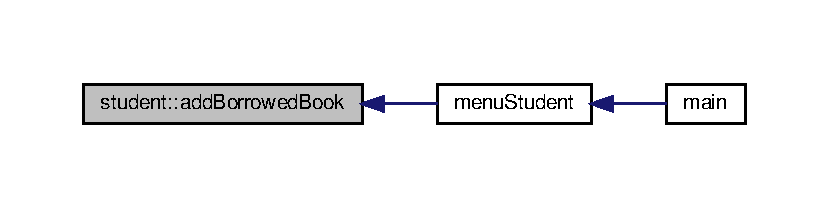
\includegraphics[width=350pt]{classstudent_af02c927727b890c189a4641f01185bcc_icgraph}
\end{center}
\end{figure}
\mbox{\Hypertarget{classstudent_a4bc363a59fc8b14d81e8e5e0d2326444}\label{classstudent_a4bc363a59fc8b14d81e8e5e0d2326444}} 
\index{student@{student}!create\+Line@{create\+Line}}
\index{create\+Line@{create\+Line}!student@{student}}
\subsubsection{\texorpdfstring{create\+Line()}{createLine()}}
{\footnotesize\ttfamily void student\+::create\+Line (\begin{DoxyParamCaption}\item[{std\+::string \&}]{line }\end{DoxyParamCaption})}

function to create line for file 
\begin{DoxyParams}{Parameters}
{\em line} & line that is supposed to write to file \\
\hline
\end{DoxyParams}


Definition at line 111 of file Student.\+cpp.


\begin{DoxyCode}
111                                         \{
112 
113         line = std::to\_string(\textcolor{keywordtype}{id}) + \textcolor{stringliteral}{","} + \hyperlink{classstudent_a8bba46a454eaecf8619a68c4c38c7b8d}{name} + \textcolor{stringliteral}{","} ;
114         \textcolor{keywordflow}{for}(\textcolor{keywordtype}{int} i=0;i<\hyperlink{classstudent_ab477f6c1525709586ea41364dc8c568b}{borrowedBooks}->\hyperlink{classqueue_l_l_a8969feebcb563f0b489bc112422b9563}{getSize}();i++)\{
115             std::string s;
116             \hyperlink{classstudent_ab477f6c1525709586ea41364dc8c568b}{borrowedBooks}->\hyperlink{classqueue_l_l_a6c8873be0f08b3b2e83a24469fbfaa5d}{atIndex}(i)->\hyperlink{classqueue_l_l_node_a20b1170d8c5852b7dc01e56fda4e4206}{data}->\hyperlink{classbook_aea835c54459ec0a4d29d42f2f6f7858d}{createLine}(s);
117             line.append(s);
118             line.append(\textcolor{stringliteral}{"*"});
119         \}
120 \}
\end{DoxyCode}
Here is the call graph for this function\+:
\nopagebreak
\begin{figure}[H]
\begin{center}
\leavevmode
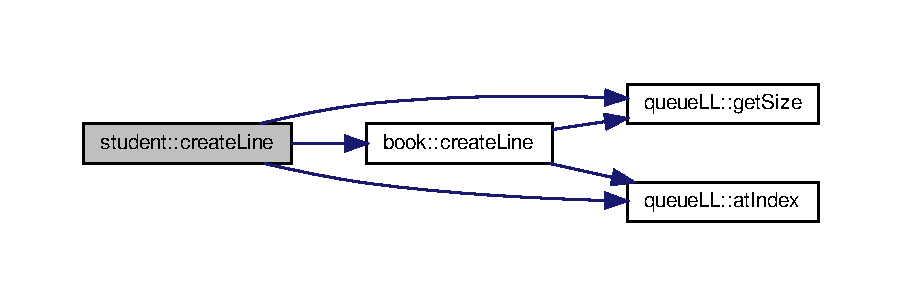
\includegraphics[width=350pt]{classstudent_a4bc363a59fc8b14d81e8e5e0d2326444_cgraph}
\end{center}
\end{figure}
Here is the caller graph for this function\+:
\nopagebreak
\begin{figure}[H]
\begin{center}
\leavevmode
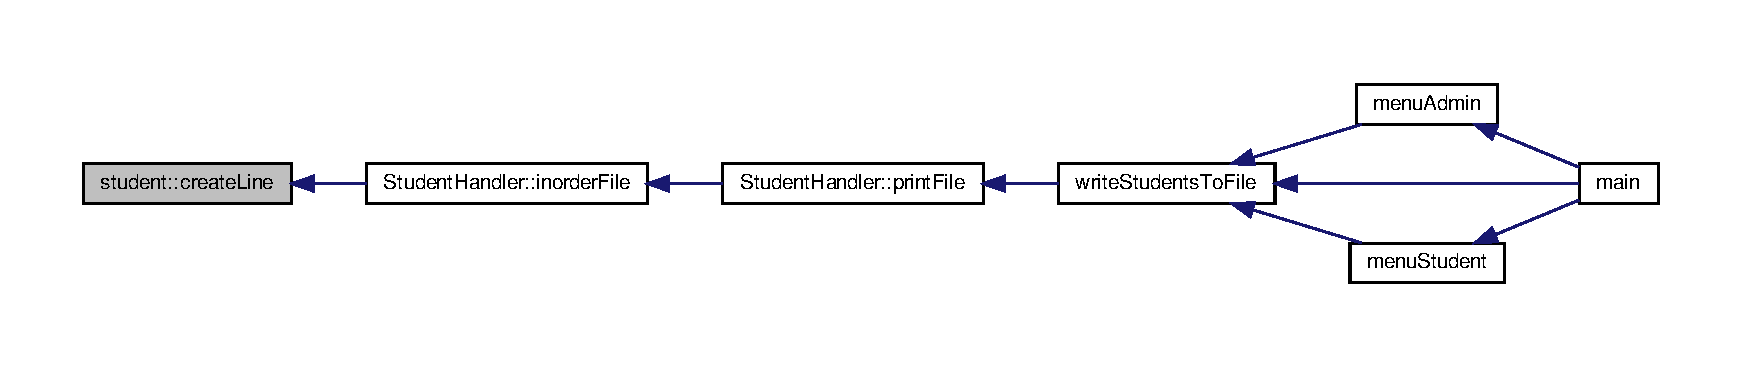
\includegraphics[width=350pt]{classstudent_a4bc363a59fc8b14d81e8e5e0d2326444_icgraph}
\end{center}
\end{figure}
\mbox{\Hypertarget{classstudent_a27120d590ee93cc80c5b9d72d91a2eb3}\label{classstudent_a27120d590ee93cc80c5b9d72d91a2eb3}} 
\index{student@{student}!get\+Borrowed\+Books@{get\+Borrowed\+Books}}
\index{get\+Borrowed\+Books@{get\+Borrowed\+Books}!student@{student}}
\subsubsection{\texorpdfstring{get\+Borrowed\+Books()}{getBorrowedBooks()}}
{\footnotesize\ttfamily \hyperlink{classqueue_l_l}{queue\+LL}$<$ \hyperlink{classbook}{book} $>$ $\ast$ student\+::get\+Borrowed\+Books (\begin{DoxyParamCaption}{ }\end{DoxyParamCaption}) const}

function returns queue of the borrowed books \begin{DoxyReturn}{Returns}
queue of the borrowed books 
\end{DoxyReturn}


Definition at line 27 of file Student.\+cpp.


\begin{DoxyCode}
27                                                \{
28     \textcolor{keywordflow}{return} \hyperlink{classstudent_ab477f6c1525709586ea41364dc8c568b}{borrowedBooks};
29 \}
\end{DoxyCode}
Here is the caller graph for this function\+:
\nopagebreak
\begin{figure}[H]
\begin{center}
\leavevmode
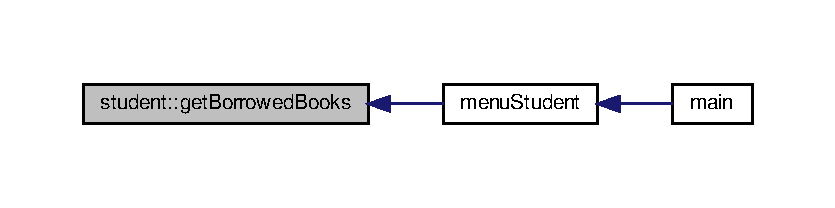
\includegraphics[width=350pt]{classstudent_a27120d590ee93cc80c5b9d72d91a2eb3_icgraph}
\end{center}
\end{figure}
\mbox{\Hypertarget{classstudent_a718b1fdd02dd1ed06110f9e0e7ec7720}\label{classstudent_a718b1fdd02dd1ed06110f9e0e7ec7720}} 
\index{student@{student}!get\+Id@{get\+Id}}
\index{get\+Id@{get\+Id}!student@{student}}
\subsubsection{\texorpdfstring{get\+Id()}{getId()}}
{\footnotesize\ttfamily int student\+::get\+Id (\begin{DoxyParamCaption}{ }\end{DoxyParamCaption}) const}

function returns student id \begin{DoxyReturn}{Returns}
student id 
\end{DoxyReturn}


Definition at line 47 of file Student.\+cpp.


\begin{DoxyCode}
47                          \{
48     \textcolor{keywordflow}{return} \hyperlink{classstudent_a8215d11b0d1adc77e0808a0ff4d0f6a2}{id};
49 \}
\end{DoxyCode}
Here is the caller graph for this function\+:
\nopagebreak
\begin{figure}[H]
\begin{center}
\leavevmode
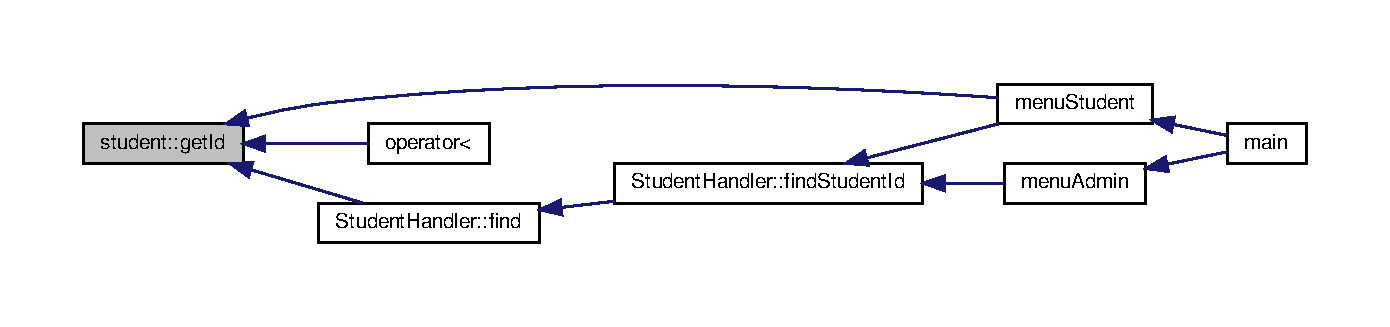
\includegraphics[width=350pt]{classstudent_a718b1fdd02dd1ed06110f9e0e7ec7720_icgraph}
\end{center}
\end{figure}
\mbox{\Hypertarget{classstudent_aeeeae15e9a049b1e0973f91bd55fd78b}\label{classstudent_aeeeae15e9a049b1e0973f91bd55fd78b}} 
\index{student@{student}!get\+Name@{get\+Name}}
\index{get\+Name@{get\+Name}!student@{student}}
\subsubsection{\texorpdfstring{get\+Name()}{getName()}}
{\footnotesize\ttfamily const std\+::string \& student\+::get\+Name (\begin{DoxyParamCaption}{ }\end{DoxyParamCaption}) const}

function returns student name \begin{DoxyReturn}{Returns}
student name 
\end{DoxyReturn}


Definition at line 55 of file Student.\+cpp.


\begin{DoxyCode}
55                                         \{
56     \textcolor{keywordflow}{return} \hyperlink{classstudent_a8bba46a454eaecf8619a68c4c38c7b8d}{name};
57 \}
\end{DoxyCode}
\mbox{\Hypertarget{classstudent_a73c407020ea392b45dc9ff9babc0850b}\label{classstudent_a73c407020ea392b45dc9ff9babc0850b}} 
\index{student@{student}!parse\+Line@{parse\+Line}}
\index{parse\+Line@{parse\+Line}!student@{student}}
\subsubsection{\texorpdfstring{parse\+Line()}{parseLine()}}
{\footnotesize\ttfamily bool student\+::parse\+Line (\begin{DoxyParamCaption}\item[{std\+::string \&}]{line,  }\item[{\hyperlink{class_book_handler}{Book\+Handler} \&}]{books }\end{DoxyParamCaption})}

function to parse line from file 
\begin{DoxyParams}{Parameters}
{\em line} & line that is read from file \\
\hline
\end{DoxyParams}
\begin{DoxyReturn}{Returns}
true, if parse is successful 
\end{DoxyReturn}


Definition at line 80 of file Student.\+cpp.


\begin{DoxyCode}
80                                                             \{
81     \textcolor{keywordtype}{bool} result = \textcolor{keyword}{false};
82 
83     std::stringstream check1(line);
84     std::string intermediate;
85 
86     \textcolor{keywordflow}{if}(std::getline(check1, intermediate, \textcolor{charliteral}{','}))\{\textcolor{comment}{//id}
87 
88         \textcolor{keywordtype}{id} =  std::stoi(intermediate);
89             \textcolor{keywordflow}{if}(std::getline(check1, intermediate, \textcolor{charliteral}{','}))\{\textcolor{comment}{//name}
90             \hyperlink{classstudent_a8bba46a454eaecf8619a68c4c38c7b8d}{name} = intermediate;
91             result = \textcolor{keyword}{true};
92             std::vector <std::string> tokens;
93             \textcolor{keywordflow}{while}(getline(check1, intermediate, \textcolor{charliteral}{'*'}))\{\textcolor{comment}{//borrowedbooks}
94                 tokens.push\_back(intermediate);
95             \}
96             \textcolor{keywordflow}{for}(\textcolor{keywordtype}{int} i = 0; i < tokens.size(); i++)\{
97                 \hyperlink{classbook}{book} * b = \textcolor{keyword}{new} \hyperlink{classbook}{book}();
98                 b->\hyperlink{classbook_acf51be6cb1a1e98d461144e134583c8f}{parseLine}(tokens[i]);
99                 \hyperlink{classbook}{book} * fBook = books.\hyperlink{class_book_handler_aab461b060b38d51586ed043143b4bc68}{findBook}(*b);
100                 \textcolor{keywordflow}{if}(fBook== NULL)\{
101                     std::cout<<\textcolor{stringliteral}{"BOOK ID NOT FOUND!\(\backslash\)n"};
102                 \}
103                 \hyperlink{classstudent_ab477f6c1525709586ea41364dc8c568b}{borrowedBooks}->\hyperlink{classqueue_l_l_adcbcc26433da2c9d17b6cf0802d1d7d2}{add}(fBook);
104                 \textcolor{keyword}{delete}(b);
105             \}
106         \}
107     \}
108     \textcolor{keywordflow}{return} result;
109 \}
\end{DoxyCode}
Here is the call graph for this function\+:
\nopagebreak
\begin{figure}[H]
\begin{center}
\leavevmode
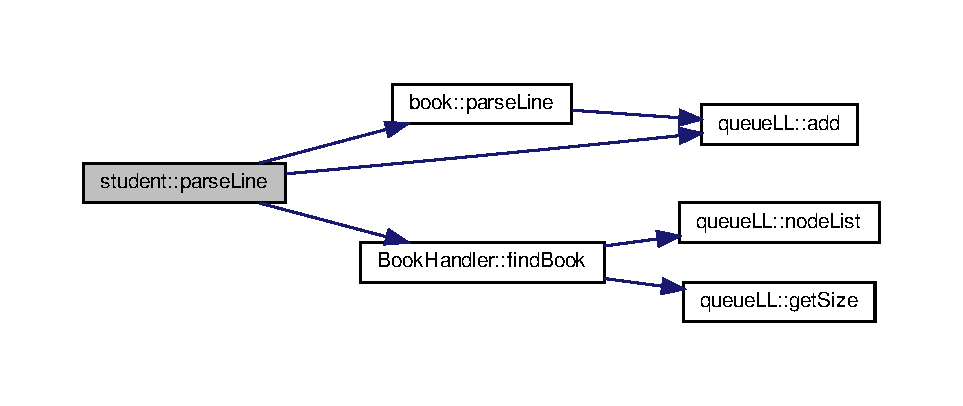
\includegraphics[width=350pt]{classstudent_a73c407020ea392b45dc9ff9babc0850b_cgraph}
\end{center}
\end{figure}
Here is the caller graph for this function\+:
\nopagebreak
\begin{figure}[H]
\begin{center}
\leavevmode
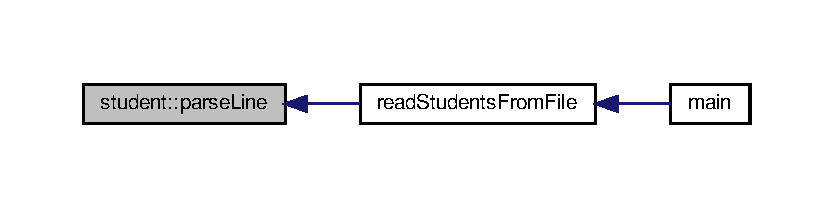
\includegraphics[width=350pt]{classstudent_a73c407020ea392b45dc9ff9babc0850b_icgraph}
\end{center}
\end{figure}
\mbox{\Hypertarget{classstudent_ab98c4cb9d85152c3abd2b5d4255b8271}\label{classstudent_ab98c4cb9d85152c3abd2b5d4255b8271}} 
\index{student@{student}!remove\+Borrowed\+Book@{remove\+Borrowed\+Book}}
\index{remove\+Borrowed\+Book@{remove\+Borrowed\+Book}!student@{student}}
\subsubsection{\texorpdfstring{remove\+Borrowed\+Book()}{removeBorrowedBook()}}
{\footnotesize\ttfamily void student\+::remove\+Borrowed\+Book (\begin{DoxyParamCaption}{ }\end{DoxyParamCaption})}

function removes the first book of the borrowed queue 

Definition at line 34 of file Student.\+cpp.


\begin{DoxyCode}
34                                  \{
35     \hyperlink{classstudent_ab477f6c1525709586ea41364dc8c568b}{borrowedBooks}->\hyperlink{classqueue_l_l_a4204a9db973b69be5824ca2495130b40}{remove}();
36 \}
\end{DoxyCode}
Here is the call graph for this function\+:
\nopagebreak
\begin{figure}[H]
\begin{center}
\leavevmode
\includegraphics[width=350pt]{classstudent_ab98c4cb9d85152c3abd2b5d4255b8271_cgraph}
\end{center}
\end{figure}
\mbox{\Hypertarget{classstudent_a5387f0131233065383ca141ddec50de6}\label{classstudent_a5387f0131233065383ca141ddec50de6}} 
\index{student@{student}!remove\+Borrowed\+Book\+Atindex@{remove\+Borrowed\+Book\+Atindex}}
\index{remove\+Borrowed\+Book\+Atindex@{remove\+Borrowed\+Book\+Atindex}!student@{student}}
\subsubsection{\texorpdfstring{remove\+Borrowed\+Book\+Atindex()}{removeBorrowedBookAtindex()}}
{\footnotesize\ttfamily void student\+::remove\+Borrowed\+Book\+Atindex (\begin{DoxyParamCaption}\item[{int}]{index }\end{DoxyParamCaption})}

function removes the book at location index of the borrowed queue 

Definition at line 38 of file Student.\+cpp.


\begin{DoxyCode}
38                                                  \{
39     \hyperlink{classstudent_ab477f6c1525709586ea41364dc8c568b}{borrowedBooks}->\hyperlink{classqueue_l_l_abe3f175ee8c25c55d18650c5b13297b1}{removeAtIndex}(index);
40 \}
\end{DoxyCode}
Here is the call graph for this function\+:
\nopagebreak
\begin{figure}[H]
\begin{center}
\leavevmode
\includegraphics[width=350pt]{classstudent_a5387f0131233065383ca141ddec50de6_cgraph}
\end{center}
\end{figure}
Here is the caller graph for this function\+:
\nopagebreak
\begin{figure}[H]
\begin{center}
\leavevmode
\includegraphics[width=350pt]{classstudent_a5387f0131233065383ca141ddec50de6_icgraph}
\end{center}
\end{figure}
\mbox{\Hypertarget{classstudent_abda32701d8741f07e9aa45d339a122ff}\label{classstudent_abda32701d8741f07e9aa45d339a122ff}} 
\index{student@{student}!set\+Id@{set\+Id}}
\index{set\+Id@{set\+Id}!student@{student}}
\subsubsection{\texorpdfstring{set\+Id()}{setId()}}
{\footnotesize\ttfamily void student\+::set\+Id (\begin{DoxyParamCaption}\item[{int}]{id }\end{DoxyParamCaption})}

function sets student id 
\begin{DoxyParams}{Parameters}
{\em student} & id \\
\hline
\end{DoxyParams}


Definition at line 51 of file Student.\+cpp.


\begin{DoxyCode}
51                           \{
52     this->\textcolor{keywordtype}{id} = \hyperlink{classstudent_a8215d11b0d1adc77e0808a0ff4d0f6a2}{id};
53 \}
\end{DoxyCode}
\mbox{\Hypertarget{classstudent_a9e5279d275d68557215edd499c15b0a2}\label{classstudent_a9e5279d275d68557215edd499c15b0a2}} 
\index{student@{student}!set\+Name@{set\+Name}}
\index{set\+Name@{set\+Name}!student@{student}}
\subsubsection{\texorpdfstring{set\+Name()}{setName()}}
{\footnotesize\ttfamily void student\+::set\+Name (\begin{DoxyParamCaption}\item[{const std\+::string \&}]{name }\end{DoxyParamCaption})}

function sets student name 
\begin{DoxyParams}{Parameters}
{\em student} & name \\
\hline
\end{DoxyParams}


Definition at line 59 of file Student.\+cpp.


\begin{DoxyCode}
59                                            \{
60     this->\hyperlink{classstudent_a8bba46a454eaecf8619a68c4c38c7b8d}{name} = \hyperlink{classstudent_a8bba46a454eaecf8619a68c4c38c7b8d}{name};
61 \}
\end{DoxyCode}


\subsection{Friends And Related Function Documentation}
\mbox{\Hypertarget{classstudent_aaaddafca542c39f7442b1807ba5600c3}\label{classstudent_aaaddafca542c39f7442b1807ba5600c3}} 
\index{student@{student}!operator"!=@{operator"!=}}
\index{operator"!=@{operator"!=}!student@{student}}
\subsubsection{\texorpdfstring{operator"!=}{operator!=}}
{\footnotesize\ttfamily bool operator!= (\begin{DoxyParamCaption}\item[{const \hyperlink{classstudent}{student} \&}]{s1,  }\item[{const \hyperlink{classstudent}{student} \&}]{s2 }\end{DoxyParamCaption})\hspace{0.3cm}{\ttfamily [friend]}}

function overloads operator != 
\begin{DoxyParams}{Parameters}
{\em out} & output stream \\
\hline
{\em st} & student object \\
\hline
\end{DoxyParams}
\begin{DoxyReturn}{Returns}

\end{DoxyReturn}
\mbox{\Hypertarget{classstudent_a73f5ef786ecabf4118c6606f42829606}\label{classstudent_a73f5ef786ecabf4118c6606f42829606}} 
\index{student@{student}!operator$<$$<$@{operator$<$$<$}}
\index{operator$<$$<$@{operator$<$$<$}!student@{student}}
\subsubsection{\texorpdfstring{operator$<$$<$}{operator<<}}
{\footnotesize\ttfamily std\+::ostream\& operator$<$$<$ (\begin{DoxyParamCaption}\item[{std\+::ostream \&}]{out,  }\item[{const \hyperlink{classstudent}{student} \&}]{st }\end{DoxyParamCaption})\hspace{0.3cm}{\ttfamily [friend]}}

function overloads operator $<$$<$ 
\begin{DoxyParams}{Parameters}
{\em out} & output stream \\
\hline
{\em st} & student object \\
\hline
\end{DoxyParams}
\begin{DoxyReturn}{Returns}

\end{DoxyReturn}


Definition at line 63 of file Student.\+cpp.


\begin{DoxyCode}
63                                                            \{
64     \textcolor{keywordflow}{if}(st.\hyperlink{classstudent_ab477f6c1525709586ea41364dc8c568b}{borrowedBooks}->\hyperlink{classqueue_l_l_a8969feebcb563f0b489bc112422b9563}{getSize}()>0)\{
65         \textcolor{keywordflow}{return} out <<\textcolor{stringliteral}{"STUDENT id="}<< st.\hyperlink{classstudent_a8215d11b0d1adc77e0808a0ff4d0f6a2}{id} << \textcolor{stringliteral}{" name="} <<st.\hyperlink{classstudent_a8bba46a454eaecf8619a68c4c38c7b8d}{name} <<
66                 \textcolor{stringliteral}{" \{list of borrowed books:\(\backslash\)n"}<<*(st.\hyperlink{classstudent_ab477f6c1525709586ea41364dc8c568b}{borrowedBooks})<<\textcolor{stringliteral}{"\}\(\backslash\)n"};
67     \}
68     \textcolor{keywordflow}{else}\{
69         \textcolor{keywordflow}{return} out <<\textcolor{stringliteral}{"STUDENT id="}<< st.\hyperlink{classstudent_a8215d11b0d1adc77e0808a0ff4d0f6a2}{id} << \textcolor{stringliteral}{" name="} <<st.\hyperlink{classstudent_a8bba46a454eaecf8619a68c4c38c7b8d}{name} << \textcolor{stringliteral}{" , student did not borrow a book
      \(\backslash\)n "};
70     \}
71 \}
\end{DoxyCode}


\subsection{Member Data Documentation}
\mbox{\Hypertarget{classstudent_ab477f6c1525709586ea41364dc8c568b}\label{classstudent_ab477f6c1525709586ea41364dc8c568b}} 
\index{student@{student}!borrowed\+Books@{borrowed\+Books}}
\index{borrowed\+Books@{borrowed\+Books}!student@{student}}
\subsubsection{\texorpdfstring{borrowed\+Books}{borrowedBooks}}
{\footnotesize\ttfamily \hyperlink{classqueue_l_l}{queue\+LL}$<$\hyperlink{classbook}{book}$>$$\ast$ student\+::borrowed\+Books\hspace{0.3cm}{\ttfamily [private]}}

queue of borrowed books 

Definition at line 111 of file Student.\+h.

\mbox{\Hypertarget{classstudent_a8215d11b0d1adc77e0808a0ff4d0f6a2}\label{classstudent_a8215d11b0d1adc77e0808a0ff4d0f6a2}} 
\index{student@{student}!id@{id}}
\index{id@{id}!student@{student}}
\subsubsection{\texorpdfstring{id}{id}}
{\footnotesize\ttfamily int student\+::id\hspace{0.3cm}{\ttfamily [private]}}

student id 

Definition at line 103 of file Student.\+h.

\mbox{\Hypertarget{classstudent_a8bba46a454eaecf8619a68c4c38c7b8d}\label{classstudent_a8bba46a454eaecf8619a68c4c38c7b8d}} 
\index{student@{student}!name@{name}}
\index{name@{name}!student@{student}}
\subsubsection{\texorpdfstring{name}{name}}
{\footnotesize\ttfamily std\+::string student\+::name\hspace{0.3cm}{\ttfamily [private]}}

student name 

Definition at line 107 of file Student.\+h.



The documentation for this class was generated from the following files\+:\begin{DoxyCompactItemize}
\item 
src/\hyperlink{_student_8h}{Student.\+h}\item 
src/\hyperlink{_student_8cpp}{Student.\+cpp}\end{DoxyCompactItemize}

\hypertarget{class_student_handler}{}\section{Student\+Handler Class Reference}
\label{class_student_handler}\index{Student\+Handler@{Student\+Handler}}


{\ttfamily \#include $<$Student\+Handler.\+h$>$}



Collaboration diagram for Student\+Handler\+:
\nopagebreak
\begin{figure}[H]
\begin{center}
\leavevmode
\includegraphics[height=550pt]{class_student_handler__coll__graph}
\end{center}
\end{figure}
\subsection*{Public Member Functions}
\begin{DoxyCompactItemize}
\item 
\hyperlink{class_student_handler_a789f9be791a4ada717975e9361f5c967}{Student\+Handler} ()
\item 
virtual \hyperlink{class_student_handler_a1ad6892062e41ea9d5ac1ddf5cdf64c2}{$\sim$\+Student\+Handler} ()
\item 
void \hyperlink{class_student_handler_ae7219f3612d49a8bda1cb14c48557b37}{add\+Student} (int id, std\+::string name)
\item 
void \hyperlink{class_student_handler_a1d0e1f3e8383c38d5c9c5781fb8ce82d}{add\+Student} (\hyperlink{classstudent}{student} $\ast$temp)
\item 
\hyperlink{classstudent}{student} $\ast$ \hyperlink{class_student_handler_ad54072af22b0b84e677af69426ed0bff}{find\+Student\+Id} (int index)
\item 
void \hyperlink{class_student_handler_a08899a7b8ca38541605c564c572d72ef}{print} ()
\item 
void \hyperlink{class_student_handler_a8049bb821d2a0a951600ab79c6ee4e27}{print\+File} (std\+::ofstream \&\hyperlink{_library_mananagement_system_8cpp_a2e073350989a922d101f00447e52dfc6}{ou\+File\+Student})
\end{DoxyCompactItemize}
\subsection*{Private Member Functions}
\begin{DoxyCompactItemize}
\item 
\hyperlink{classstudent}{student} $\ast$ \hyperlink{class_student_handler_a366b1628971d8b8ae437a87978e26e8a}{find} (const \hyperlink{class_node}{Node}$<$ \hyperlink{classstudent}{student} $>$ $\ast$node, int id)
\item 
void \hyperlink{class_student_handler_a9caee269c1ef9b34af2eeb0452a0cabb}{inorder} (const \hyperlink{class_node}{Node}$<$ \hyperlink{classstudent}{student} $>$ $\ast$tmp)
\item 
void \hyperlink{class_student_handler_a61f541e2aa02759a3213a9bceecf125c}{inorder\+File} (const \hyperlink{class_node}{Node}$<$ \hyperlink{classstudent}{student} $>$ $\ast$tmp, std\+::ofstream \&\hyperlink{_library_mananagement_system_8cpp_a2e073350989a922d101f00447e52dfc6}{ou\+File\+Student})
\end{DoxyCompactItemize}
\subsection*{Private Attributes}
\begin{DoxyCompactItemize}
\item 
\hyperlink{class_binary_tree}{Binary\+Tree}$<$ \hyperlink{classstudent}{student} $>$ $\ast$ \hyperlink{class_student_handler_a7141eccd57a30aa140e5b4e92b0939ea}{student\+Tree}
\end{DoxyCompactItemize}


\subsection{Detailed Description}
Class handles the list of the students 

Definition at line 18 of file Student\+Handler.\+h.



\subsection{Constructor \& Destructor Documentation}
\mbox{\Hypertarget{class_student_handler_a789f9be791a4ada717975e9361f5c967}\label{class_student_handler_a789f9be791a4ada717975e9361f5c967}} 
\index{Student\+Handler@{Student\+Handler}!Student\+Handler@{Student\+Handler}}
\index{Student\+Handler@{Student\+Handler}!Student\+Handler@{Student\+Handler}}
\subsubsection{\texorpdfstring{Student\+Handler()}{StudentHandler()}}
{\footnotesize\ttfamily Student\+Handler\+::\+Student\+Handler (\begin{DoxyParamCaption}{ }\end{DoxyParamCaption})}

constructor function 

Definition at line 10 of file Student\+Handler.\+cpp.


\begin{DoxyCode}
10                                \{
11     \hyperlink{class_student_handler_a7141eccd57a30aa140e5b4e92b0939ea}{studentTree} = \textcolor{keyword}{new} \hyperlink{class_binary_tree}{BinaryTree<student>}();
12 \}
\end{DoxyCode}
\mbox{\Hypertarget{class_student_handler_a1ad6892062e41ea9d5ac1ddf5cdf64c2}\label{class_student_handler_a1ad6892062e41ea9d5ac1ddf5cdf64c2}} 
\index{Student\+Handler@{Student\+Handler}!````~Student\+Handler@{$\sim$\+Student\+Handler}}
\index{````~Student\+Handler@{$\sim$\+Student\+Handler}!Student\+Handler@{Student\+Handler}}
\subsubsection{\texorpdfstring{$\sim$\+Student\+Handler()}{~StudentHandler()}}
{\footnotesize\ttfamily Student\+Handler\+::$\sim$\+Student\+Handler (\begin{DoxyParamCaption}{ }\end{DoxyParamCaption})\hspace{0.3cm}{\ttfamily [virtual]}}

destructor function 

Definition at line 14 of file Student\+Handler.\+cpp.


\begin{DoxyCode}
14                                 \{
15     \textcolor{keyword}{delete}(\hyperlink{class_student_handler_a7141eccd57a30aa140e5b4e92b0939ea}{studentTree});
16 \}
\end{DoxyCode}


\subsection{Member Function Documentation}
\mbox{\Hypertarget{class_student_handler_ae7219f3612d49a8bda1cb14c48557b37}\label{class_student_handler_ae7219f3612d49a8bda1cb14c48557b37}} 
\index{Student\+Handler@{Student\+Handler}!add\+Student@{add\+Student}}
\index{add\+Student@{add\+Student}!Student\+Handler@{Student\+Handler}}
\subsubsection{\texorpdfstring{add\+Student()}{addStudent()}\hspace{0.1cm}{\footnotesize\ttfamily [1/2]}}
{\footnotesize\ttfamily void Student\+Handler\+::add\+Student (\begin{DoxyParamCaption}\item[{int}]{id,  }\item[{std\+::string}]{name }\end{DoxyParamCaption})}

function to add a student to the list of the students 
\begin{DoxyParams}{Parameters}
{\em id} & student id \\
\hline
{\em name} & student name \\
\hline
\end{DoxyParams}


Definition at line 18 of file Student\+Handler.\+cpp.


\begin{DoxyCode}
18                                                       \{
19     \hyperlink{classstudent}{student} * temp = \textcolor{keyword}{new} \hyperlink{classstudent}{student}(\textcolor{keywordtype}{id}, name);
20     \hyperlink{class_student_handler_a7141eccd57a30aa140e5b4e92b0939ea}{studentTree}->\hyperlink{class_binary_tree_a69ae782d438253d40cbd194737feca17}{insertNode}(temp);
21 \}
\end{DoxyCode}
Here is the call graph for this function\+:
\nopagebreak
\begin{figure}[H]
\begin{center}
\leavevmode
\includegraphics[width=350pt]{class_student_handler_ae7219f3612d49a8bda1cb14c48557b37_cgraph}
\end{center}
\end{figure}
Here is the caller graph for this function\+:
\nopagebreak
\begin{figure}[H]
\begin{center}
\leavevmode
\includegraphics[width=350pt]{class_student_handler_ae7219f3612d49a8bda1cb14c48557b37_icgraph}
\end{center}
\end{figure}
\mbox{\Hypertarget{class_student_handler_a1d0e1f3e8383c38d5c9c5781fb8ce82d}\label{class_student_handler_a1d0e1f3e8383c38d5c9c5781fb8ce82d}} 
\index{Student\+Handler@{Student\+Handler}!add\+Student@{add\+Student}}
\index{add\+Student@{add\+Student}!Student\+Handler@{Student\+Handler}}
\subsubsection{\texorpdfstring{add\+Student()}{addStudent()}\hspace{0.1cm}{\footnotesize\ttfamily [2/2]}}
{\footnotesize\ttfamily void Student\+Handler\+::add\+Student (\begin{DoxyParamCaption}\item[{\hyperlink{classstudent}{student} $\ast$}]{temp }\end{DoxyParamCaption})}

function to add a student to the list of the students 
\begin{DoxyParams}{Parameters}
{\em temp} & student object \\
\hline
\end{DoxyParams}


Definition at line 23 of file Student\+Handler.\+cpp.


\begin{DoxyCode}
23                                               \{
24     \hyperlink{class_student_handler_a7141eccd57a30aa140e5b4e92b0939ea}{studentTree}->\hyperlink{class_binary_tree_a69ae782d438253d40cbd194737feca17}{insertNode}(temp);
25 \}
\end{DoxyCode}
Here is the call graph for this function\+:
\nopagebreak
\begin{figure}[H]
\begin{center}
\leavevmode
\includegraphics[width=350pt]{class_student_handler_a1d0e1f3e8383c38d5c9c5781fb8ce82d_cgraph}
\end{center}
\end{figure}
\mbox{\Hypertarget{class_student_handler_a366b1628971d8b8ae437a87978e26e8a}\label{class_student_handler_a366b1628971d8b8ae437a87978e26e8a}} 
\index{Student\+Handler@{Student\+Handler}!find@{find}}
\index{find@{find}!Student\+Handler@{Student\+Handler}}
\subsubsection{\texorpdfstring{find()}{find()}}
{\footnotesize\ttfamily \hyperlink{classstudent}{student} $\ast$ Student\+Handler\+::find (\begin{DoxyParamCaption}\item[{const \hyperlink{class_node}{Node}$<$ \hyperlink{classstudent}{student} $>$ $\ast$}]{node,  }\item[{int}]{id }\end{DoxyParamCaption})\hspace{0.3cm}{\ttfamily [private]}}

function to find node 
\begin{DoxyParams}{Parameters}
{\em node} & \\
\hline
{\em id} & \\
\hline
\end{DoxyParams}
\begin{DoxyReturn}{Returns}

\end{DoxyReturn}


Definition at line 27 of file Student\+Handler.\+cpp.


\begin{DoxyCode}
27                                                               \{
28     \textcolor{keywordflow}{if} (node == NULL)
29         \textcolor{keywordflow}{return} NULL;
30 
31     \textcolor{keywordflow}{if} (node->\hyperlink{class_node_a8b322cc3cc17b752eb77533493713ddd}{data}->\hyperlink{classstudent_a718b1fdd02dd1ed06110f9e0e7ec7720}{getId}() == id)
32         \textcolor{keywordflow}{return} node->\hyperlink{class_node_a8b322cc3cc17b752eb77533493713ddd}{data};
33 
34     \hyperlink{classstudent}{student} * resultL = \hyperlink{class_student_handler_a366b1628971d8b8ae437a87978e26e8a}{find}(node->\hyperlink{class_node_abb08a8b3137dd8fc8874348a439e01b4}{left}, \textcolor{keywordtype}{id});
35     \textcolor{keywordflow}{if}(resultL != NULL) \textcolor{keywordflow}{return} resultL;
36 
37     \textcolor{keywordflow}{return} \hyperlink{class_student_handler_a366b1628971d8b8ae437a87978e26e8a}{find}(node->\hyperlink{class_node_a34452c0684d3cb1590406ad201b43e65}{right}, \textcolor{keywordtype}{id});
38 \}
\end{DoxyCode}
Here is the call graph for this function\+:
\nopagebreak
\begin{figure}[H]
\begin{center}
\leavevmode
\includegraphics[width=299pt]{class_student_handler_a366b1628971d8b8ae437a87978e26e8a_cgraph}
\end{center}
\end{figure}
Here is the caller graph for this function\+:
\nopagebreak
\begin{figure}[H]
\begin{center}
\leavevmode
\includegraphics[width=350pt]{class_student_handler_a366b1628971d8b8ae437a87978e26e8a_icgraph}
\end{center}
\end{figure}
\mbox{\Hypertarget{class_student_handler_ad54072af22b0b84e677af69426ed0bff}\label{class_student_handler_ad54072af22b0b84e677af69426ed0bff}} 
\index{Student\+Handler@{Student\+Handler}!find\+Student\+Id@{find\+Student\+Id}}
\index{find\+Student\+Id@{find\+Student\+Id}!Student\+Handler@{Student\+Handler}}
\subsubsection{\texorpdfstring{find\+Student\+Id()}{findStudentId()}}
{\footnotesize\ttfamily \hyperlink{classstudent}{student} $\ast$ Student\+Handler\+::find\+Student\+Id (\begin{DoxyParamCaption}\item[{int}]{index }\end{DoxyParamCaption})}

function to find id of the student at location index of the books list 
\begin{DoxyParams}{Parameters}
{\em index} & \\
\hline
\end{DoxyParams}
\begin{DoxyReturn}{Returns}
\+: pointer to the found student 
\end{DoxyReturn}


Definition at line 40 of file Student\+Handler.\+cpp.


\begin{DoxyCode}
40                                              \{
41 
42     \textcolor{keywordflow}{if}(\hyperlink{class_student_handler_a7141eccd57a30aa140e5b4e92b0939ea}{studentTree}->\hyperlink{class_binary_tree_a9ee0cf09781cf2ecc471aacc61848dde}{getRoot}() == 0)\{
43 \textcolor{comment}{//      std::cout<<"No student is added to the tree";}
44         \textcolor{keywordflow}{return} NULL;
45     \}
46     \textcolor{keywordflow}{else} \{
47         \textcolor{keywordflow}{return} \hyperlink{class_student_handler_a366b1628971d8b8ae437a87978e26e8a}{find}(\hyperlink{class_student_handler_a7141eccd57a30aa140e5b4e92b0939ea}{studentTree}->\hyperlink{class_binary_tree_a9ee0cf09781cf2ecc471aacc61848dde}{getRoot}(), id);
48     \}
49 \}
\end{DoxyCode}
Here is the call graph for this function\+:
\nopagebreak
\begin{figure}[H]
\begin{center}
\leavevmode
\includegraphics[width=350pt]{class_student_handler_ad54072af22b0b84e677af69426ed0bff_cgraph}
\end{center}
\end{figure}
Here is the caller graph for this function\+:
\nopagebreak
\begin{figure}[H]
\begin{center}
\leavevmode
\includegraphics[width=350pt]{class_student_handler_ad54072af22b0b84e677af69426ed0bff_icgraph}
\end{center}
\end{figure}
\mbox{\Hypertarget{class_student_handler_a9caee269c1ef9b34af2eeb0452a0cabb}\label{class_student_handler_a9caee269c1ef9b34af2eeb0452a0cabb}} 
\index{Student\+Handler@{Student\+Handler}!inorder@{inorder}}
\index{inorder@{inorder}!Student\+Handler@{Student\+Handler}}
\subsubsection{\texorpdfstring{inorder()}{inorder()}}
{\footnotesize\ttfamily void Student\+Handler\+::inorder (\begin{DoxyParamCaption}\item[{const \hyperlink{class_node}{Node}$<$ \hyperlink{classstudent}{student} $>$ $\ast$}]{tmp }\end{DoxyParamCaption})\hspace{0.3cm}{\ttfamily [private]}}

function to traverse binary tree of the list of the students inorder 
\begin{DoxyParams}{Parameters}
{\em tmp} & \\
\hline
\end{DoxyParams}


Definition at line 51 of file Student\+Handler.\+cpp.


\begin{DoxyCode}
51                                                      \{
52         \textcolor{keywordflow}{if}(tmp->\hyperlink{class_node_abb08a8b3137dd8fc8874348a439e01b4}{left}!= 0)
53             \hyperlink{class_student_handler_a9caee269c1ef9b34af2eeb0452a0cabb}{inorder}(tmp->\hyperlink{class_node_abb08a8b3137dd8fc8874348a439e01b4}{left});
54         std::cout<<*(tmp->\hyperlink{class_node_a8b322cc3cc17b752eb77533493713ddd}{data}) << \textcolor{stringliteral}{"\(\backslash\)n"};
55         \textcolor{keywordflow}{if}(tmp->\hyperlink{class_node_a34452c0684d3cb1590406ad201b43e65}{right}!= 0)
56             \hyperlink{class_student_handler_a9caee269c1ef9b34af2eeb0452a0cabb}{inorder}(tmp->\hyperlink{class_node_a34452c0684d3cb1590406ad201b43e65}{right});
57     \}
\end{DoxyCode}
Here is the caller graph for this function\+:
\nopagebreak
\begin{figure}[H]
\begin{center}
\leavevmode
\includegraphics[width=350pt]{class_student_handler_a9caee269c1ef9b34af2eeb0452a0cabb_icgraph}
\end{center}
\end{figure}
\mbox{\Hypertarget{class_student_handler_a61f541e2aa02759a3213a9bceecf125c}\label{class_student_handler_a61f541e2aa02759a3213a9bceecf125c}} 
\index{Student\+Handler@{Student\+Handler}!inorder\+File@{inorder\+File}}
\index{inorder\+File@{inorder\+File}!Student\+Handler@{Student\+Handler}}
\subsubsection{\texorpdfstring{inorder\+File()}{inorderFile()}}
{\footnotesize\ttfamily void Student\+Handler\+::inorder\+File (\begin{DoxyParamCaption}\item[{const \hyperlink{class_node}{Node}$<$ \hyperlink{classstudent}{student} $>$ $\ast$}]{tmp,  }\item[{std\+::ofstream \&}]{ou\+File\+Student }\end{DoxyParamCaption})\hspace{0.3cm}{\ttfamily [private]}}

function to traverse binary tree of the list of the students inorder and write in file 
\begin{DoxyParams}{Parameters}
{\em tmp} & \\
\hline
\end{DoxyParams}


Definition at line 67 of file Student\+Handler.\+cpp.


\begin{DoxyCode}
67                                                                                      \{
68         \textcolor{keywordflow}{if}(tmp->\hyperlink{class_node_abb08a8b3137dd8fc8874348a439e01b4}{left}!= 0)
69             \hyperlink{class_student_handler_a61f541e2aa02759a3213a9bceecf125c}{inorderFile}(tmp->\hyperlink{class_node_abb08a8b3137dd8fc8874348a439e01b4}{left}, \hyperlink{_library_mananagement_system_8cpp_a2e073350989a922d101f00447e52dfc6}{ouFileStudent});
70         std::string str;
71         tmp->\hyperlink{class_node_a8b322cc3cc17b752eb77533493713ddd}{data}->\hyperlink{classstudent_a4bc363a59fc8b14d81e8e5e0d2326444}{createLine}(str);
72         \hyperlink{_library_mananagement_system_8cpp_a2e073350989a922d101f00447e52dfc6}{ouFileStudent}<<str<<\textcolor{stringliteral}{"\(\backslash\)n"};
73         \textcolor{keywordflow}{if}(tmp->\hyperlink{class_node_a34452c0684d3cb1590406ad201b43e65}{right}!= 0)
74             \hyperlink{class_student_handler_a61f541e2aa02759a3213a9bceecf125c}{inorderFile}(tmp->\hyperlink{class_node_a34452c0684d3cb1590406ad201b43e65}{right}, \hyperlink{_library_mananagement_system_8cpp_a2e073350989a922d101f00447e52dfc6}{ouFileStudent});
75     \}
\end{DoxyCode}
Here is the call graph for this function\+:
\nopagebreak
\begin{figure}[H]
\begin{center}
\leavevmode
\includegraphics[width=350pt]{class_student_handler_a61f541e2aa02759a3213a9bceecf125c_cgraph}
\end{center}
\end{figure}
Here is the caller graph for this function\+:
\nopagebreak
\begin{figure}[H]
\begin{center}
\leavevmode
\includegraphics[width=350pt]{class_student_handler_a61f541e2aa02759a3213a9bceecf125c_icgraph}
\end{center}
\end{figure}
\mbox{\Hypertarget{class_student_handler_a08899a7b8ca38541605c564c572d72ef}\label{class_student_handler_a08899a7b8ca38541605c564c572d72ef}} 
\index{Student\+Handler@{Student\+Handler}!print@{print}}
\index{print@{print}!Student\+Handler@{Student\+Handler}}
\subsubsection{\texorpdfstring{print()}{print()}}
{\footnotesize\ttfamily void Student\+Handler\+::print (\begin{DoxyParamCaption}{ }\end{DoxyParamCaption})}

function to print the list of the students 

Definition at line 58 of file Student\+Handler.\+cpp.


\begin{DoxyCode}
58                            \{
59     \textcolor{keywordflow}{if}(\hyperlink{class_student_handler_a7141eccd57a30aa140e5b4e92b0939ea}{studentTree}->\hyperlink{class_binary_tree_a9ee0cf09781cf2ecc471aacc61848dde}{getRoot}() == 0)\{
60         std::cout<<\textcolor{stringliteral}{"No student is added to the tree"};
61     \}
62     \textcolor{keywordflow}{else} \{
63          \hyperlink{class_student_handler_a9caee269c1ef9b34af2eeb0452a0cabb}{inorder}(\hyperlink{class_student_handler_a7141eccd57a30aa140e5b4e92b0939ea}{studentTree}->\hyperlink{class_binary_tree_a9ee0cf09781cf2ecc471aacc61848dde}{getRoot}());
64     \}
65 \}
\end{DoxyCode}
Here is the call graph for this function\+:
\nopagebreak
\begin{figure}[H]
\begin{center}
\leavevmode
\includegraphics[width=344pt]{class_student_handler_a08899a7b8ca38541605c564c572d72ef_cgraph}
\end{center}
\end{figure}
Here is the caller graph for this function\+:
\nopagebreak
\begin{figure}[H]
\begin{center}
\leavevmode
\includegraphics[width=350pt]{class_student_handler_a08899a7b8ca38541605c564c572d72ef_icgraph}
\end{center}
\end{figure}
\mbox{\Hypertarget{class_student_handler_a8049bb821d2a0a951600ab79c6ee4e27}\label{class_student_handler_a8049bb821d2a0a951600ab79c6ee4e27}} 
\index{Student\+Handler@{Student\+Handler}!print\+File@{print\+File}}
\index{print\+File@{print\+File}!Student\+Handler@{Student\+Handler}}
\subsubsection{\texorpdfstring{print\+File()}{printFile()}}
{\footnotesize\ttfamily void Student\+Handler\+::print\+File (\begin{DoxyParamCaption}\item[{std\+::ofstream \&}]{ou\+File\+Student }\end{DoxyParamCaption})}

function to print the list of the students to the file 

Definition at line 76 of file Student\+Handler.\+cpp.


\begin{DoxyCode}
76                                                          \{
77     \textcolor{keywordflow}{if}(\hyperlink{class_student_handler_a7141eccd57a30aa140e5b4e92b0939ea}{studentTree}->\hyperlink{class_binary_tree_a9ee0cf09781cf2ecc471aacc61848dde}{getRoot}() == 0)\{
78         std::cout<<\textcolor{stringliteral}{"No student is added to the tree"};
79     \}
80     \textcolor{keywordflow}{else} \{
81         \hyperlink{class_student_handler_a61f541e2aa02759a3213a9bceecf125c}{inorderFile}(\hyperlink{class_student_handler_a7141eccd57a30aa140e5b4e92b0939ea}{studentTree}->\hyperlink{class_binary_tree_a9ee0cf09781cf2ecc471aacc61848dde}{getRoot}(),
      \hyperlink{_library_mananagement_system_8cpp_a2e073350989a922d101f00447e52dfc6}{ouFileStudent});
82     \}
83 \}
\end{DoxyCode}
Here is the call graph for this function\+:
\nopagebreak
\begin{figure}[H]
\begin{center}
\leavevmode
\includegraphics[width=350pt]{class_student_handler_a8049bb821d2a0a951600ab79c6ee4e27_cgraph}
\end{center}
\end{figure}
Here is the caller graph for this function\+:
\nopagebreak
\begin{figure}[H]
\begin{center}
\leavevmode
\includegraphics[width=350pt]{class_student_handler_a8049bb821d2a0a951600ab79c6ee4e27_icgraph}
\end{center}
\end{figure}


\subsection{Member Data Documentation}
\mbox{\Hypertarget{class_student_handler_a7141eccd57a30aa140e5b4e92b0939ea}\label{class_student_handler_a7141eccd57a30aa140e5b4e92b0939ea}} 
\index{Student\+Handler@{Student\+Handler}!student\+Tree@{student\+Tree}}
\index{student\+Tree@{student\+Tree}!Student\+Handler@{Student\+Handler}}
\subsubsection{\texorpdfstring{student\+Tree}{studentTree}}
{\footnotesize\ttfamily \hyperlink{class_binary_tree}{Binary\+Tree}$<$\hyperlink{classstudent}{student}$>$$\ast$ Student\+Handler\+::student\+Tree\hspace{0.3cm}{\ttfamily [private]}}

list of the students is kept in a queue 

Definition at line 59 of file Student\+Handler.\+h.



The documentation for this class was generated from the following files\+:\begin{DoxyCompactItemize}
\item 
src/\hyperlink{_student_handler_8h}{Student\+Handler.\+h}\item 
src/\hyperlink{_student_handler_8cpp}{Student\+Handler.\+cpp}\end{DoxyCompactItemize}

\chapter{File Documentation}
\hypertarget{_book_8d}{}\section{Debug/src/\+Book.d File Reference}
\label{_book_8d}\index{Debug/src/\+Book.\+d@{Debug/src/\+Book.\+d}}

\hypertarget{_book_handler_8d}{}\section{Debug/src/\+Book\+Handler.d File Reference}
\label{_book_handler_8d}\index{Debug/src/\+Book\+Handler.\+d@{Debug/src/\+Book\+Handler.\+d}}

\hypertarget{_library_mananagement_system_8d}{}\section{Debug/src/\+Library\+Mananagement\+System.d File Reference}
\label{_library_mananagement_system_8d}\index{Debug/src/\+Library\+Mananagement\+System.\+d@{Debug/src/\+Library\+Mananagement\+System.\+d}}

\hypertarget{_student_8d}{}\section{Debug/src/\+Student.d File Reference}
\label{_student_8d}\index{Debug/src/\+Student.\+d@{Debug/src/\+Student.\+d}}

\hypertarget{_student_handler_8d}{}\section{Debug/src/\+Student\+Handler.d File Reference}
\label{_student_handler_8d}\index{Debug/src/\+Student\+Handler.\+d@{Debug/src/\+Student\+Handler.\+d}}

\hypertarget{_binary_tree_8h}{}\section{src/\+Binary\+Tree.h File Reference}
\label{_binary_tree_8h}\index{src/\+Binary\+Tree.\+h@{src/\+Binary\+Tree.\+h}}
{\ttfamily \#include \char`\"{}Queue\+L\+L.\+h\char`\"{}}\newline
Include dependency graph for Binary\+Tree.\+h\+:
\nopagebreak
\begin{figure}[H]
\begin{center}
\leavevmode
\includegraphics[width=169pt]{_binary_tree_8h__incl}
\end{center}
\end{figure}
This graph shows which files directly or indirectly include this file\+:
\nopagebreak
\begin{figure}[H]
\begin{center}
\leavevmode
\includegraphics[width=350pt]{_binary_tree_8h__dep__incl}
\end{center}
\end{figure}
\subsection*{Classes}
\begin{DoxyCompactItemize}
\item 
class \hyperlink{class_node}{Node$<$ Type $>$}
\item 
class \hyperlink{class_binary_tree}{Binary\+Tree$<$ Type $>$}
\end{DoxyCompactItemize}

\hypertarget{_book_8cpp}{}\section{src/\+Book.cpp File Reference}
\label{_book_8cpp}\index{src/\+Book.\+cpp@{src/\+Book.\+cpp}}
{\ttfamily \#include \char`\"{}Book.\+h\char`\"{}}\newline
Include dependency graph for Book.\+cpp\+:
\nopagebreak
\begin{figure}[H]
\begin{center}
\leavevmode
\includegraphics[width=350pt]{_book_8cpp__incl}
\end{center}
\end{figure}
\subsection*{Functions}
\begin{DoxyCompactItemize}
\item 
std\+::ostream \& \hyperlink{_book_8cpp_a9bd0243ea50c5b8c37ed0d5527f24177}{operator$<$$<$} (std\+::ostream \&out, const \hyperlink{classbook}{book} \&b)
\item 
bool \hyperlink{_book_8cpp_af7856e28b06865a9691d5c7a330633a4}{operator!=} (const \hyperlink{classbook}{book} \&b1, const \hyperlink{classbook}{book} \&b2)
\item 
bool \hyperlink{_book_8cpp_a3d386e1f8255c6b62d9858fb8ff41c86}{operator$<$} (\hyperlink{classbook}{book} \&b1, \hyperlink{classbook}{book} \&b2)
\end{DoxyCompactItemize}


\subsection{Function Documentation}
\mbox{\Hypertarget{_book_8cpp_af7856e28b06865a9691d5c7a330633a4}\label{_book_8cpp_af7856e28b06865a9691d5c7a330633a4}} 
\index{Book.\+cpp@{Book.\+cpp}!operator"!=@{operator"!=}}
\index{operator"!=@{operator"!=}!Book.\+cpp@{Book.\+cpp}}
\subsubsection{\texorpdfstring{operator"!=()}{operator!=()}}
{\footnotesize\ttfamily bool operator!= (\begin{DoxyParamCaption}\item[{const \hyperlink{classbook}{book} \&}]{b1,  }\item[{const \hyperlink{classbook}{book} \&}]{b2 }\end{DoxyParamCaption})}

function overloads operator != (not equal) 
\begin{DoxyParams}{Parameters}
{\em b1} & first book object \\
\hline
{\em b2} & second book object \\
\hline
\end{DoxyParams}
\begin{DoxyReturn}{Returns}

\end{DoxyReturn}


Definition at line 156 of file Book.\+cpp.


\begin{DoxyCode}
156                                                  \{
157     \textcolor{keywordflow}{if}(b1.\hyperlink{classbook_ad8bf54b50c72af3827823c04d724d824}{id}!=b2.\hyperlink{classbook_ad8bf54b50c72af3827823c04d724d824}{id} || b1.\hyperlink{classbook_a5eabc1c1c5abff26997bec3d41f90d9e}{name}!=b2.\hyperlink{classbook_a5eabc1c1c5abff26997bec3d41f90d9e}{name} || b1.\hyperlink{classbook_a21b2962c6227818732db27f12121b732}{authorName}!=b2.
      \hyperlink{classbook_a21b2962c6227818732db27f12121b732}{authorName})
158         \textcolor{keywordflow}{return} \textcolor{keyword}{true};
159     \textcolor{keywordflow}{else}
160         \textcolor{keywordflow}{return} \textcolor{keyword}{false};
161 \}
\end{DoxyCode}
\mbox{\Hypertarget{_book_8cpp_a3d386e1f8255c6b62d9858fb8ff41c86}\label{_book_8cpp_a3d386e1f8255c6b62d9858fb8ff41c86}} 
\index{Book.\+cpp@{Book.\+cpp}!operator$<$@{operator$<$}}
\index{operator$<$@{operator$<$}!Book.\+cpp@{Book.\+cpp}}
\subsubsection{\texorpdfstring{operator$<$()}{operator<()}}
{\footnotesize\ttfamily bool operator$<$ (\begin{DoxyParamCaption}\item[{\hyperlink{classbook}{book} \&}]{b1,  }\item[{\hyperlink{classbook}{book} \&}]{b2 }\end{DoxyParamCaption})}

overload operator $<$ 
\begin{DoxyParams}{Parameters}
{\em b1} & first book object \\
\hline
{\em b2} & first book object \\
\hline
\end{DoxyParams}
\begin{DoxyReturn}{Returns}
true, if due time b1 is smaller than due time b2 
\end{DoxyReturn}


Definition at line 163 of file Book.\+cpp.


\begin{DoxyCode}
163                                       \{
164     time\_t t1 = mktime(&(b1.\hyperlink{classbook_abf72d9a32cdadee632df5a626dbe33b8}{due\_time}));
165     time\_t t2 = mktime(&(b2.\hyperlink{classbook_abf72d9a32cdadee632df5a626dbe33b8}{due\_time}));
166     \textcolor{keywordtype}{double} diffSecs = difftime(t1, t2);
167     \textcolor{keywordflow}{if}(diffSecs<0 )
168         \textcolor{keywordflow}{return} \textcolor{keyword}{true};
169     \textcolor{keywordflow}{else}
170         \textcolor{keywordflow}{return} \textcolor{keyword}{false};
171 \}
\end{DoxyCode}
\mbox{\Hypertarget{_book_8cpp_a9bd0243ea50c5b8c37ed0d5527f24177}\label{_book_8cpp_a9bd0243ea50c5b8c37ed0d5527f24177}} 
\index{Book.\+cpp@{Book.\+cpp}!operator$<$$<$@{operator$<$$<$}}
\index{operator$<$$<$@{operator$<$$<$}!Book.\+cpp@{Book.\+cpp}}
\subsubsection{\texorpdfstring{operator$<$$<$()}{operator<<()}}
{\footnotesize\ttfamily std\+::ostream\& operator$<$$<$ (\begin{DoxyParamCaption}\item[{std\+::ostream \&}]{out,  }\item[{const \hyperlink{classbook}{book} \&}]{b }\end{DoxyParamCaption})}

function overloads operator $<$$<$ 
\begin{DoxyParams}{Parameters}
{\em out} & output stream \\
\hline
{\em b} & book object \\
\hline
\end{DoxyParams}
\begin{DoxyReturn}{Returns}

\end{DoxyReturn}


Definition at line 133 of file Book.\+cpp.


\begin{DoxyCode}
133                                                         \{
134      std::string tmp= b.\hyperlink{classbook_ab745520ed537e69bde6f2e3d7a103276}{borrowed}?\textcolor{stringliteral}{"borrowed "}:\textcolor{stringliteral}{"not borrowed "};
135      \textcolor{keywordflow}{if}(b.\hyperlink{classbook_a40ce04fcfbf99ffdbe7a4e1463588ee5}{waitingStudentId}->\hyperlink{classqueue_l_l_a8969feebcb563f0b489bc112422b9563}{getSize}()>0)
136          \textcolor{keywordflow}{return} out <<\textcolor{stringliteral}{"BOOK id="}<< b.\hyperlink{classbook_ad8bf54b50c72af3827823c04d724d824}{id} << \textcolor{stringliteral}{" name="} << b.\hyperlink{classbook_a5eabc1c1c5abff26997bec3d41f90d9e}{name} << \textcolor{stringliteral}{" author="}
137                  << b.\hyperlink{classbook_a21b2962c6227818732db27f12121b732}{authorName} << \textcolor{stringliteral}{" "}<<tmp << \textcolor{stringliteral}{" due date="}
138                  << b.\hyperlink{classbook_abf72d9a32cdadee632df5a626dbe33b8}{due\_time}.tm\_year<<\textcolor{stringliteral}{"-"}<< b.\hyperlink{classbook_abf72d9a32cdadee632df5a626dbe33b8}{due\_time}.tm\_mon<<\textcolor{stringliteral}{"-"}
139                  << b.\hyperlink{classbook_abf72d9a32cdadee632df5a626dbe33b8}{due\_time}.tm\_mday<<\textcolor{stringliteral}{" "}<< b.\hyperlink{classbook_abf72d9a32cdadee632df5a626dbe33b8}{due\_time}.tm\_hour<<\textcolor{stringliteral}{":"}
140                  << b.\hyperlink{classbook_abf72d9a32cdadee632df5a626dbe33b8}{due\_time}.tm\_min<< \textcolor{stringliteral}{":"}<< b.\hyperlink{classbook_abf72d9a32cdadee632df5a626dbe33b8}{due\_time}.tm\_sec
141                  <<\textcolor{stringliteral}{" waiting students' id="}<< *(b.\hyperlink{classbook_a40ce04fcfbf99ffdbe7a4e1463588ee5}{waitingStudentId})<<\textcolor{stringliteral}{"\(\backslash\)n"};
142      \textcolor{keywordflow}{else}\{
143          \textcolor{keywordflow}{if}( b.\hyperlink{classbook_ab745520ed537e69bde6f2e3d7a103276}{borrowed})
144              \textcolor{keywordflow}{return} out <<\textcolor{stringliteral}{"BOOK id="}<< b.\hyperlink{classbook_ad8bf54b50c72af3827823c04d724d824}{id} << \textcolor{stringliteral}{" name="} << b.\hyperlink{classbook_a5eabc1c1c5abff26997bec3d41f90d9e}{name} << \textcolor{stringliteral}{" author="}
145                      << b.\hyperlink{classbook_a21b2962c6227818732db27f12121b732}{authorName} << \textcolor{stringliteral}{" "}<< tmp << \textcolor{stringliteral}{" due date="}
146                      << b.\hyperlink{classbook_abf72d9a32cdadee632df5a626dbe33b8}{due\_time}.tm\_year<<\textcolor{stringliteral}{"-"}<< b.\hyperlink{classbook_abf72d9a32cdadee632df5a626dbe33b8}{due\_time}.tm\_mon<<\textcolor{stringliteral}{"-"}
147                      << b.\hyperlink{classbook_abf72d9a32cdadee632df5a626dbe33b8}{due\_time}.tm\_mday<<\textcolor{stringliteral}{" "}<< b.\hyperlink{classbook_abf72d9a32cdadee632df5a626dbe33b8}{due\_time}.tm\_hour<<\textcolor{stringliteral}{":"}
148                      << b.\hyperlink{classbook_abf72d9a32cdadee632df5a626dbe33b8}{due\_time}.tm\_min<< \textcolor{stringliteral}{":"}<< b.\hyperlink{classbook_abf72d9a32cdadee632df5a626dbe33b8}{due\_time}.tm\_sec <<\textcolor{stringliteral}{"\(\backslash\)n"};
149          \textcolor{keywordflow}{else}
150              \textcolor{keywordflow}{return} out <<\textcolor{stringliteral}{"BOOK id="}<< b.\hyperlink{classbook_ad8bf54b50c72af3827823c04d724d824}{id} << \textcolor{stringliteral}{" name="} << b.\hyperlink{classbook_a5eabc1c1c5abff26997bec3d41f90d9e}{name} << \textcolor{stringliteral}{" author="}
151                                  << b.\hyperlink{classbook_a21b2962c6227818732db27f12121b732}{authorName} << \textcolor{stringliteral}{" "}<< tmp<<\textcolor{stringliteral}{"\(\backslash\)n"};
152      \}
153 \}
\end{DoxyCode}
Here is the call graph for this function\+:
\nopagebreak
\begin{figure}[H]
\begin{center}
\leavevmode
\includegraphics[width=272pt]{_book_8cpp_a9bd0243ea50c5b8c37ed0d5527f24177_cgraph}
\end{center}
\end{figure}

\hypertarget{_book_8h}{}\section{src/\+Book.h File Reference}
\label{_book_8h}\index{src/\+Book.\+h@{src/\+Book.\+h}}
{\ttfamily \#include $<$string$>$}\newline
{\ttfamily \#include $<$ctime$>$}\newline
{\ttfamily \#include \char`\"{}Queue\+L\+L.\+h\char`\"{}}\newline
{\ttfamily \#include $<$cstring$>$}\newline
{\ttfamily \#include $<$time.\+h$>$}\newline
{\ttfamily \#include $<$bits/stdc++.\+h$>$}\newline
{\ttfamily \#include $<$vector$>$}\newline
Include dependency graph for Book.\+h\+:
\nopagebreak
\begin{figure}[H]
\begin{center}
\leavevmode
\includegraphics[width=350pt]{_book_8h__incl}
\end{center}
\end{figure}
This graph shows which files directly or indirectly include this file\+:
\nopagebreak
\begin{figure}[H]
\begin{center}
\leavevmode
\includegraphics[width=350pt]{_book_8h__dep__incl}
\end{center}
\end{figure}
\subsection*{Classes}
\begin{DoxyCompactItemize}
\item 
class \hyperlink{classbook}{book}
\end{DoxyCompactItemize}
\subsection*{Variables}
\begin{DoxyCompactItemize}
\item 
static int \hyperlink{_book_8h_a84e48ab264903213f7f7a264da4e867d}{B\+O\+O\+K\+\_\+\+C\+O\+U\+NT} =0
\item 
const int \hyperlink{_book_8h_aded88185ac6dc121bc515c79c54a917a}{B\+O\+R\+R\+O\+W\+\_\+\+T\+I\+ME} = 2
\end{DoxyCompactItemize}


\subsection{Variable Documentation}
\mbox{\Hypertarget{_book_8h_a84e48ab264903213f7f7a264da4e867d}\label{_book_8h_a84e48ab264903213f7f7a264da4e867d}} 
\index{Book.\+h@{Book.\+h}!B\+O\+O\+K\+\_\+\+C\+O\+U\+NT@{B\+O\+O\+K\+\_\+\+C\+O\+U\+NT}}
\index{B\+O\+O\+K\+\_\+\+C\+O\+U\+NT@{B\+O\+O\+K\+\_\+\+C\+O\+U\+NT}!Book.\+h@{Book.\+h}}
\subsubsection{\texorpdfstring{B\+O\+O\+K\+\_\+\+C\+O\+U\+NT}{BOOK\_COUNT}}
{\footnotesize\ttfamily int B\+O\+O\+K\+\_\+\+C\+O\+U\+NT =0\hspace{0.3cm}{\ttfamily [static]}}



Definition at line 19 of file Book.\+h.

\mbox{\Hypertarget{_book_8h_aded88185ac6dc121bc515c79c54a917a}\label{_book_8h_aded88185ac6dc121bc515c79c54a917a}} 
\index{Book.\+h@{Book.\+h}!B\+O\+R\+R\+O\+W\+\_\+\+T\+I\+ME@{B\+O\+R\+R\+O\+W\+\_\+\+T\+I\+ME}}
\index{B\+O\+R\+R\+O\+W\+\_\+\+T\+I\+ME@{B\+O\+R\+R\+O\+W\+\_\+\+T\+I\+ME}!Book.\+h@{Book.\+h}}
\subsubsection{\texorpdfstring{B\+O\+R\+R\+O\+W\+\_\+\+T\+I\+ME}{BORROW\_TIME}}
{\footnotesize\ttfamily const int B\+O\+R\+R\+O\+W\+\_\+\+T\+I\+ME = 2}



Definition at line 20 of file Book.\+h.


\hypertarget{_book_handler_8cpp}{}\section{src/\+Book\+Handler.cpp File Reference}
\label{_book_handler_8cpp}\index{src/\+Book\+Handler.\+cpp@{src/\+Book\+Handler.\+cpp}}
{\ttfamily \#include \char`\"{}Book\+Handler.\+h\char`\"{}}\newline
Include dependency graph for Book\+Handler.\+cpp\+:
\nopagebreak
\begin{figure}[H]
\begin{center}
\leavevmode
\includegraphics[width=350pt]{_book_handler_8cpp__incl}
\end{center}
\end{figure}

\hypertarget{_book_handler_8h}{}\section{src/\+Book\+Handler.h File Reference}
\label{_book_handler_8h}\index{src/\+Book\+Handler.\+h@{src/\+Book\+Handler.\+h}}
{\ttfamily \#include \char`\"{}Book.\+h\char`\"{}}\newline
{\ttfamily \#include \char`\"{}Queue\+L\+L.\+h\char`\"{}}\newline
{\ttfamily \#include $<$fstream$>$}\newline
Include dependency graph for Book\+Handler.\+h\+:
\nopagebreak
\begin{figure}[H]
\begin{center}
\leavevmode
\includegraphics[width=350pt]{_book_handler_8h__incl}
\end{center}
\end{figure}
This graph shows which files directly or indirectly include this file\+:
\nopagebreak
\begin{figure}[H]
\begin{center}
\leavevmode
\includegraphics[width=350pt]{_book_handler_8h__dep__incl}
\end{center}
\end{figure}
\subsection*{Classes}
\begin{DoxyCompactItemize}
\item 
class \hyperlink{class_book_handler}{Book\+Handler}
\end{DoxyCompactItemize}

\hypertarget{_library_mananagement_system_8cpp}{}\section{src/\+Library\+Mananagement\+System.cpp File Reference}
\label{_library_mananagement_system_8cpp}\index{src/\+Library\+Mananagement\+System.\+cpp@{src/\+Library\+Mananagement\+System.\+cpp}}
{\ttfamily \#include $<$iostream$>$}\newline
{\ttfamily \#include $<$stdio.\+h$>$}\newline
{\ttfamily \#include \char`\"{}Student\+Handler.\+h\char`\"{}}\newline
{\ttfamily \#include \char`\"{}Book\+Handler.\+h\char`\"{}}\newline
{\ttfamily \#include $<$fstream$>$}\newline
Include dependency graph for Library\+Mananagement\+System.\+cpp\+:
\nopagebreak
\begin{figure}[H]
\begin{center}
\leavevmode
\includegraphics[width=350pt]{_library_mananagement_system_8cpp__incl}
\end{center}
\end{figure}
\subsection*{Functions}
\begin{DoxyCompactItemize}
\item 
{\footnotesize template$<$typename T $>$ }\\void \hyperlink{_library_mananagement_system_8cpp_a4ba67c6c5f6d58844eece44ff28f38f1}{swap} (T $\ast$a, T $\ast$b)
\item 
{\footnotesize template$<$typename T $>$ }\\int \hyperlink{_library_mananagement_system_8cpp_af3d1a3d711804d29b4172054d6de56fa}{partition} (T $\ast$arr\+List, int start, int end)
\item 
{\footnotesize template$<$typename T $>$ }\\void \hyperlink{_library_mananagement_system_8cpp_ab756bf2cc4974ccab046acfcf41e7a95}{Quicksort} (T $\ast$arr\+List, int start, int end)
\item 
void \hyperlink{_library_mananagement_system_8cpp_a5d29f499bef3936e914ba9b9bd33c52c}{read\+Students\+From\+File} ()
\item 
void \hyperlink{_library_mananagement_system_8cpp_a1489a19670bb87989d92fa0bc667d6f4}{read\+Books\+From\+File} ()
\item 
void \hyperlink{_library_mananagement_system_8cpp_a4553a1ae7185f7dfe1cf9d15b38ad35c}{write\+Students\+To\+File} ()
\item 
void \hyperlink{_library_mananagement_system_8cpp_abbfe09f5b391ad6e6bdb7b48338a54c6}{write\+Books\+To\+File} ()
\item 
void \hyperlink{_library_mananagement_system_8cpp_a36ad170338d7feb540a9ce2f1f8bb1b0}{intro} ()
\item 
void \hyperlink{_library_mananagement_system_8cpp_ae2338f2b60de8c59eaa31a6a285c1fc0}{goodbye} ()
\item 
void \hyperlink{_library_mananagement_system_8cpp_a49fa1336abeb5443d70a08f235af8e61}{menu1} ()
\item 
void \hyperlink{_library_mananagement_system_8cpp_a16202881086f36cce6f9d7878b3bb1f9}{menu\+Admin} ()
\item 
void \hyperlink{_library_mananagement_system_8cpp_a496c74d9e9a86d627304d79618738c57}{menu\+Student} ()
\item 
int \hyperlink{_library_mananagement_system_8cpp_a0ddf1224851353fc92bfbff6f499fa97}{main} (int argc, char $\ast$argv\mbox{[}$\,$\mbox{]})
\end{DoxyCompactItemize}
\subsection*{Variables}
\begin{DoxyCompactItemize}
\item 
\hyperlink{class_student_handler}{Student\+Handler} \hyperlink{_library_mananagement_system_8cpp_a35a6ce1dad360c87455a287284462c1a}{students}
\item 
\hyperlink{class_book_handler}{Book\+Handler} \hyperlink{_library_mananagement_system_8cpp_a2945b7618a199e1ba93546310a14a75a}{books}
\item 
ifstream \hyperlink{_library_mananagement_system_8cpp_a87ba0a10ae7ec7dcd3c5f6471c3dd0ad}{in\+File\+Student}
\item 
ifstream \hyperlink{_library_mananagement_system_8cpp_abd9f2d9770f5fdcef61e9800deea25a5}{in\+File\+Book}
\item 
ofstream \hyperlink{_library_mananagement_system_8cpp_a2e073350989a922d101f00447e52dfc6}{ou\+File\+Student}
\item 
ofstream \hyperlink{_library_mananagement_system_8cpp_acfcc0c04360431d24f658c2d38384701}{ou\+File\+Book}
\item 
string \hyperlink{_library_mananagement_system_8cpp_a5cab918573ca8bf696024b65579cbc06}{file\+Name\+Students}
\item 
string \hyperlink{_library_mananagement_system_8cpp_a8f027f4595e84c5d1cbcf6997260d43f}{file\+Name\+Books}
\end{DoxyCompactItemize}


\subsection{Function Documentation}
\mbox{\Hypertarget{_library_mananagement_system_8cpp_ae2338f2b60de8c59eaa31a6a285c1fc0}\label{_library_mananagement_system_8cpp_ae2338f2b60de8c59eaa31a6a285c1fc0}} 
\index{Library\+Mananagement\+System.\+cpp@{Library\+Mananagement\+System.\+cpp}!goodbye@{goodbye}}
\index{goodbye@{goodbye}!Library\+Mananagement\+System.\+cpp@{Library\+Mananagement\+System.\+cpp}}
\subsubsection{\texorpdfstring{goodbye()}{goodbye()}}
{\footnotesize\ttfamily void goodbye (\begin{DoxyParamCaption}{ }\end{DoxyParamCaption})}

function to print goodbye message 

Definition at line 178 of file Library\+Mananagement\+System.\+cpp.


\begin{DoxyCode}
178               \{
179     \textcolor{comment}{//system("clear");}
180     cout<<\textcolor{stringliteral}{"******* THANKS FOR USING THE LIBRARY MANAGEMENT SYSTEM ******* "};
181     cout<<\textcolor{stringliteral}{"\(\backslash\)n\(\backslash\)n******* AUTHOR : YOUR NAME ******* \(\backslash\)n"};
182 \}
\end{DoxyCode}
Here is the caller graph for this function\+:
\nopagebreak
\begin{figure}[H]
\begin{center}
\leavevmode
\includegraphics[width=207pt]{_library_mananagement_system_8cpp_ae2338f2b60de8c59eaa31a6a285c1fc0_icgraph}
\end{center}
\end{figure}
\mbox{\Hypertarget{_library_mananagement_system_8cpp_a36ad170338d7feb540a9ce2f1f8bb1b0}\label{_library_mananagement_system_8cpp_a36ad170338d7feb540a9ce2f1f8bb1b0}} 
\index{Library\+Mananagement\+System.\+cpp@{Library\+Mananagement\+System.\+cpp}!intro@{intro}}
\index{intro@{intro}!Library\+Mananagement\+System.\+cpp@{Library\+Mananagement\+System.\+cpp}}
\subsubsection{\texorpdfstring{intro()}{intro()}}
{\footnotesize\ttfamily void intro (\begin{DoxyParamCaption}{ }\end{DoxyParamCaption})}

function to print intro message 

Definition at line 170 of file Library\+Mananagement\+System.\+cpp.


\begin{DoxyCode}
170             \{
171     \textcolor{comment}{//system("clear");}
172     cout<<\textcolor{stringliteral}{"******* THE LIBRARY MANAGEMENT SYSTEM ******* "};
173     cout<<\textcolor{stringliteral}{"\(\backslash\)n\(\backslash\)n******* AUTHOR : YOUR NAME ******* \(\backslash\)n"};
174 \}
\end{DoxyCode}
Here is the caller graph for this function\+:
\nopagebreak
\begin{figure}[H]
\begin{center}
\leavevmode
\includegraphics[width=189pt]{_library_mananagement_system_8cpp_a36ad170338d7feb540a9ce2f1f8bb1b0_icgraph}
\end{center}
\end{figure}
\mbox{\Hypertarget{_library_mananagement_system_8cpp_a0ddf1224851353fc92bfbff6f499fa97}\label{_library_mananagement_system_8cpp_a0ddf1224851353fc92bfbff6f499fa97}} 
\index{Library\+Mananagement\+System.\+cpp@{Library\+Mananagement\+System.\+cpp}!main@{main}}
\index{main@{main}!Library\+Mananagement\+System.\+cpp@{Library\+Mananagement\+System.\+cpp}}
\subsubsection{\texorpdfstring{main()}{main()}}
{\footnotesize\ttfamily int main (\begin{DoxyParamCaption}\item[{int}]{argc,  }\item[{char $\ast$}]{argv\mbox{[}$\,$\mbox{]} }\end{DoxyParamCaption})}

main function that handles whole program \begin{DoxyReturn}{Returns}

\end{DoxyReturn}


Definition at line 400 of file Library\+Mananagement\+System.\+cpp.


\begin{DoxyCode}
400                                  \{
401     \hyperlink{_library_mananagement_system_8cpp_a36ad170338d7feb540a9ce2f1f8bb1b0}{intro}();
402 
403     \textcolor{keywordtype}{int} choise = 0;
404 \textcolor{comment}{//  string fileNameStudents;}
405 \textcolor{comment}{//  string fileNameBooks;}
406 
407     \textcolor{keywordflow}{if}(argc == 3)\{
408         \hyperlink{_library_mananagement_system_8cpp_a5cab918573ca8bf696024b65579cbc06}{fileNameStudents} = argv[1];
409         \hyperlink{_library_mananagement_system_8cpp_a8f027f4595e84c5d1cbcf6997260d43f}{fileNameBooks} = argv[2];
410     \}
411     \textcolor{keywordflow}{else}\{
412         \hyperlink{_library_mananagement_system_8cpp_a5cab918573ca8bf696024b65579cbc06}{fileNameStudents} = \textcolor{stringliteral}{"student.txt"};
413         \hyperlink{_library_mananagement_system_8cpp_a8f027f4595e84c5d1cbcf6997260d43f}{fileNameBooks} = \textcolor{stringliteral}{"book.txt"};
414     \}
415 
416     \hyperlink{_library_mananagement_system_8cpp_a1489a19670bb87989d92fa0bc667d6f4}{readBooksFromFile}();
417     \hyperlink{_library_mananagement_system_8cpp_a5d29f499bef3936e914ba9b9bd33c52c}{readStudentsFromFile}();
418 
419     \textcolor{keywordflow}{do}\{
420         \hyperlink{_library_mananagement_system_8cpp_a49fa1336abeb5443d70a08f235af8e61}{menu1}();
421         cin >> choise;
422         \textcolor{keywordflow}{while}(cin.fail()) \{
423             std::cout << \textcolor{stringliteral}{"YOUR COISE IS NOT VALID\(\backslash\)n"};
424             std::cin.clear();
425             std::cin.ignore(256,\textcolor{charliteral}{'\(\backslash\)n'});
426             cout<<\textcolor{stringliteral}{"RE-ENTER YOUR CHOISE:"};
427             cin>>choise;
428         \}
429         \textcolor{keywordflow}{switch}(choise)\{
430         \textcolor{keywordflow}{case} 1:
431             \hyperlink{_library_mananagement_system_8cpp_a16202881086f36cce6f9d7878b3bb1f9}{menuAdmin}();
432             \textcolor{keywordflow}{break};
433         \textcolor{keywordflow}{case} 2:
434             \hyperlink{_library_mananagement_system_8cpp_a496c74d9e9a86d627304d79618738c57}{menuStudent}();
435             \textcolor{keywordflow}{break};
436         \textcolor{keywordflow}{case} 9 :
437              \hyperlink{_library_mananagement_system_8cpp_ae2338f2b60de8c59eaa31a6a285c1fc0}{goodbye}();
438              \textcolor{keywordflow}{break};
439 
440         \}
441     \}\textcolor{keywordflow}{while}(choise!=9);
442     \hyperlink{_library_mananagement_system_8cpp_abbfe09f5b391ad6e6bdb7b48338a54c6}{writeBooksToFile}();
443     \hyperlink{_library_mananagement_system_8cpp_a4553a1ae7185f7dfe1cf9d15b38ad35c}{writeStudentsToFile}();
444     \textcolor{keywordflow}{return} 0;
445 \}
\end{DoxyCode}
Here is the call graph for this function\+:
\nopagebreak
\begin{figure}[H]
\begin{center}
\leavevmode
\includegraphics[width=350pt]{_library_mananagement_system_8cpp_a0ddf1224851353fc92bfbff6f499fa97_cgraph}
\end{center}
\end{figure}
\mbox{\Hypertarget{_library_mananagement_system_8cpp_a49fa1336abeb5443d70a08f235af8e61}\label{_library_mananagement_system_8cpp_a49fa1336abeb5443d70a08f235af8e61}} 
\index{Library\+Mananagement\+System.\+cpp@{Library\+Mananagement\+System.\+cpp}!menu1@{menu1}}
\index{menu1@{menu1}!Library\+Mananagement\+System.\+cpp@{Library\+Mananagement\+System.\+cpp}}
\subsubsection{\texorpdfstring{menu1()}{menu1()}}
{\footnotesize\ttfamily void menu1 (\begin{DoxyParamCaption}{ }\end{DoxyParamCaption})}

function to print initial menu 

Definition at line 186 of file Library\+Mananagement\+System.\+cpp.


\begin{DoxyCode}
186             \{
187     cout<<\textcolor{stringliteral}{"\(\backslash\)n1. ADMINISTRATOR"};
188     cout<<\textcolor{stringliteral}{"\(\backslash\)n2. STUDENT"};
189     cout<<\textcolor{stringliteral}{"\(\backslash\)n9. EXIT"};
190     cout<<\textcolor{stringliteral}{"\(\backslash\)n\(\backslash\)nENTER YOUR CHOISE: "};
191 \}
\end{DoxyCode}
Here is the caller graph for this function\+:
\nopagebreak
\begin{figure}[H]
\begin{center}
\leavevmode
\includegraphics[width=200pt]{_library_mananagement_system_8cpp_a49fa1336abeb5443d70a08f235af8e61_icgraph}
\end{center}
\end{figure}
\mbox{\Hypertarget{_library_mananagement_system_8cpp_a16202881086f36cce6f9d7878b3bb1f9}\label{_library_mananagement_system_8cpp_a16202881086f36cce6f9d7878b3bb1f9}} 
\index{Library\+Mananagement\+System.\+cpp@{Library\+Mananagement\+System.\+cpp}!menu\+Admin@{menu\+Admin}}
\index{menu\+Admin@{menu\+Admin}!Library\+Mananagement\+System.\+cpp@{Library\+Mananagement\+System.\+cpp}}
\subsubsection{\texorpdfstring{menu\+Admin()}{menuAdmin()}}
{\footnotesize\ttfamily void menu\+Admin (\begin{DoxyParamCaption}{ }\end{DoxyParamCaption})}

function to handle and show administrator\textquotesingle{}s menu 

Definition at line 195 of file Library\+Mananagement\+System.\+cpp.


\begin{DoxyCode}
195                 \{
196     \textcolor{keywordtype}{int} choise = 0;
197     \textcolor{keywordtype}{int} \textcolor{keywordtype}{id}=0;
198     std::string name;
199     std::string authName;
200 
201     \textcolor{keywordflow}{do}\{
202         cout<<\textcolor{stringliteral}{"\(\backslash\)n1. ADD STUDENT"};
203         cout<<\textcolor{stringliteral}{"\(\backslash\)n2. PRINT STUDENTS LIST"};
204         cout<<\textcolor{stringliteral}{"\(\backslash\)n3. ADD BOOK"};
205         cout<<\textcolor{stringliteral}{"\(\backslash\)n4. PRINT BOOKS LIST"};
206         cout<<\textcolor{stringliteral}{"\(\backslash\)n5. PRINT BORROWED BOOKS (SORT BASED ON DUE DATE)"};
207         cout<<\textcolor{stringliteral}{"\(\backslash\)n9. RETURN TO PREVIOUS MENU"};
208         cout<<\textcolor{stringliteral}{"\(\backslash\)n\(\backslash\)nENTER YOUR CHOISE: "};
209         cin >> choise;
210         \textcolor{keywordflow}{switch}(choise)\{
211         \textcolor{keywordflow}{case} 1:
212         \{
213             cout<<\textcolor{stringliteral}{"ENTER STUDENT ID:"};
214             cin>>id;
215             \textcolor{keywordflow}{while}(cin.fail()) \{
216                 std::cout << \textcolor{stringliteral}{"ID IS NOT VALID\(\backslash\)n"};
217                 std::cin.clear();
218                 std::cin.ignore(256,\textcolor{charliteral}{'\(\backslash\)n'});
219                 cout<<\textcolor{stringliteral}{"RE-ENTER STUDENT ID:"};
220                 cin>>id;
221             \}
222             \textcolor{keywordflow}{while} ( \hyperlink{_library_mananagement_system_8cpp_a35a6ce1dad360c87455a287284462c1a}{students}.\hyperlink{class_student_handler_ad54072af22b0b84e677af69426ed0bff}{findStudentId}(\textcolor{keywordtype}{id}) )\{
223                 std::cout << \textcolor{stringliteral}{"ANOTHER STUDENT HAS SAME ID, \(\backslash\)n"};
224                 cout<<\textcolor{stringliteral}{"RE-ENTER STUDENT ID:"};
225                 cin>>id;
226             \}
227             cout<<\textcolor{stringliteral}{"ENTER STUDENT NAME:"};
228             cin>>name;
229             \hyperlink{classstudent}{student} * stdnt = \textcolor{keyword}{new} \hyperlink{classstudent}{student}(\textcolor{keywordtype}{id}, name);
230             \hyperlink{_library_mananagement_system_8cpp_a35a6ce1dad360c87455a287284462c1a}{students}.\hyperlink{class_student_handler_ae7219f3612d49a8bda1cb14c48557b37}{addStudent}(stdnt);
231 \textcolor{comment}{//          string temp;}
232 \textcolor{comment}{//          stdnt->createLine(temp);}
233 \textcolor{comment}{//          ouFileStudent<<temp;}
234             \textcolor{keywordflow}{break};
235         \}
236         \textcolor{keywordflow}{case} 2:
237         \{
238             \hyperlink{_library_mananagement_system_8cpp_a35a6ce1dad360c87455a287284462c1a}{students}.\hyperlink{class_student_handler_a08899a7b8ca38541605c564c572d72ef}{print}();
239             \textcolor{keywordflow}{break};
240         \}
241         \textcolor{keywordflow}{case} 3:
242         \{
243             cout<<\textcolor{stringliteral}{"ENTER BOOK NAME:"};
244             cin>>name;
245             cout<<\textcolor{stringliteral}{"ENTER AUTHOR NAME:"};
246             cin>>authName;
247             \hyperlink{_library_mananagement_system_8cpp_a2945b7618a199e1ba93546310a14a75a}{books}.\hyperlink{class_book_handler_a29517e8c55796a94f29c48d6971e9f1d}{addBook}( name, authName);
248             \textcolor{keywordflow}{break};
249         \}
250         \textcolor{keywordflow}{case} 4:
251         \{
252             \hyperlink{_library_mananagement_system_8cpp_a2945b7618a199e1ba93546310a14a75a}{books}.\hyperlink{class_book_handler_ac6e2d4211b55e636348daaa9253a2d12}{print}();
253             \textcolor{keywordflow}{break};
254         \}
255         \textcolor{keywordflow}{case} 5:
256         \{
257             \textcolor{keywordtype}{string}  borrowedBooks[\hyperlink{_library_mananagement_system_8cpp_a2945b7618a199e1ba93546310a14a75a}{books}.\hyperlink{class_book_handler_a2939194b5d19618d5a69743b4c0dc240}{getSize}()];
258             \textcolor{keywordtype}{int} borrowedBooksSize = 0;
259             \hyperlink{_library_mananagement_system_8cpp_a2945b7618a199e1ba93546310a14a75a}{books}.\hyperlink{class_book_handler_ac0274027fa9375870ffb08fbb6377a7d}{borrowedBooksStrList}(borrowedBooks,borrowedBooksSize);
260             \textcolor{keywordflow}{if}(borrowedBooksSize==0)\{
261                 cout<<\textcolor{stringliteral}{"NO BOOK IS BORROWED\(\backslash\)n"};
262             \}
263             \textcolor{keywordflow}{else}\{
264                 \hyperlink{_library_mananagement_system_8cpp_ab756bf2cc4974ccab046acfcf41e7a95}{Quicksort}(borrowedBooks, 0, borrowedBooksSize-1);
265                 \textcolor{keywordflow}{for}(\textcolor{keywordtype}{int} j = 0;j<borrowedBooksSize;j++)\{
266                     std::cout<<borrowedBooks[j].substr(11);
267                 \}
268             \}
269             \textcolor{keywordflow}{break};
270         \}
271         \textcolor{keywordflow}{case} 9:
272             \textcolor{keywordflow}{break};
273         \textcolor{keywordflow}{default}:
274             cout<<\textcolor{stringliteral}{"Unknown input"};
275             \textcolor{keywordflow}{break};
276         \}
277     \}\textcolor{keywordflow}{while}(choise!=9);
278     \hyperlink{_library_mananagement_system_8cpp_abbfe09f5b391ad6e6bdb7b48338a54c6}{writeBooksToFile}();
279     \hyperlink{_library_mananagement_system_8cpp_a4553a1ae7185f7dfe1cf9d15b38ad35c}{writeStudentsToFile}();
280 \}
\end{DoxyCode}
Here is the call graph for this function\+:
\nopagebreak
\begin{figure}[H]
\begin{center}
\leavevmode
\includegraphics[width=350pt]{_library_mananagement_system_8cpp_a16202881086f36cce6f9d7878b3bb1f9_cgraph}
\end{center}
\end{figure}
Here is the caller graph for this function\+:
\nopagebreak
\begin{figure}[H]
\begin{center}
\leavevmode
\includegraphics[width=222pt]{_library_mananagement_system_8cpp_a16202881086f36cce6f9d7878b3bb1f9_icgraph}
\end{center}
\end{figure}
\mbox{\Hypertarget{_library_mananagement_system_8cpp_a496c74d9e9a86d627304d79618738c57}\label{_library_mananagement_system_8cpp_a496c74d9e9a86d627304d79618738c57}} 
\index{Library\+Mananagement\+System.\+cpp@{Library\+Mananagement\+System.\+cpp}!menu\+Student@{menu\+Student}}
\index{menu\+Student@{menu\+Student}!Library\+Mananagement\+System.\+cpp@{Library\+Mananagement\+System.\+cpp}}
\subsubsection{\texorpdfstring{menu\+Student()}{menuStudent()}}
{\footnotesize\ttfamily void menu\+Student (\begin{DoxyParamCaption}{ }\end{DoxyParamCaption})}

function to handle and show student\textquotesingle{}s meni 

Definition at line 284 of file Library\+Mananagement\+System.\+cpp.


\begin{DoxyCode}
284                   \{
285     \textcolor{keywordtype}{int} choise = 0;
286     \hyperlink{classstudent}{student} * currentStudent = NULL;
287     \textcolor{keywordtype}{int} \textcolor{keywordtype}{id}=0;
288     std::string name;
289     std::string authName;
290     \hyperlink{classbook}{book} * fBook =NULL;
291 
292     \textcolor{keywordflow}{do}\{
293         cout<<\textcolor{stringliteral}{"ENTER YOUR ID:"};
294         cin >>id;
295         \textcolor{keywordflow}{while}(cin.fail()) \{
296             std::cout << \textcolor{stringliteral}{"ID IS NOT VALID\(\backslash\)n"};
297             std::cin.clear();
298             std::cin.ignore(256,\textcolor{charliteral}{'\(\backslash\)n'});
299             cout<<\textcolor{stringliteral}{"RE-ENTER SYUDENT ID:"};
300             cin>>id;
301         \}
302         currentStudent = \hyperlink{_library_mananagement_system_8cpp_a35a6ce1dad360c87455a287284462c1a}{students}.\hyperlink{class_student_handler_ad54072af22b0b84e677af69426ed0bff}{findStudentId}(\textcolor{keywordtype}{id});
303         \textcolor{keywordflow}{if}(currentStudent== NULL)\{
304             cout<<\textcolor{stringliteral}{"STUDENT ID NOT FOUND!\(\backslash\)n"};
305         \}
306     \}\textcolor{keywordflow}{while}(currentStudent== NULL);
307 
308     \textcolor{keywordflow}{do}\{
309         cout<<\textcolor{stringliteral}{"\(\backslash\)n1. BORROW A BOOK"};
310         cout<<\textcolor{stringliteral}{"\(\backslash\)n2. RETURN A BOOK"};
311         cout<<\textcolor{stringliteral}{"\(\backslash\)n3. PRINT BORROWED BOOKS"};
312         cout<<\textcolor{stringliteral}{"\(\backslash\)n5. PRINT BOOKS LIST"};
313         cout<<\textcolor{stringliteral}{"\(\backslash\)n9. RETURN TO PREVIOUS MENU"};
314         cout<<\textcolor{stringliteral}{"\(\backslash\)n\(\backslash\)nENTER YOUR CHOISE: "};
315         cin >> choise;
316         \textcolor{keywordflow}{switch}(choise)\{
317         \textcolor{keywordflow}{case} 1:
318         \{
319             fBook =NULL;
320             \textcolor{keywordflow}{do}\{
321                 cout<<\textcolor{stringliteral}{"ENTER BOOK ID TO BORROW:"};
322                 cin>>id;
323                 \textcolor{keywordflow}{while}(cin.fail()) \{
324                     std::cout << \textcolor{stringliteral}{"ID IS NOT VALID\(\backslash\)n"};
325                     std::cin.clear();
326                     std::cin.ignore(256,\textcolor{charliteral}{'\(\backslash\)n'});
327                     cout<<\textcolor{stringliteral}{"RE-ENTER BOOK ID:"};
328                     cin>>id;
329                 \}
330                 fBook = \hyperlink{_library_mananagement_system_8cpp_a2945b7618a199e1ba93546310a14a75a}{books}.\hyperlink{class_book_handler_ae82abc7349e19e59cd6f3cb23c7928fa}{findBookId}(\textcolor{keywordtype}{id});
331                 \textcolor{keywordflow}{if}(fBook== NULL)\{
332                     cout<<\textcolor{stringliteral}{"BOOK ID NOT FOUND!\(\backslash\)n"};
333                 \}
334             \}\textcolor{keywordflow}{while}(fBook== NULL);
335             \textcolor{keywordtype}{int} *stdId = \textcolor{keyword}{new} int(currentStudent->\hyperlink{classstudent_a718b1fdd02dd1ed06110f9e0e7ec7720}{getId}());
336             \textcolor{keywordflow}{if}(fBook->\hyperlink{classbook_a68bc47d79edd93594d50f720be2653f6}{borrowBook}(stdId))\{
337                 currentStudent->\hyperlink{classstudent_af02c927727b890c189a4641f01185bcc}{addBorrowedBook}(fBook);
338                 cout<<\textcolor{stringliteral}{"STUDENT "}<<currentStudent->\hyperlink{classstudent_a718b1fdd02dd1ed06110f9e0e7ec7720}{getId}()<<\textcolor{stringliteral}{" BORROWS BOOK "}<<\textcolor{keywordtype}{id}<<\textcolor{stringliteral}{"\(\backslash\)n"};
339             \}
340             \textcolor{keywordflow}{break};
341         \}
342         \textcolor{keywordflow}{case} 2:
343         \{
344             fBook =NULL;
345             \textcolor{keywordflow}{do}\{
346                 cout<<\textcolor{stringliteral}{"ENTER BOOK ID TO RETURN:"};
347                 cin>>id;
348                 \textcolor{keywordflow}{while}(cin.fail()) \{
349                     std::cout << \textcolor{stringliteral}{"ID IS NOT VALID\(\backslash\)n"};
350                     std::cin.clear();
351                     std::cin.ignore(256,\textcolor{charliteral}{'\(\backslash\)n'});
352                     cout<<\textcolor{stringliteral}{"RE-ENTER BOOK ID:"};
353                     cin>>id;
354                 \}
355                 fBook = \hyperlink{_library_mananagement_system_8cpp_a2945b7618a199e1ba93546310a14a75a}{books}.\hyperlink{class_book_handler_ae82abc7349e19e59cd6f3cb23c7928fa}{findBookId}(\textcolor{keywordtype}{id});
356                 \textcolor{keywordflow}{if}(fBook== NULL)\{
357                     cout<<\textcolor{stringliteral}{"BOOK ID NOT FOUND IN BOOK LIST!"};
358                 \}
359             \}\textcolor{keywordflow}{while}(fBook== NULL);
360             \textcolor{keywordtype}{int} xBookId = currentStudent->\hyperlink{classstudent_a27120d590ee93cc80c5b9d72d91a2eb3}{getBorrowedBooks}()->
      \hyperlink{classqueue_l_l_af46d9d07b7528da834c2c37d752c29f5}{find}(*fBook);
361             \textcolor{keywordflow}{if}(xBookId!=-1)\{
362                 \textcolor{keywordtype}{int} sid = fBook->\hyperlink{classbook_af11d02d9964b788986dc8e26d1cdf373}{returnBook}();
363                 \textcolor{keywordflow}{if}(sid > -1)\{
364                     currentStudent->\hyperlink{classstudent_a5387f0131233065383ca141ddec50de6}{removeBorrowedBookAtindex}(xBookId);
365                 \}
366                 \textcolor{keywordflow}{if}(sid > 0 )\{
367                     \hyperlink{classstudent}{student} * tempStudent = \hyperlink{_library_mananagement_system_8cpp_a35a6ce1dad360c87455a287284462c1a}{students}.
      \hyperlink{class_student_handler_ad54072af22b0b84e677af69426ed0bff}{findStudentId}(sid);
368 
369                     tempStudent->\hyperlink{classstudent_af02c927727b890c189a4641f01185bcc}{addBorrowedBook}(fBook);
370                     cout<<\textcolor{stringliteral}{"STUDENT "}<<tempStudent->\hyperlink{classstudent_a718b1fdd02dd1ed06110f9e0e7ec7720}{getId}()<<\textcolor{stringliteral}{" BORROWS BOOK "}<<\textcolor{keywordtype}{id}<<\textcolor{stringliteral}{"\(\backslash\)n"};
371                 \}
372             \}
373             \textcolor{keywordflow}{break};
374         \}
375         \textcolor{keywordflow}{case} 3:
376         \{
377             cout<<*(currentStudent->\hyperlink{classstudent_a27120d590ee93cc80c5b9d72d91a2eb3}{getBorrowedBooks}());
378             \textcolor{keywordflow}{break};
379         \}
380         \textcolor{keywordflow}{case} 5:
381         \{
382             \hyperlink{_library_mananagement_system_8cpp_a2945b7618a199e1ba93546310a14a75a}{books}.\hyperlink{class_book_handler_ac6e2d4211b55e636348daaa9253a2d12}{print}();
383             \textcolor{keywordflow}{break};
384         \}
385         \textcolor{keywordflow}{case} 9:
386             \textcolor{keywordflow}{break};
387         \textcolor{keywordflow}{default}:
388             cout<<\textcolor{stringliteral}{"Unknown input"};
389             \textcolor{keywordflow}{break};
390         \}
391 
392     \}\textcolor{keywordflow}{while}(choise!=9);
393     \hyperlink{_library_mananagement_system_8cpp_abbfe09f5b391ad6e6bdb7b48338a54c6}{writeBooksToFile}();
394     \hyperlink{_library_mananagement_system_8cpp_a4553a1ae7185f7dfe1cf9d15b38ad35c}{writeStudentsToFile}();
395 \}
\end{DoxyCode}
Here is the call graph for this function\+:
\nopagebreak
\begin{figure}[H]
\begin{center}
\leavevmode
\includegraphics[width=350pt]{_library_mananagement_system_8cpp_a496c74d9e9a86d627304d79618738c57_cgraph}
\end{center}
\end{figure}
Here is the caller graph for this function\+:
\nopagebreak
\begin{figure}[H]
\begin{center}
\leavevmode
\includegraphics[width=228pt]{_library_mananagement_system_8cpp_a496c74d9e9a86d627304d79618738c57_icgraph}
\end{center}
\end{figure}
\mbox{\Hypertarget{_library_mananagement_system_8cpp_af3d1a3d711804d29b4172054d6de56fa}\label{_library_mananagement_system_8cpp_af3d1a3d711804d29b4172054d6de56fa}} 
\index{Library\+Mananagement\+System.\+cpp@{Library\+Mananagement\+System.\+cpp}!partition@{partition}}
\index{partition@{partition}!Library\+Mananagement\+System.\+cpp@{Library\+Mananagement\+System.\+cpp}}
\subsubsection{\texorpdfstring{partition()}{partition()}}
{\footnotesize\ttfamily template$<$typename T $>$ \\
int partition (\begin{DoxyParamCaption}\item[{T $\ast$}]{arr\+List,  }\item[{int}]{start,  }\item[{int}]{end }\end{DoxyParamCaption})}

Generic function to partition the list of items around a pivot 
\begin{DoxyTemplParams}{Template Parameters}
{\em T} & \\
\hline
{\em T} & \\
\hline
\end{DoxyTemplParams}

\begin{DoxyParams}{Parameters}
{\em arr\+List} & list of items \\
\hline
{\em start} & start index \\
\hline
{\em end} & end index \\
\hline
\end{DoxyParams}
\begin{DoxyReturn}{Returns}
\+: index of the pivot 
\end{DoxyReturn}


Definition at line 49 of file Library\+Mananagement\+System.\+cpp.


\begin{DoxyCode}
50 \{
51        T pivot = arrList[end]; \textcolor{comment}{// pivot}
52         \textcolor{keywordtype}{int} i = (start - 1); \textcolor{comment}{// Index of smaller element}
53 
54         \textcolor{keywordflow}{for} (\textcolor{keywordtype}{int} j = start; j <= end - 1; j++)
55         \{
56             \textcolor{comment}{// If current element is smaller than the pivot}
57             \textcolor{keywordflow}{if} (arrList[j] < pivot)
58             \{
59                 i++; \textcolor{comment}{// increment index of smaller element}
60                 \hyperlink{_library_mananagement_system_8cpp_a4ba67c6c5f6d58844eece44ff28f38f1}{swap}(&arrList[i], &arrList[j]);
61             \}
62         \}
63         \hyperlink{_library_mananagement_system_8cpp_a4ba67c6c5f6d58844eece44ff28f38f1}{swap}(&arrList[i + 1], &arrList[end]);
64         \textcolor{keywordflow}{return} (i + 1);
65  \}
\end{DoxyCode}
Here is the call graph for this function\+:
\nopagebreak
\begin{figure}[H]
\begin{center}
\leavevmode
\includegraphics[width=207pt]{_library_mananagement_system_8cpp_af3d1a3d711804d29b4172054d6de56fa_cgraph}
\end{center}
\end{figure}
Here is the caller graph for this function\+:
\nopagebreak
\begin{figure}[H]
\begin{center}
\leavevmode
\includegraphics[width=350pt]{_library_mananagement_system_8cpp_af3d1a3d711804d29b4172054d6de56fa_icgraph}
\end{center}
\end{figure}
\mbox{\Hypertarget{_library_mananagement_system_8cpp_ab756bf2cc4974ccab046acfcf41e7a95}\label{_library_mananagement_system_8cpp_ab756bf2cc4974ccab046acfcf41e7a95}} 
\index{Library\+Mananagement\+System.\+cpp@{Library\+Mananagement\+System.\+cpp}!Quicksort@{Quicksort}}
\index{Quicksort@{Quicksort}!Library\+Mananagement\+System.\+cpp@{Library\+Mananagement\+System.\+cpp}}
\subsubsection{\texorpdfstring{Quicksort()}{Quicksort()}}
{\footnotesize\ttfamily template$<$typename T $>$ \\
void Quicksort (\begin{DoxyParamCaption}\item[{T $\ast$}]{arr\+List,  }\item[{int}]{start,  }\item[{int}]{end }\end{DoxyParamCaption})}

Generic recursive function to sort list of items based on the Q\+U\+I\+CK S\+O\+RT method 
\begin{DoxyTemplParams}{Template Parameters}
{\em T} & \\
\hline
{\em T} & \\
\hline
\end{DoxyTemplParams}

\begin{DoxyParams}{Parameters}
{\em arr\+List} & list of items \\
\hline
{\em start} & start index \\
\hline
{\em end} & end index \\
\hline
\end{DoxyParams}


Definition at line 76 of file Library\+Mananagement\+System.\+cpp.


\begin{DoxyCode}
77  \{
78     \textcolor{keywordflow}{if}(start<end)
79     \{
80          \textcolor{keywordtype}{int} index=\hyperlink{_library_mananagement_system_8cpp_af3d1a3d711804d29b4172054d6de56fa}{partition}(arrList, start, end);
81              \hyperlink{_library_mananagement_system_8cpp_ab756bf2cc4974ccab046acfcf41e7a95}{Quicksort}(arrList, start, index - 1);
82              \hyperlink{_library_mananagement_system_8cpp_ab756bf2cc4974ccab046acfcf41e7a95}{Quicksort}(arrList, index + 1, end);
83     \}
84 \}
\end{DoxyCode}
Here is the call graph for this function\+:
\nopagebreak
\begin{figure}[H]
\begin{center}
\leavevmode
\includegraphics[width=302pt]{_library_mananagement_system_8cpp_ab756bf2cc4974ccab046acfcf41e7a95_cgraph}
\end{center}
\end{figure}
Here is the caller graph for this function\+:
\nopagebreak
\begin{figure}[H]
\begin{center}
\leavevmode
\includegraphics[width=317pt]{_library_mananagement_system_8cpp_ab756bf2cc4974ccab046acfcf41e7a95_icgraph}
\end{center}
\end{figure}
\mbox{\Hypertarget{_library_mananagement_system_8cpp_a1489a19670bb87989d92fa0bc667d6f4}\label{_library_mananagement_system_8cpp_a1489a19670bb87989d92fa0bc667d6f4}} 
\index{Library\+Mananagement\+System.\+cpp@{Library\+Mananagement\+System.\+cpp}!read\+Books\+From\+File@{read\+Books\+From\+File}}
\index{read\+Books\+From\+File@{read\+Books\+From\+File}!Library\+Mananagement\+System.\+cpp@{Library\+Mananagement\+System.\+cpp}}
\subsubsection{\texorpdfstring{read\+Books\+From\+File()}{readBooksFromFile()}}
{\footnotesize\ttfamily void read\+Books\+From\+File (\begin{DoxyParamCaption}{ }\end{DoxyParamCaption})}

function to read books\textquotesingle{} list at the beginning from the book\textquotesingle{}s file 
\begin{DoxyParams}{Parameters}
{\em file\+Name\+Books} & name of book\textquotesingle{}s file \\
\hline
\end{DoxyParams}


Definition at line 118 of file Library\+Mananagement\+System.\+cpp.


\begin{DoxyCode}
118                         \{
119     \textcolor{keywordflow}{if}(\hyperlink{_library_mananagement_system_8cpp_a8f027f4595e84c5d1cbcf6997260d43f}{fileNameBooks}!=\textcolor{stringliteral}{""})\{
120         \hyperlink{_library_mananagement_system_8cpp_abd9f2d9770f5fdcef61e9800deea25a5}{inFileBook}.open(\hyperlink{_library_mananagement_system_8cpp_a8f027f4595e84c5d1cbcf6997260d43f}{fileNameBooks});
121         \textcolor{keywordflow}{if}(\hyperlink{_library_mananagement_system_8cpp_abd9f2d9770f5fdcef61e9800deea25a5}{inFileBook}.fail())\{
122             cout<<\textcolor{stringliteral}{"\(\backslash\)nBOOK FILE DOES NOT EXIST\(\backslash\)n\(\backslash\)n"};
123 \textcolor{comment}{//          goodbye();}
124 \textcolor{comment}{//          return 0;}
125         \}
126         \textcolor{keywordflow}{else}\{
127             \textcolor{keywordflow}{while}(!\hyperlink{_library_mananagement_system_8cpp_abd9f2d9770f5fdcef61e9800deea25a5}{inFileBook}.eof())
128             \{
129                 \textcolor{keywordtype}{string} tStr;
130                 \hyperlink{classbook}{book} * bk = \textcolor{keyword}{new} \hyperlink{classbook}{book}();
131                 getline(\hyperlink{_library_mananagement_system_8cpp_abd9f2d9770f5fdcef61e9800deea25a5}{inFileBook}, tStr);
132                 \textcolor{keywordflow}{if}(tStr.size()>1 && tStr.at(0)!=\textcolor{charliteral}{'#'})\{
133     \textcolor{comment}{//              cout << tStr ;}
134                     bk->\hyperlink{classbook_a73dd64c834bd70d659ee456f3ef94c05}{addBOOK\_COUNT}();
135                     bk->\hyperlink{classbook_acf51be6cb1a1e98d461144e134583c8f}{parseLine}(tStr);
136                     \hyperlink{_library_mananagement_system_8cpp_a2945b7618a199e1ba93546310a14a75a}{books}.\hyperlink{class_book_handler_a29517e8c55796a94f29c48d6971e9f1d}{addBook}(bk);
137                 \}
138 
139             \}
140         \}
141         \hyperlink{_library_mananagement_system_8cpp_abd9f2d9770f5fdcef61e9800deea25a5}{inFileBook}.close();
142     \}
143 \}
\end{DoxyCode}
Here is the call graph for this function\+:
\nopagebreak
\begin{figure}[H]
\begin{center}
\leavevmode
\includegraphics[width=350pt]{_library_mananagement_system_8cpp_a1489a19670bb87989d92fa0bc667d6f4_cgraph}
\end{center}
\end{figure}
Here is the caller graph for this function\+:
\nopagebreak
\begin{figure}[H]
\begin{center}
\leavevmode
\includegraphics[width=255pt]{_library_mananagement_system_8cpp_a1489a19670bb87989d92fa0bc667d6f4_icgraph}
\end{center}
\end{figure}
\mbox{\Hypertarget{_library_mananagement_system_8cpp_a5d29f499bef3936e914ba9b9bd33c52c}\label{_library_mananagement_system_8cpp_a5d29f499bef3936e914ba9b9bd33c52c}} 
\index{Library\+Mananagement\+System.\+cpp@{Library\+Mananagement\+System.\+cpp}!read\+Students\+From\+File@{read\+Students\+From\+File}}
\index{read\+Students\+From\+File@{read\+Students\+From\+File}!Library\+Mananagement\+System.\+cpp@{Library\+Mananagement\+System.\+cpp}}
\subsubsection{\texorpdfstring{read\+Students\+From\+File()}{readStudentsFromFile()}}
{\footnotesize\ttfamily void read\+Students\+From\+File (\begin{DoxyParamCaption}{ }\end{DoxyParamCaption})}

function to read students\textquotesingle{} list at the beginning from the students\textquotesingle{}s file 
\begin{DoxyParams}{Parameters}
{\em file\+Name\+Students} & name of student\textquotesingle{}s file \\
\hline
\end{DoxyParams}


Definition at line 89 of file Library\+Mananagement\+System.\+cpp.


\begin{DoxyCode}
89                            \{
90     \textcolor{keywordflow}{if}(\hyperlink{_library_mananagement_system_8cpp_a5cab918573ca8bf696024b65579cbc06}{fileNameStudents}!=\textcolor{stringliteral}{""})\{
91         \hyperlink{_library_mananagement_system_8cpp_a87ba0a10ae7ec7dcd3c5f6471c3dd0ad}{inFileStudent}.open(\hyperlink{_library_mananagement_system_8cpp_a5cab918573ca8bf696024b65579cbc06}{fileNameStudents});
92         \textcolor{keywordflow}{if}(\hyperlink{_library_mananagement_system_8cpp_a87ba0a10ae7ec7dcd3c5f6471c3dd0ad}{inFileStudent}.fail())\{
93             cout<<\textcolor{stringliteral}{"\(\backslash\)nSTUDENT FILE DOES NOT EXIST\(\backslash\)n\(\backslash\)n"};
94 \textcolor{comment}{//          goodbye();}
95 \textcolor{comment}{//          return 0;}
96         \}
97         \textcolor{keywordflow}{else}\{
98             \textcolor{keywordflow}{while}(!\hyperlink{_library_mananagement_system_8cpp_a87ba0a10ae7ec7dcd3c5f6471c3dd0ad}{inFileStudent}.eof())
99             \{
100                 \textcolor{keywordtype}{string} tStr;
101                 \hyperlink{classstudent}{student} * stdnt = \textcolor{keyword}{new} \hyperlink{classstudent}{student}();
102                 getline(\hyperlink{_library_mananagement_system_8cpp_a87ba0a10ae7ec7dcd3c5f6471c3dd0ad}{inFileStudent}, tStr);
103                 \textcolor{keywordflow}{if}(tStr.size()>1 && tStr.at(0)!=\textcolor{charliteral}{'#'})\{
104     \textcolor{comment}{//              cout << tStr ;}
105                     stdnt->\hyperlink{classstudent_a73c407020ea392b45dc9ff9babc0850b}{parseLine}(tStr, \hyperlink{_library_mananagement_system_8cpp_a2945b7618a199e1ba93546310a14a75a}{books});
106                     \hyperlink{_library_mananagement_system_8cpp_a35a6ce1dad360c87455a287284462c1a}{students}.\hyperlink{class_student_handler_ae7219f3612d49a8bda1cb14c48557b37}{addStudent}(stdnt);
107                 \}
108 
109             \}
110         \}
111         \hyperlink{_library_mananagement_system_8cpp_a87ba0a10ae7ec7dcd3c5f6471c3dd0ad}{inFileStudent}.close();
112     \}
113 \}
\end{DoxyCode}
Here is the call graph for this function\+:
\nopagebreak
\begin{figure}[H]
\begin{center}
\leavevmode
\includegraphics[width=350pt]{_library_mananagement_system_8cpp_a5d29f499bef3936e914ba9b9bd33c52c_cgraph}
\end{center}
\end{figure}
Here is the caller graph for this function\+:
\nopagebreak
\begin{figure}[H]
\begin{center}
\leavevmode
\includegraphics[width=267pt]{_library_mananagement_system_8cpp_a5d29f499bef3936e914ba9b9bd33c52c_icgraph}
\end{center}
\end{figure}
\mbox{\Hypertarget{_library_mananagement_system_8cpp_a4ba67c6c5f6d58844eece44ff28f38f1}\label{_library_mananagement_system_8cpp_a4ba67c6c5f6d58844eece44ff28f38f1}} 
\index{Library\+Mananagement\+System.\+cpp@{Library\+Mananagement\+System.\+cpp}!swap@{swap}}
\index{swap@{swap}!Library\+Mananagement\+System.\+cpp@{Library\+Mananagement\+System.\+cpp}}
\subsubsection{\texorpdfstring{swap()}{swap()}}
{\footnotesize\ttfamily template$<$typename T $>$ \\
void swap (\begin{DoxyParamCaption}\item[{T $\ast$}]{a,  }\item[{T $\ast$}]{b }\end{DoxyParamCaption})}

Generic funcion to swap two items in a list 
\begin{DoxyTemplParams}{Template Parameters}
{\em T} & \\
\hline
{\em T} & \\
\hline
\end{DoxyTemplParams}

\begin{DoxyParams}{Parameters}
{\em a} & \+: first items \\
\hline
{\em b} & \+: second item \\
\hline
\end{DoxyParams}


Definition at line 33 of file Library\+Mananagement\+System.\+cpp.


\begin{DoxyCode}
34 \{
35     T t = *a;
36     *a = *b;
37     *b = t;
38 \}
\end{DoxyCode}
Here is the caller graph for this function\+:
\nopagebreak
\begin{figure}[H]
\begin{center}
\leavevmode
\includegraphics[width=350pt]{_library_mananagement_system_8cpp_a4ba67c6c5f6d58844eece44ff28f38f1_icgraph}
\end{center}
\end{figure}
\mbox{\Hypertarget{_library_mananagement_system_8cpp_abbfe09f5b391ad6e6bdb7b48338a54c6}\label{_library_mananagement_system_8cpp_abbfe09f5b391ad6e6bdb7b48338a54c6}} 
\index{Library\+Mananagement\+System.\+cpp@{Library\+Mananagement\+System.\+cpp}!write\+Books\+To\+File@{write\+Books\+To\+File}}
\index{write\+Books\+To\+File@{write\+Books\+To\+File}!Library\+Mananagement\+System.\+cpp@{Library\+Mananagement\+System.\+cpp}}
\subsubsection{\texorpdfstring{write\+Books\+To\+File()}{writeBooksToFile()}}
{\footnotesize\ttfamily void write\+Books\+To\+File (\begin{DoxyParamCaption}{ }\end{DoxyParamCaption})}

function to write books\textquotesingle{} list to the book\textquotesingle{}s file 
\begin{DoxyParams}{Parameters}
{\em file\+Name} & name of the book\textquotesingle{}s file \\
\hline
\end{DoxyParams}


Definition at line 159 of file Library\+Mananagement\+System.\+cpp.


\begin{DoxyCode}
159                        \{
160 
161     \textcolor{keyword}{remove}( \hyperlink{_library_mananagement_system_8cpp_a8f027f4595e84c5d1cbcf6997260d43f}{fileNameBooks}.c\_str() );
162     \hyperlink{_library_mananagement_system_8cpp_acfcc0c04360431d24f658c2d38384701}{ouFileBook}.open(\hyperlink{_library_mananagement_system_8cpp_a8f027f4595e84c5d1cbcf6997260d43f}{fileNameBooks}, std::fstream::in | std::fstream::out | 
      std::fstream::app);
163     \hyperlink{_library_mananagement_system_8cpp_a2945b7618a199e1ba93546310a14a75a}{books}.\hyperlink{class_book_handler_a6794f0f693ff3048df64a5b254c183af}{printFile}( \hyperlink{_library_mananagement_system_8cpp_acfcc0c04360431d24f658c2d38384701}{ouFileBook});
164     \hyperlink{_library_mananagement_system_8cpp_acfcc0c04360431d24f658c2d38384701}{ouFileBook}.close();
165 \}
\end{DoxyCode}
Here is the call graph for this function\+:
\nopagebreak
\begin{figure}[H]
\begin{center}
\leavevmode
\includegraphics[width=350pt]{_library_mananagement_system_8cpp_abbfe09f5b391ad6e6bdb7b48338a54c6_cgraph}
\end{center}
\end{figure}
Here is the caller graph for this function\+:
\nopagebreak
\begin{figure}[H]
\begin{center}
\leavevmode
\includegraphics[width=350pt]{_library_mananagement_system_8cpp_abbfe09f5b391ad6e6bdb7b48338a54c6_icgraph}
\end{center}
\end{figure}
\mbox{\Hypertarget{_library_mananagement_system_8cpp_a4553a1ae7185f7dfe1cf9d15b38ad35c}\label{_library_mananagement_system_8cpp_a4553a1ae7185f7dfe1cf9d15b38ad35c}} 
\index{Library\+Mananagement\+System.\+cpp@{Library\+Mananagement\+System.\+cpp}!write\+Students\+To\+File@{write\+Students\+To\+File}}
\index{write\+Students\+To\+File@{write\+Students\+To\+File}!Library\+Mananagement\+System.\+cpp@{Library\+Mananagement\+System.\+cpp}}
\subsubsection{\texorpdfstring{write\+Students\+To\+File()}{writeStudentsToFile()}}
{\footnotesize\ttfamily void write\+Students\+To\+File (\begin{DoxyParamCaption}{ }\end{DoxyParamCaption})}

function to write students\textquotesingle{} list to the student\textquotesingle{}s file 
\begin{DoxyParams}{Parameters}
{\em file\+Name} & name of the student\textquotesingle{}s file \\
\hline
\end{DoxyParams}


Definition at line 148 of file Library\+Mananagement\+System.\+cpp.


\begin{DoxyCode}
148                           \{
149 
150     \textcolor{keyword}{remove}( \hyperlink{_library_mananagement_system_8cpp_a5cab918573ca8bf696024b65579cbc06}{fileNameStudents}.c\_str() );
151     \hyperlink{_library_mananagement_system_8cpp_a2e073350989a922d101f00447e52dfc6}{ouFileStudent}.open(\hyperlink{_library_mananagement_system_8cpp_a5cab918573ca8bf696024b65579cbc06}{fileNameStudents}, std::fstream::in | std::fstream::out 
      | std::fstream::app);
152     \hyperlink{_library_mananagement_system_8cpp_a35a6ce1dad360c87455a287284462c1a}{students}.\hyperlink{class_student_handler_a8049bb821d2a0a951600ab79c6ee4e27}{printFile}( \hyperlink{_library_mananagement_system_8cpp_a2e073350989a922d101f00447e52dfc6}{ouFileStudent});
153     \hyperlink{_library_mananagement_system_8cpp_a2e073350989a922d101f00447e52dfc6}{ouFileStudent}.close();
154 \}
\end{DoxyCode}
Here is the call graph for this function\+:
\nopagebreak
\begin{figure}[H]
\begin{center}
\leavevmode
\includegraphics[width=350pt]{_library_mananagement_system_8cpp_a4553a1ae7185f7dfe1cf9d15b38ad35c_cgraph}
\end{center}
\end{figure}
Here is the caller graph for this function\+:
\nopagebreak
\begin{figure}[H]
\begin{center}
\leavevmode
\includegraphics[width=350pt]{_library_mananagement_system_8cpp_a4553a1ae7185f7dfe1cf9d15b38ad35c_icgraph}
\end{center}
\end{figure}


\subsection{Variable Documentation}
\mbox{\Hypertarget{_library_mananagement_system_8cpp_a2945b7618a199e1ba93546310a14a75a}\label{_library_mananagement_system_8cpp_a2945b7618a199e1ba93546310a14a75a}} 
\index{Library\+Mananagement\+System.\+cpp@{Library\+Mananagement\+System.\+cpp}!books@{books}}
\index{books@{books}!Library\+Mananagement\+System.\+cpp@{Library\+Mananagement\+System.\+cpp}}
\subsubsection{\texorpdfstring{books}{books}}
{\footnotesize\ttfamily \hyperlink{class_book_handler}{Book\+Handler} books}



Definition at line 17 of file Library\+Mananagement\+System.\+cpp.

\mbox{\Hypertarget{_library_mananagement_system_8cpp_a8f027f4595e84c5d1cbcf6997260d43f}\label{_library_mananagement_system_8cpp_a8f027f4595e84c5d1cbcf6997260d43f}} 
\index{Library\+Mananagement\+System.\+cpp@{Library\+Mananagement\+System.\+cpp}!file\+Name\+Books@{file\+Name\+Books}}
\index{file\+Name\+Books@{file\+Name\+Books}!Library\+Mananagement\+System.\+cpp@{Library\+Mananagement\+System.\+cpp}}
\subsubsection{\texorpdfstring{file\+Name\+Books}{fileNameBooks}}
{\footnotesize\ttfamily string file\+Name\+Books}



Definition at line 23 of file Library\+Mananagement\+System.\+cpp.

\mbox{\Hypertarget{_library_mananagement_system_8cpp_a5cab918573ca8bf696024b65579cbc06}\label{_library_mananagement_system_8cpp_a5cab918573ca8bf696024b65579cbc06}} 
\index{Library\+Mananagement\+System.\+cpp@{Library\+Mananagement\+System.\+cpp}!file\+Name\+Students@{file\+Name\+Students}}
\index{file\+Name\+Students@{file\+Name\+Students}!Library\+Mananagement\+System.\+cpp@{Library\+Mananagement\+System.\+cpp}}
\subsubsection{\texorpdfstring{file\+Name\+Students}{fileNameStudents}}
{\footnotesize\ttfamily string file\+Name\+Students}



Definition at line 22 of file Library\+Mananagement\+System.\+cpp.

\mbox{\Hypertarget{_library_mananagement_system_8cpp_abd9f2d9770f5fdcef61e9800deea25a5}\label{_library_mananagement_system_8cpp_abd9f2d9770f5fdcef61e9800deea25a5}} 
\index{Library\+Mananagement\+System.\+cpp@{Library\+Mananagement\+System.\+cpp}!in\+File\+Book@{in\+File\+Book}}
\index{in\+File\+Book@{in\+File\+Book}!Library\+Mananagement\+System.\+cpp@{Library\+Mananagement\+System.\+cpp}}
\subsubsection{\texorpdfstring{in\+File\+Book}{inFileBook}}
{\footnotesize\ttfamily ifstream in\+File\+Book}



Definition at line 19 of file Library\+Mananagement\+System.\+cpp.

\mbox{\Hypertarget{_library_mananagement_system_8cpp_a87ba0a10ae7ec7dcd3c5f6471c3dd0ad}\label{_library_mananagement_system_8cpp_a87ba0a10ae7ec7dcd3c5f6471c3dd0ad}} 
\index{Library\+Mananagement\+System.\+cpp@{Library\+Mananagement\+System.\+cpp}!in\+File\+Student@{in\+File\+Student}}
\index{in\+File\+Student@{in\+File\+Student}!Library\+Mananagement\+System.\+cpp@{Library\+Mananagement\+System.\+cpp}}
\subsubsection{\texorpdfstring{in\+File\+Student}{inFileStudent}}
{\footnotesize\ttfamily ifstream in\+File\+Student}



Definition at line 18 of file Library\+Mananagement\+System.\+cpp.

\mbox{\Hypertarget{_library_mananagement_system_8cpp_acfcc0c04360431d24f658c2d38384701}\label{_library_mananagement_system_8cpp_acfcc0c04360431d24f658c2d38384701}} 
\index{Library\+Mananagement\+System.\+cpp@{Library\+Mananagement\+System.\+cpp}!ou\+File\+Book@{ou\+File\+Book}}
\index{ou\+File\+Book@{ou\+File\+Book}!Library\+Mananagement\+System.\+cpp@{Library\+Mananagement\+System.\+cpp}}
\subsubsection{\texorpdfstring{ou\+File\+Book}{ouFileBook}}
{\footnotesize\ttfamily ofstream ou\+File\+Book}



Definition at line 21 of file Library\+Mananagement\+System.\+cpp.

\mbox{\Hypertarget{_library_mananagement_system_8cpp_a2e073350989a922d101f00447e52dfc6}\label{_library_mananagement_system_8cpp_a2e073350989a922d101f00447e52dfc6}} 
\index{Library\+Mananagement\+System.\+cpp@{Library\+Mananagement\+System.\+cpp}!ou\+File\+Student@{ou\+File\+Student}}
\index{ou\+File\+Student@{ou\+File\+Student}!Library\+Mananagement\+System.\+cpp@{Library\+Mananagement\+System.\+cpp}}
\subsubsection{\texorpdfstring{ou\+File\+Student}{ouFileStudent}}
{\footnotesize\ttfamily ofstream ou\+File\+Student}



Definition at line 20 of file Library\+Mananagement\+System.\+cpp.

\mbox{\Hypertarget{_library_mananagement_system_8cpp_a35a6ce1dad360c87455a287284462c1a}\label{_library_mananagement_system_8cpp_a35a6ce1dad360c87455a287284462c1a}} 
\index{Library\+Mananagement\+System.\+cpp@{Library\+Mananagement\+System.\+cpp}!students@{students}}
\index{students@{students}!Library\+Mananagement\+System.\+cpp@{Library\+Mananagement\+System.\+cpp}}
\subsubsection{\texorpdfstring{students}{students}}
{\footnotesize\ttfamily \hyperlink{class_student_handler}{Student\+Handler} students}



Definition at line 16 of file Library\+Mananagement\+System.\+cpp.


\hypertarget{_queue_l_l_8h}{}\section{src/\+Queue\+LL.h File Reference}
\label{_queue_l_l_8h}\index{src/\+Queue\+L\+L.\+h@{src/\+Queue\+L\+L.\+h}}
{\ttfamily \#include $<$iostream$>$}\newline
Include dependency graph for Queue\+L\+L.\+h\+:
\nopagebreak
\begin{figure}[H]
\begin{center}
\leavevmode
\includegraphics[width=160pt]{_queue_l_l_8h__incl}
\end{center}
\end{figure}
This graph shows which files directly or indirectly include this file\+:
\nopagebreak
\begin{figure}[H]
\begin{center}
\leavevmode
\includegraphics[width=350pt]{_queue_l_l_8h__dep__incl}
\end{center}
\end{figure}
\subsection*{Classes}
\begin{DoxyCompactItemize}
\item 
class \hyperlink{classqueue_l_l_node}{queue\+L\+L\+Node$<$ Type $>$}
\item 
class \hyperlink{classqueue_l_l}{queue\+L\+L$<$ Type $>$}
\end{DoxyCompactItemize}

\hypertarget{_student_8cpp}{}\section{src/\+Student.cpp File Reference}
\label{_student_8cpp}\index{src/\+Student.\+cpp@{src/\+Student.\+cpp}}
{\ttfamily \#include \char`\"{}Student.\+h\char`\"{}}\newline
Include dependency graph for Student.\+cpp\+:
\nopagebreak
\begin{figure}[H]
\begin{center}
\leavevmode
\includegraphics[width=350pt]{_student_8cpp__incl}
\end{center}
\end{figure}
\subsection*{Functions}
\begin{DoxyCompactItemize}
\item 
std\+::ostream \& \hyperlink{_student_8cpp_a73f5ef786ecabf4118c6606f42829606}{operator$<$$<$} (std\+::ostream \&out, const \hyperlink{classstudent}{student} \&st)
\item 
bool \hyperlink{_student_8cpp_a109759a391b870345c0935cf30c7bd32}{operator$<$} (const \hyperlink{classstudent}{student} \&s1, const \hyperlink{classstudent}{student} \&s2)
\end{DoxyCompactItemize}


\subsection{Function Documentation}
\mbox{\Hypertarget{_student_8cpp_a109759a391b870345c0935cf30c7bd32}\label{_student_8cpp_a109759a391b870345c0935cf30c7bd32}} 
\index{Student.\+cpp@{Student.\+cpp}!operator$<$@{operator$<$}}
\index{operator$<$@{operator$<$}!Student.\+cpp@{Student.\+cpp}}
\subsubsection{\texorpdfstring{operator$<$()}{operator<()}}
{\footnotesize\ttfamily bool operator$<$ (\begin{DoxyParamCaption}\item[{const \hyperlink{classstudent}{student} \&}]{s1,  }\item[{const \hyperlink{classstudent}{student} \&}]{s2 }\end{DoxyParamCaption})}



Definition at line 73 of file Student.\+cpp.


\begin{DoxyCode}
73                                                       \{
74     \textcolor{keywordflow}{if}(s1.\hyperlink{classstudent_a718b1fdd02dd1ed06110f9e0e7ec7720}{getId}()<s2.\hyperlink{classstudent_a718b1fdd02dd1ed06110f9e0e7ec7720}{getId}())
75         \textcolor{keywordflow}{return} \textcolor{keyword}{true};
76     \textcolor{keywordflow}{else}
77         \textcolor{keywordflow}{return} \textcolor{keyword}{false};
78 \}
\end{DoxyCode}
Here is the call graph for this function\+:
\nopagebreak
\begin{figure}[H]
\begin{center}
\leavevmode
\includegraphics[width=251pt]{_student_8cpp_a109759a391b870345c0935cf30c7bd32_cgraph}
\end{center}
\end{figure}
\mbox{\Hypertarget{_student_8cpp_a73f5ef786ecabf4118c6606f42829606}\label{_student_8cpp_a73f5ef786ecabf4118c6606f42829606}} 
\index{Student.\+cpp@{Student.\+cpp}!operator$<$$<$@{operator$<$$<$}}
\index{operator$<$$<$@{operator$<$$<$}!Student.\+cpp@{Student.\+cpp}}
\subsubsection{\texorpdfstring{operator$<$$<$()}{operator<<()}}
{\footnotesize\ttfamily std\+::ostream\& operator$<$$<$ (\begin{DoxyParamCaption}\item[{std\+::ostream \&}]{out,  }\item[{const \hyperlink{classstudent}{student} \&}]{st }\end{DoxyParamCaption})}

function overloads operator $<$$<$ 
\begin{DoxyParams}{Parameters}
{\em out} & output stream \\
\hline
{\em st} & student object \\
\hline
\end{DoxyParams}
\begin{DoxyReturn}{Returns}

\end{DoxyReturn}


Definition at line 63 of file Student.\+cpp.


\begin{DoxyCode}
63                                                            \{
64     \textcolor{keywordflow}{if}(st.\hyperlink{classstudent_ab477f6c1525709586ea41364dc8c568b}{borrowedBooks}->\hyperlink{classqueue_l_l_a8969feebcb563f0b489bc112422b9563}{getSize}()>0)\{
65         \textcolor{keywordflow}{return} out <<\textcolor{stringliteral}{"STUDENT id="}<< st.\hyperlink{classstudent_a8215d11b0d1adc77e0808a0ff4d0f6a2}{id} << \textcolor{stringliteral}{" name="} <<st.\hyperlink{classstudent_a8bba46a454eaecf8619a68c4c38c7b8d}{name} <<
66                 \textcolor{stringliteral}{" \{list of borrowed books:\(\backslash\)n"}<<*(st.\hyperlink{classstudent_ab477f6c1525709586ea41364dc8c568b}{borrowedBooks})<<\textcolor{stringliteral}{"\}\(\backslash\)n"};
67     \}
68     \textcolor{keywordflow}{else}\{
69         \textcolor{keywordflow}{return} out <<\textcolor{stringliteral}{"STUDENT id="}<< st.\hyperlink{classstudent_a8215d11b0d1adc77e0808a0ff4d0f6a2}{id} << \textcolor{stringliteral}{" name="} <<st.\hyperlink{classstudent_a8bba46a454eaecf8619a68c4c38c7b8d}{name} << \textcolor{stringliteral}{" , student did not borrow a book
      \(\backslash\)n "};
70     \}
71 \}
\end{DoxyCode}
Here is the call graph for this function\+:
\nopagebreak
\begin{figure}[H]
\begin{center}
\leavevmode
\includegraphics[width=272pt]{_student_8cpp_a73f5ef786ecabf4118c6606f42829606_cgraph}
\end{center}
\end{figure}

\hypertarget{_student_8h}{}\section{src/\+Student.h File Reference}
\label{_student_8h}\index{src/\+Student.\+h@{src/\+Student.\+h}}
{\ttfamily \#include $<$string$>$}\newline
{\ttfamily \#include \char`\"{}Queue\+L\+L.\+h\char`\"{}}\newline
{\ttfamily \#include \char`\"{}Book\+Handler.\+h\char`\"{}}\newline
{\ttfamily \#include \char`\"{}Book.\+h\char`\"{}}\newline
{\ttfamily \#include $<$bits/stdc++.\+h$>$}\newline
{\ttfamily \#include $<$vector$>$}\newline
Include dependency graph for Student.\+h\+:
\nopagebreak
\begin{figure}[H]
\begin{center}
\leavevmode
\includegraphics[width=350pt]{_student_8h__incl}
\end{center}
\end{figure}
This graph shows which files directly or indirectly include this file\+:
\nopagebreak
\begin{figure}[H]
\begin{center}
\leavevmode
\includegraphics[width=350pt]{_student_8h__dep__incl}
\end{center}
\end{figure}
\subsection*{Classes}
\begin{DoxyCompactItemize}
\item 
class \hyperlink{classstudent}{student}
\end{DoxyCompactItemize}

\hypertarget{_student_handler_8cpp}{}\section{src/\+Student\+Handler.cpp File Reference}
\label{_student_handler_8cpp}\index{src/\+Student\+Handler.\+cpp@{src/\+Student\+Handler.\+cpp}}
{\ttfamily \#include \char`\"{}Student\+Handler.\+h\char`\"{}}\newline
Include dependency graph for Student\+Handler.\+cpp\+:
\nopagebreak
\begin{figure}[H]
\begin{center}
\leavevmode
\includegraphics[width=350pt]{_student_handler_8cpp__incl}
\end{center}
\end{figure}

\hypertarget{_student_handler_8h}{}\section{src/\+Student\+Handler.h File Reference}
\label{_student_handler_8h}\index{src/\+Student\+Handler.\+h@{src/\+Student\+Handler.\+h}}
{\ttfamily \#include \char`\"{}Binary\+Tree.\+h\char`\"{}}\newline
{\ttfamily \#include \char`\"{}Student.\+h\char`\"{}}\newline
{\ttfamily \#include $<$fstream$>$}\newline
Include dependency graph for Student\+Handler.\+h\+:
\nopagebreak
\begin{figure}[H]
\begin{center}
\leavevmode
\includegraphics[width=350pt]{_student_handler_8h__incl}
\end{center}
\end{figure}
This graph shows which files directly or indirectly include this file\+:
\nopagebreak
\begin{figure}[H]
\begin{center}
\leavevmode
\includegraphics[width=350pt]{_student_handler_8h__dep__incl}
\end{center}
\end{figure}
\subsection*{Classes}
\begin{DoxyCompactItemize}
\item 
class \hyperlink{class_student_handler}{Student\+Handler}
\end{DoxyCompactItemize}

%--- End generated contents ---

% Index
\backmatter
\newpage
\phantomsection
\clearemptydoublepage
\addcontentsline{toc}{chapter}{Index}
\printindex

\end{document}
